\documentclass[11pt,a4paper,oldfontcommands,twoside,openright]{memoir}
\usepackage[utf8]{inputenc}
\usepackage{csquotes}
\usepackage[T1]{fontenc}
\usepackage{microtype}
\usepackage[dvips]{graphicx}
\usepackage{xcolor}
%\usepackoage{times}
\usepackage{wrapfig}
\usepackage{amsmath, amssymb}
\usepackage{tcolorbox}
\usepackage{physics}
\usepackage{float}
\usepackage{numprint}
\usepackage{ragged2e}
\usepackage{lipsum}
\usepackage{titlesec}
\usepackage{kvoptions}
\usepackage{lineno}
\usepackage{slashed}
%\linenumbers
\usepackage{fancyhdr} % Headers and footers
%\usepackage[bibencoding=inputenc,hyperref=auto,style=numeric,sorting=none,refsection=document]{biblatex}
\usepackage[bibencoding=inputenc,hyperref=auto,style=numeric,sorting=none]{biblatex}
\usepackage[breaklinks=true,colorlinks=true,linkcolor=black,urlcolor=black,citecolor=black,bookmarks=true,bookmarksopenlevel=2]{hyperref}
\usepackage[headheight=26pt]{geometry}
\usepackage{calc, blindtext}
\usepackage{tikz}
\usepackage{kpfonts}
\usepackage{layout}
\usepackage[labelfont={color=pheniics,bf}]{caption}
\usepackage{etoolbox}
%\usepackage{marginnote}
\usepackage{pbox}
\usepackage{cancel}
\usepackage{siunitx}
\usepackage{silence}
\usepackage{indentfirst}
\WarningFilter{glossaries}{Overriding \printglossary}
\WarningFilter{glossaries}{Overriding `theglossary'}
\usepackage[xindy, acronym]{glossaries}
\usepackage{subcaption}
\usepackage{physics}
\usepackage{tikz}
\usepackage{tikz-feynman} 
\usetikzlibrary{external}             %% Load the `external` library
\immediate\write18{mkdir -p pgf-img}  %% Create `pgf-img` directory

%\usepackage[compat=1.1.0]{tikz-feynman}	
\definecolor{jd_blue0}{rgb}{0.51,0.34,1.00}
\definecolor{jdbishop}{rgb}{0.27,0.14,0.29}
\definecolor{jddarkbl}{rgb}{0.18,0.14,0.29}
\definecolor{jd_brown}{rgb}{0.29,0.14,0.14}
\definecolor{jd_green}{rgb}{0.00,0.14,0.14}
\definecolor{jdorange}{rgb}{1.00,0.55,0.00}
\definecolor{jdredred}{rgb}{0.50,0.00,0.00}
\definecolor{SchoolColor}{rgb}{0.145,0.666,1}
\definecolor{pheniics}{HTML}{1a899c}
\definecolor{pheniics_purple}{HTML}{64003d}
\definecolor{chaptercolor}{gray}{0.8}
\setSingleSpace{1.1}
\SingleSpacing
% helper macros
\newcommand\numlifter[1]{\raisebox{-2cm}[0pt][0pt]{\smash{#1}}}
\newcommand\numindent{\kern37pt}
\newlength\chaptertitleboxheight

\makechapterstyle{hansen}{
    \fancypagestyle{plain}{%
        \fancyhf{} % clear all header and footer fields
        \fancyfoot[CE,CO]{\thepage}
        \renewcommand{\headrulewidth}{0pt}
        \renewcommand{\footrulewidth}{0pt}
    }
    \renewcommand\printchaptername{\raggedleft}
    \renewcommand\printchapternum{%
        \begingroup%
            \leavevmode%
            \chapnumfont%
            \strut%
            \numlifter{\thechapter}%
            \numindent%
        \endgroup%
    }
    \renewcommand*{\printchapternonum}{%
        \vphantom{
            \begingroup%
                \leavevmode%
                \chapnumfont%
                \numlifter{\vphantom{9}}%
                \numindent%
            \endgroup
        }
        \afterchapternum
    }
    \setlength\midchapskip{0pt}
    \setlength\beforechapskip{0.5\baselineskip}
    \setlength{\afterchapskip}{3\baselineskip}
    \renewcommand\chapnumfont{%
        \fontsize{4cm}{0cm}%
        \bfseries%
        \sffamily%
        \color{chaptercolor}%
    }
    \renewcommand\chaptitlefont{%
        \color{pheniics}
        \normalfont%
        \huge%
        \bfseries%
        \raggedleft%
    }%
    \settototalheight\chaptertitleboxheight{%
        \parbox{\textwidth}{\chaptitlefont \strut bg\\bg\strut}
    }
    \renewcommand\printchaptertitle[1]{%
        \parbox[t][\chaptertitleboxheight][t]{\textwidth}{%
            %\microtypesetup{protrusion=false}% add this if you use microtype
            \chaptitlefont\strut ##1\strut
        }%
    }
}
\chapterstyle{hansen}

\fancypagestyle{myheadings}{%
    \fancyhf{}
    \fancyhead[CE]{\textcolor{SchoolColor}{Mesure de la masse du boson W avec le détecteur ATLAS au LHC}}
    \fancyfoot[CE]{\parttitle}
    \fancyhead[CO]{\textcolor{SchoolColor}{\small{\leftmark}}}
    \fancyfoot[CO]{\small{\rightmark}}
    \fancyfoot[LE,RO]{\thepage}
}

\setsecheadstyle{\color{pheniics}\Large\bfseries\sffamily\raggedright}
\setsubsecheadstyle{\color{pheniics}\large\bfseries\sffamily\raggedright}
\setsubsubsecheadstyle{\color{pheniics}\bfseries\sffamily\raggedright}

\maxsecnumdepth{subsection} % chapters, sections, and subsections are numbered
\maxtocdepth{subsection} % chapters, sections, and subsections are in the Table of Contents

\makeatletter
%\patchcmd{\@fancyhead}{\rlap}{\color{pheniics_purple}\rlap}{}{}
\patchcmd{\headrule}{\hrule}{\color{pheniics_purple}\hrule}{}{}
\patchcmd{\@fancyfoot}{\rlap}{\color{pheniics_purple}\rlap}{}{}
\patchcmd{\footrule}{\hrule}{\color{pheniics_purple}\hrule}{}{}
\makeatother

\defbibheading{bibliography}[\bibname]{%
    \newpage
    \section*{Bibliography}%
    \addcontentsline{toc}{section}{Bibliography}
}

\AtBeginEnvironment{subappendices}{%
    \chapter*{Appendix}
    \addcontentsline{toc}{chapter}{Appendices}
    \counterwithin{figure}{section}
    \counterwithin{table}{section}
}
\setlength{\parskip}{0.2cm}         %space between paragraphs 
\setlength{\parindent}{0.8cm}       %shift into the right at the beginning of P.
%
\setlength{\fboxrule}{0.05cm}       %line thickness for the frames 
\setlength{\fboxsep}{0.30cm}        %spacing between frames and formulae

\addtolength{\topmargin}{-0.5cm} 
\addtolength{\textheight}{2.0cm} 
\addtolength{\textwidth}{2.5cm} 
\setlength{\marginparwidth}{0cm}
%\addtolength{\hoffset}{-0.7cm}
%\addtolength{\marginparsep}{0.4cm}
%\addtolength{\oddsidemargin}{-1.5cm} 
\setlength{\evensidemargin}{-1cm} 

%\renewcommand{\baselinestretch}{0.90}

\special{papersize=\the\paperwidth,\the\paperheight}

\OnehalfSpacing

\renewcommand{\headrulewidth}{2pt}% 2pt header rule
\renewcommand{\footrulewidth}{1pt}
\def\ds{\displaystyle} 
\def\sty{\scriptstyle} 
\def\Vec{\overrightarrow} 
\def\vep{\varepsilon}
\def\nabla{\bigtriangledown}

\def\E{    {\mathcal{E}}} 
\def\F{    {\mathcal{F}}} 
\def\H{\hat{\mathcal{H}}} 
\def\M{\hat{\mathcal{M}}} 
\def\N{\hat{\mathcal{N}}} 
\def\P{\hat{\mathcal{P}}}
\def\R{    {\mathcal{R}}}
\def\L{    {\mathcal{L}}}
\def\T{\hat{\mathcal{T}}}
\def\K{\hat{\mathcal{K}}}

\def\U{\hat{U}}

\def\ap{{\hat{a}}^{\,+}} 
\def\am{{\hat{a}}^{\, }} 

\def\etap{{\hat{\eta}}^{\,+}} 
\def\etam{{\hat{\eta}}^{\, }} 

\def\be{\boldmath\begin{equation}}
\def\ee{\end{equation}\unboldmath}

\def\beq{\boldmath\begin{eqnarray}}
\def\eeq{\end{eqnarray}\unboldmath}
\def\bs{ \boldmath$}
\def\es{$ \unboldmath}

\newcommand*\parttitle{}
\let\origpart\part
\renewcommand*{\part}[2][]{%
   \ifx\\#1\\% optional argument not present?
      \origpart{#2}%
      \renewcommand*\parttitle{#2}%
   \else
      \origpart[#1]{#2}%
      \renewcommand*\parttitle{#1}%
   \fi
}

\makeatletter
\newcommand{\extraPartText}[1]{\def\@extraPartText{#1}}
\pretocmd{\@endpart}{\vspace{8ex}\begingroup\flushleft{\@extraPartText}\par\endgroup\let\@extraPartText\relax}{}{}
\makeatother

\usepackage{etoolbox}
\makeatletter
\patchcmd\@acf{\AC@acl}{\AC@foo}{}{}
\patchcmd\@acf{\AC@acl}{\AC@foo}{}{}
\patchcmd\@acf{\AC@foo}{\hskip\z@\AC@acl}{}{}
\patchcmd\@acf{\AC@foo}{\hskip\z@\AC@acl}{}{}
\makeatother
%\DeclareLanguageMapping{}{english}
\graphicspath{{Front-back_covers/images/}}
\usetikzlibrary{calc}
%\usepackage[backend=bibtex,style=verbose-trad2]{biblatex}
\usepackage{luacode}
\usepackage{tikz}
\usetikzlibrary{graphdrawing}
%\usepackage[compat=1.1.0]{tikz-feynman}

\usepackage{biblatex}
\usepackage{multicol}
\usepackage{wasysym}
\usepackage{newunicodechar}
%\newunicodechar{2212}{-}
%\DeclareUnicodeCharacter{2212}{-}
\bibliography{bibli}

\newacronym{atlas}{ATLAS}{A Toroidal LHC ApparatuS}
\newacronym{cms}{CMS}{Compact Muon Solenoid}
\newacronym{sm}{SM}{Standard Model}
\newacronym{bsm}{BSM}{Beyond Standard Model}
\newacronym{lep}{LEP}{Large Electron-Positron}
\newacronym{ip}{IP}{Interaction Point}
\newacronym{lhc}{LHC}{Large Hadron Collider}
\newacronym{qed}{QED}{Quantum Electrodynamics}
\newacronym{dy}{DY}{Drell-Yan}
\newacronym{dis}{DIS}{Deep Inelastic Scattering}
\newacronym{pdfs}{pdfs}{probability density functions}
\newacronym{pdf}{PDF}{Parton Density Function}
\newacronym{pv}{PV}{Primary Vertex}
\newacronym{ms}{MS}{Muon Spectrometer}
\newacronym{pf}{PF}{Particle Flow}
\newacronym{pfo}{PFO}{Particle Flow Object}
\newacronym{gsf}{GSF}{Gaussian-sum filter}
\newacronym{dnn}{DNN}{Deep Neural Network}
\newacronym{sgd}{SGD}{stochastic gradient descent}
\newacronym{gd}{GD}{gradient descent}
\newacronym{adam}{ADAM}{ADAptive Momentum}
\newacronym{lhec}{LHeC}{Large Hadron Electron Collider}
\newacronym{dglap}{DGLAP}{Dokshitzer–Gribov–Lipatov–Altarelli–Parisi}
\newacronym{qft}{QFT}{Quantum Field Theory}
\newacronym{nn}{NN}{Neural Network}
\newacronym{qcd}{QCD}{Quantum Chromodynamics}
\newacronym{ckm}{CKM}{Cabibbo-Kobayashi-Maskawa}
\newacronym{id}{ID}{Inner Detector}
\newacronym{dlartpc}{DLArTPC}{Chambre à Projection Temporelle à Argon Liquide Double Phase}
\newacronym{cea}{CEA}{Commissariat à l'Énergie Atomique et aux Énergies Alternatives}
\newacronym{irfu}{Irfu}{Institut de Recherche sur les lois Fondamentales de l'Univers}
\newacronym{cern}{CERN}{Centre Européen pour la Recherche Nucléaire}
\newacronym{daq}{DAQ}{système d'acquisition de données}
\newacronym{emec}{EMEC}{Electromagnetic end-cap calorimeter}
\newacronym{hec}{HEC}{Hadronic end-cap calorimeter}
\newacronym{fcal}{FCal}{Forward calorimeter}
\newacronym{hc}{HC}{hadronic calorimeter}
\newacronym{emc}{EMC}{electromagnetic calorimeter}
\newacronym{rpc}{RPCs}{Resistive Plate Chambers}
\newacronym{mdt}{MDTs}{Monitored Drift Tubes}
\newacronym{tgc}{TGCs}{Thin Gap Chambers}
\newacronym{csc}{CSCs}{Cathode Strip Chambers}
\newacronym{lucid}{LUCID}{LUminosity measurement using Cherenkov Integrating Detector}
\newacronym{zdc}{ZDC}{Absolute Luminosity for ATLAS}
\newacronym{alfa}{ALFA}{Zero-Degree Calorimeter}
\newacronym[plural=PMTs,firstplural=Photomultiplicator Tubes (PMTs)]{pmt}{PMT}{Photomultiplicator Tube}
\newacronym{tdaq}{TDAQ}{Trigger and Data Acquisition}
\newacronym{dcs}{DCS}{Detector Control Systems}
\newacronym{roi}{RoI}{Region of Interest}
\newacronym{rod}{ROD}{Readout Drivers}
\newacronym{hlt}{HLT}{High-level Trigger}
\makeglossaries
\graphicspath{{Chapitre_1/pictures/}{Chapitre_2/pictures/}{Chapitre_3/pictures/}{Chapitre_4/pictures/}{Chapitre_5/pictures/}{Front-back_covers/images/}}
  
%%%%%%%%%%%%%%%%%%%%%%%%%%%%%%%%%%%%%%%%%%%%%%%%%%%%%%%%%%%%%%%%%%%%%%%%%%%%%%%%
 
%%%%%%%%%%%%%%%%%%%%%%%%%%%%%%%%%%%%%%%%%%%%%%%%%%%%%%%%%%%%%%%%%%%%%%%%%%%%%%%%
  
\begin{document} 
%\layout
%%%%%%%%%%%%%%%%%%%%%%%%%%%%
%  This is the template for the front and back covers of the thesis 
%  as demanded by the Paris Saclay University. It is a somewhat
%  crude draft, so don't hesitate to adjust it by twitching the
%  \hspace{} and \vspace{} distances in order to meet your needs,
%  and also the font size of the abstract (mine was rather long
%  so I had to invent rather wide fields along with the rather compact text)
%  Also mind that it has to be compiled with LaTeX twice.
%  Enjoy!
%%%%%%%%%%%%%%%%%%%%%%%%%%%


%%%   define the colour of the title							%%%  
%%%   could be set to match general colour theme 	%%%
 %%% Cyanish %%

\frontmatter
\usetikzlibrary{calc}
\thispagestyle{empty}


%%% the purple border line %%%
\begin{tikzpicture}[remember picture, overlay]
    \draw[line width=1.2 pt, violet!80!red] 
    ($(current page.south west)+(1 cm,+1. cm)$) 
    -- ($(current page.north west)+(1 cm,-1. cm)$) 
    -- ($(current page.north east)+(-1 cm,-1. cm)$) 
    -- ($(current page.south east)+(-1 cm,1. cm)$)
    -- ($(current page.south west)+(1 cm,1. cm)$);
\end{tikzpicture}

{\begin{center}
	\vspace{-3.5cm}
	%%% logo %%%
	
\includegraphics[width=14cm]{Logo_ALL.png}\\
	\vspace{1cm}
	
	%%% university title %%%
	\textcolor{violet!80!red!80!black}{{{\uppercase{\Large Thèse de Doctorat de L'Université Paris-Saclay Préparée à l'Université Paris-Sud}}}}\\
	\vspace{1cm}
	%%% doctoral school title %%%
	ÉCOLE DOCTORALE N$^{\circ}$576\\
	Particules Hadrons Énergie et Noyau : Instrumentation, Image, Cosmos et Simulation (PHENIICS)\\
	Spécialité de doctorat : Physique des particules expérimentale\par
	\vspace{1.5cm}
	%%% name %%%
 	Par\par  \large \textbf{M. Mykola Khandoga} \par
	\vspace{1cm}
	%%% thesis title %%%
	\Large \textsc{\textcolor{SchoolColor}{
	\textbf{Calibration des cascades électromagnétiques, application de l’apprentissage profond à la reconstruction du recul hadronique et mesure de la distribution en impulsion transverse du boson W dans l’expérience ATLAS.}}}\par
\end{center}

\vspace{2cm}
\hspace{-1cm}{\textit{Thèse présentée et soutenue à Mardi, le 22 septembre 2020} \par}
\vspace{1cm}
\hspace{-1cm}{  Composition de jury: \par}
\hspace{-1cm}{  David Rousseau, \textit{Directeur de recherche, Laboratoire de Physique des 2 Infinis Irène Joliot Curie,} Président \par}
\hspace{-1cm}{  Alessandro Vicini, \textit{Professeur, University of Milan,} Rapporteur \& Examinateur\par}
\hspace{-1cm}{  Andrew Pilkington, \textit{Professeur, University of Manchester,} Rapporteur \& Examinateur \par}
\hspace{-1cm}{  Aram Apyan, \textit{Staff researcher, Fermi National Accelerator Lab,} Examineteur \par}
\hspace{-1cm}{ Maarten Boonekamp, \textit{Ingeneur-chercheur, CEA Saclay,} Directeur de thèse \par}
\hspace{-1cm}{  Fabrice Balli, \textit{Ingeneur-chercheur, CEA Saclay,} CoDirecteur de thèse \par}

}


% ~~~~~~~~~~~~~~~~~~~~~~~~~~~~~~~~~~~~~~~~
% ~~~~~~~~~~~~~~~~~~~~~~~~~~~~~~~~~~~~~~~~

%%% a lifehack to adgust the font size and spacing %%%
\makeatletter
\newcommand*\mysize{%
  \@setfontsize\mysize{9.5}{9.0}%
}
\makeatother

\newpage
\thispagestyle{empty}
\begin{tikzpicture}[remember picture, overlay] 
\end{tikzpicture}
     
\newpage
\thispagestyle{empty}
\begin{tikzpicture}[remember picture, overlay]
	%%% the University+ED logo %%%
    \node [anchor=north west, shift={(1.2 cm,-0.2cm)}] at (current page.north west) {
\includegraphics[width=7.5cm]{pheniics.png}};
     \mysize 
    \node [anchor=north, yshift=-2.1 cm, text width=18cm, inner sep=.3cm] (resume) at (current page.north) {
    \begin{minipage}{\linewidth}
    %%% title %%%
\justify{     {\textbf{Titre:}} Calibration des cascades électromagnétiques, application de l’apprentissage profond à la reconstruction du recul hadronique et mesure de la distribution en impulsion transverse du boson W dans l’expérience ATLAS.\\
	%%% key words %%%
     			  {\textbf{Mots clés:}} \textit{Interactions électrofaibles, Modèle standard, Grand collisionneur de hadrons, apprentissage profond, Bosons W} \\  		
     			  {\textbf{Résumé:}}  La première partie de la thèse contient une description de la méthode d'étalonnage du calorimètre électromagnétique, corrigeant les différences entre les données et la simulation pour ce qui concerne le développement des cascades électromagnétiques dans le calorimètre. La méthode améliore l'identification des électrons et réduit l'incertitude systématique associée.
     			  La majeure partie de la thèse est consacrée à la mesure précise du spectre en impulsion transverse (pT) du boson W à l'aide des données collectées par l'expérience ATLAS à des énergies dans le centre de masse de 5 et 13 TeV lors de deux prises de données spéciales, à faible taux d’empilement, en 2017 et en 2018.
     			  La motivation pour la mesure précise du spectre en impulsion transverse du boson W est double. Premièrement, elle sert de test pour les prédictions théoriques obtenues dans le cadre du Modèle Standard et permet de comparer les performances des générateurs Monte-Carlo (MC). La deuxième raison est que ce spectre est un ingrédient à la mesure de la masse du boson W, qui est un paramètre du Modèle Standard. L'utilisation de données à faible taux d'empilement permet de réduire significativement l'incertitude systématique due au recul hadronique et améliore de ce fait la précision sur la mesure du spectre.
     			  La thèse décrit la méthodologie de la mesure du spectre en pT du boson W ainsi que les étalonnages appliqués, les corrections et les incertitudes associées. Le résultat final est obtenu à partir du recul hadronique mesuré à l'aide d'une procédure de déconvolution des effets de détecteur et est comparé aux prédictions théoriques obtenues avec différents générateurs Monte-Carlo.
     			  Une méthode alternative pour la reconstruction du recul hadronique, avec l'utilisation de réseaux neuronaux profonds est proposée dans la thèse. Il y est montré que cette méthode améliore la résolution du recul hadronique mesuré d'environ 10\% dans la région la plus pertinente, de faible pT. Les observables obtenus par cette approche améliorent la sensibilité à la masse du boson W. %%% replace by the text of the abstract in French %%%
}
    \end{minipage}
    };

    
    %%% draw a purple frame around each abstract %%%
    \draw[line width=1 pt, violet!80!red] (resume.south west) -- (resume.north west) -- (resume.north east) -- (resume.south east) -- (resume.south west);
    
    %%% footnote %%%
    \node [anchor=south west, violet!80!red, shift={(1.2 cm,0.5cm)}, inner sep=0.2pt] at (current page.south west) {
    \begin{minipage}{12cm}
    {\textbf{Université Paris-Saclay}} \\
    Espace Technologique / Immeuble Discovery \\
    Route de l'Orme aux Merisiers RD 128 / 91190 Saint-Aubin, France 
    \end{minipage}
    };
    
    %%% the "e" image at the bottom %%%
    \node [anchor=south east, violet!80!red!80!black, shift={(-1.5 cm,0.5cm)}, inner sep=0pt] at (current page.south east) {
\includegraphics[width=1.6 cm]{e.png}};
    
\end{tikzpicture}

\newpage
\thispagestyle{empty}
\begin{tikzpicture}[remember picture, overlay] 
\end{tikzpicture}

\newpage
\thispagestyle{empty}
\begin{tikzpicture}[remember picture, overlay]
	%%% the University+ED logo %%%
    \node [anchor=north west, shift={(1.2 cm,-0.2cm)}] at (current page.north west) {
\includegraphics[width=7.5cm]{pheniics.png}};
     \mysize 
    \node [anchor=north, yshift=-2.1 cm, text width=18cm, inner sep=.3cm] (resume) at (current page.north) {
    \begin{minipage}{\linewidth}
    %%% title %%%
    %%% title %%%
\justify{     {\textbf{Title:}} Calibration of electron shower shapes, hadronic recoil reconstruction using deep learning algorithms and the measurement of W boson transverse momentum distribution with the ATLAS detector.\\
	%%% key words %%%
     			  {\textbf{Key words:}} \textit{electroweak interactions, Standard Model, Large Hadron Collider, deep learning, W boson} \\
    			  {\textbf{Abstract:}} The initial part of the thesis contains the description of the method for electromagnetic calorimeter calibration, correcting for the Data-MC discrepancy in the development of the electromagnetic showers in the calorimeter. The method improves electron identification and reduces the associated systematic uncertainty. 
    			  The major part of the thesis is dedicated to the precise measurement of the W boson transverse spectrum using the data, collected by the ATLAS experiment at the energies of 5 and 13 TeV during two special low pile-up runs in 2017 and 2018. 
    			  The motivation for the precise measurement of the W boson transverse spectrum is twofold. First, it serves as a test for the theoretical predictions obtained within the Standard Model and allows to benchmark the performance of the Monte-Carlo (MC) generators. The second reason is because the W pT spectrum is an input component for the measurement of the W boson mass which is a Standard Model parameter. The use of low pile-up data allows to significantly reduce the hadronic recoil systematic uncertainty improving the precision of the spectrum measurement.
    			  The thesis describes the methodology of the W boson pT spectrum measurement as well as the imposed calibrations, corrections and the associated uncertainties. The final result is obtained from the measured hadronic recoil using an unfolding procedure and is compared to the theoretical predictions obtained with different Monte-Carlo generators. 
    			  An alternative method for the hadronic recoil reconstruction with the use of deep neural networks is proposed in the thesis. The method is shown to improve the resolution of the measured hadronic recoil by about 10\% in the most relevant region of low pT. The observables obtained using approach improve the sensitivity to the mass of the W boson. %%% replace by the text of the abstract in English %%%
}
    \end{minipage}
    };

    
    %%% draw a purple frame around each abstract %%%
    \draw[line width=1 pt, violet!80!red] (resume.south west) -- (resume.north west) -- (resume.north east) -- (resume.south east) -- (resume.south west);
    
    %%% footnote %%%
    \node [anchor=south west, violet!80!red, shift={(1.2 cm,0.5cm)}, inner sep=0.2pt] at (current page.south west) {
    \begin{minipage}{12cm}
    {\textbf{Université Paris-Saclay}} \\
    Espace Technologique / Immeuble Discovery \\
    Route de l'Orme aux Merisiers RD 128 / 91190 Saint-Aubin, France 
    \end{minipage}
    };
    
    %%% the "e" image at the bottom %%%
    \node [anchor=south east, violet!80!red!80!black, shift={(-1.5 cm,0.5cm)}, inner sep=0pt] at (current page.south east) {
\includegraphics[width=1.6 cm]{e.png}};
    
\end{tikzpicture}
\newpage

%\newgeometry{twoside}
%\newpage
%\thispagestyle{empty}
\begin{tikzpicture}[remember picture, overlay] 
\end{tikzpicture}
%\newpage

\pagestyle{myheadings}
\markright{} 

%\setcounter{chapter}{0}             % to start with the chapter no 1 
%\setcounter{page}{1}                % to start with the page number 
%\setcounter{figure}{0}              % to start the numbering of figures 

%\section{Introduction}

\subsection{Historical retrospective}
    The idea that all the countless variety of matter types around could be in fact reducible to a combination of much fewer substances has been around at least since the time of Ancient Greece. A thought that you can construct everything you see around out of one or few (e.g. fire, earth, water and air) indivisible elements ($\alpha \tau o \mu o \zeta$ in greek) is simple, logical and therefore conceptually attractive. Knowing all about these elements could potentially grant knowledge about everything that surrounds us. But it wasn't before the XIX century when this idea has become something more than a philosophical concept and obtained solid scientific evidence. \\
The composition of the periodic table of elements in 1860s\cite{mendel} was a tremendous step forward, reducing the number of elements to O(100). Its elements resembled the ancient greek concept so much, that they were christened atoms. But the periodic character of the table and strong correlation of atom position in the table with its chemical properties were insinuating that they are not in fact indivisible but have a certain inner structre, perhaps being combined of even smaller objects. The discovery of isotopes in 1913\cite{isotopes} left little room for other explaination.\\
Further evidences in favor of atomistic views kept coming in late XIX and early XX centuries from theoretical and experimental sides. The molecular kinetic theory has been heavily critisized throughout the XIX century, but the explaination of the brownian motion\cite{brownian} has secured its dominance from there on lying a foundation for what is to become the statistical physics. Of particular importance was the discovery of the first subatomic particle in 1897, which was called the electron\cite{cathode}. \\
Further studies of radioactive materials have allowed to compose a seemingly consistent understanding of what matter is composed of. By the time of neutron discovery in 1932\cite{neutron} the list of what was called elementary particles was reasonably short: an electron, a proton, and a neutron. It was still left to figure out how these elements interact forming the known atoms, moleculas and all the matter around. That required additional efforts on the theoretical side, including resolving the inconsistensies between the two new branches of physics supposed to describe the microworld and the fields, namely the quantum theory and the special relativity. \\
To move forward the physicist have made use of another source of elementary particles - the cosmis rays. Cosmic rays contained particles of much higher energies comparing to the radioactive materials. Cosmic ray experiments have led to the discovery of the first known antiparticle - the positron\cite{positron_exp}, confirming the theoretical predictions by Dirac\cite{positron_th}. Further discoveries of the muon\cite{muon_exp}, pion\cite{pion}, kaon\cite{kaon} and $\Lambda_0$\cite{lambda0} have shown that the list of elementary particles was still far from being completed. \\
The second half of the XX century has pronounced a new era in particle physics with the extensive use of particle accelerators. Accelerators have become the main experimental tool in the discovery of new particles and investigation of their properties. Comparing to the cosmic rays, accelerators could offer higher energies and better control over the experimental conditions. Thanks to these new tools by the end of 1960s the number of newly discovered particles has exceeded one hundred and kept growing, apparently taking away the reductionistic dream of having a reasonably small number of elementary particles. \\
On the other hand, the properties of the newly discovered particles (sometimes called "the particle zoo") had provided enough experimental data for theorists to make further assumptions. The particles, if grouped by their properties, have formed patterns, in some sence similarly to the atoms in the periodic table. This observation has allowed to assume the existence of even smaller fundamental particles with a fractional charge that would make up all the visible hadrons. These particles were eventually called quarks\cite{gellMann},\cite{zweig} and by the late 1960s hypothethising the existence of only three quarks was enough to explain all the visible particles and successfully predict new ones\cite{omega}. Since then three more quarks were discovered and up to now there is no experimental evidence disproving that the quarks are truly fundamental particles being indivisible in the Ancient Greek sense. \\
At the same time serious theoretical efforts were taken in order to describe the interactions between fundamental particles, taking into account the known fundamental forces. In the mid-1970s a theory called The Standard Model was finalized. It included three out of four known fundamental forces (excluding the gravity) and predicted a number of particles which were not discovered by that time. All the key predictions of the theory were successfully confirmed by further experiments, making it a dominant theory in particle physics. The theory was able to describe all the surrounding matter with only 12 fundamental fermions (and their antiparticles) and 5 bosons. The \gls{sm} is described in more detail in the Chapter 1.\\
Theoretical efforts aimed to further somplify the list of fundamental particles are ongoing, but up to the time of this thesis writing none of them was confirmed experimentally. 
\subsection{Actual challenges}

The establishment of the Standard Model was a colossal step forward in understanding of the microworld physics. Nevertheless despite its great success and very good agreement with vast majority of the experimental data there is a number inconsistensies and lacunas in the theory, which do not allow to think of the \gls{sm} as of the final theory. Here are most notable of these problematic questions:
\begin{enumerate}
	\item A number of neutrino experiments have established that the neutrinos have a tiny though non-zero mass. The minimal Standard Model assumes neutrinos to be massless and does not allow to provide mass to the neutrinos. 
	\item Astrophysical and cosmological evidences confirm the existence of the dark matter which does not correspond to any of the \gls{sm} particles. 
	\item Cosmological observations show a substantial disproportion between observed matter and antimater in favor of the former. The \gls{sm} does not provide an explanation how such an impalance could have benn formed.
	\item The discovery of the gravitational waves in 2016 had confirmed the existence of the graviton - the mediator of the gravitational force. The gravitational force is not represented in any way in the \gls{sm}.
	\item No explaination is provided to a very different scale between the fundamental forces, i.e. why the gravity is $10^{24}$ times weaker than the weak force. 
\end{enumerate}

In order to attack these and other problems numerous efforts have been taken to either modify the \gls{sm} or to replace it with a more fundamental theory, but so far none of these \gls{bsm} theories were ever confirmed experimentally. The \gls{sm} is still a source of most accurate predictions for any physical process that involves elementary particle interactions. Description of the \gls{bsm} theories goes beyond the scope of current thesis. \\
The \gls{sm} depends on the list of 18 free parameters (to be described in more detail in Chapter 1). These parameters can not be calculated intrinsicly and must be measured experimentally. The more precisely we know the values of these parameters - the better is the accuracy of the \gls{sm} prediction. Precise knowledge of the \gls{sm} input parameters can also give hints on where to look for a more fundamental theory. \\
The LHC experiments have already contributed greatly by discovering the last missing piece of the \gls{sm}, the Higgs boson. This has ended the era of \gls{sm} particle discoveries but at the same time started the era of LHC precision measurements. The LHC experiments were capable to measure some parameters of the \gls{sm} for the first time (like the mass of the Higgs boson), but also could improve the existing measurements, boosting the predictive power of the \gls{sm}. \\
This thesis is a part of an ongoing effort at the ATLAS experiment to improve the precision of the W boson mass, which is also among the \gls{sm} free parameters. The mass of the W boson was first measured at \gls{lep} after its discovery in 1983. The precision of the measurement was further improved by the experiments at Tevatron collider. The only LHC result performed so far was published by ATLAS in 2018. NAME THE PRECISIONS!!\\
Hadron colliders are a challenging environment for the W boson-related measurements, the precision is highly impacted by a number of factors one of them being the pile-up. Current analysis is based on the data collected during two special LHC runs with low pile-up in 2017 and 2018.  LuMINOSITIES. 

\subsection{Thesis composition}
The first chapter contains the description of the Standard Model, its constituents and input parameters. Chapter 2 is dedicated to W boson and its properties. ATLAS detector is discribed in Chapter 3. And so on and so forth...
%\newpage
\thispagestyle{empty}
\begin{tikzpicture}[remember picture, overlay] 
\end{tikzpicture}
%\newpage
%\section{Remerciements}
 \lipsum[1-2]
%\newpage
\thispagestyle{empty}
\begin{tikzpicture}[remember picture, overlay] 
\end{tikzpicture}
%\newpage


\tableofcontents*
\printglossaries
\listoffigures*
\listoftables*
\mainmatter
\normalsize 


%\newpage
\thispagestyle{empty}
\pagestyle{myheadings} % All pages have headers and footers
%\section{Introduction}

\subsection{Historical retrospective}
    The idea that all the countless variety of matter types around could be in fact reducible to a combination of much fewer substances has been around at least since the time of Ancient Greece. A thought that you can construct everything you see around out of one or few (e.g. fire, earth, water and air) indivisible elements ($\alpha \tau o \mu o \zeta$ in greek) is simple, logical and therefore conceptually attractive. Knowing all about these elements could potentially grant knowledge about everything that surrounds us. But it wasn't before the XIX century when this idea has become something more than a philosophical concept and obtained solid scientific evidence. \\
The composition of the periodic table of elements in 1860s\cite{mendel} was a tremendous step forward, reducing the number of elements to O(100). Its elements resembled the ancient greek concept so much, that they were christened atoms. But the periodic character of the table and strong correlation of atom position in the table with its chemical properties were insinuating that they are not in fact indivisible but have a certain inner structre, perhaps being combined of even smaller objects. The discovery of isotopes in 1913\cite{isotopes} left little room for other explaination.\\
Further evidences in favor of atomistic views kept coming in late XIX and early XX centuries from theoretical and experimental sides. The molecular kinetic theory has been heavily critisized throughout the XIX century, but the explaination of the brownian motion\cite{brownian} has secured its dominance from there on lying a foundation for what is to become the statistical physics. Of particular importance was the discovery of the first subatomic particle in 1897, which was called the electron\cite{cathode}. \\
Further studies of radioactive materials have allowed to compose a seemingly consistent understanding of what matter is composed of. By the time of neutron discovery in 1932\cite{neutron} the list of what was called elementary particles was reasonably short: an electron, a proton, and a neutron. It was still left to figure out how these elements interact forming the known atoms, moleculas and all the matter around. That required additional efforts on the theoretical side, including resolving the inconsistensies between the two new branches of physics supposed to describe the microworld and the fields, namely the quantum theory and the special relativity. \\
To move forward the physicist have made use of another source of elementary particles - the cosmis rays. Cosmic rays contained particles of much higher energies comparing to the radioactive materials. Cosmic ray experiments have led to the discovery of the first known antiparticle - the positron\cite{positron_exp}, confirming the theoretical predictions by Dirac\cite{positron_th}. Further discoveries of the muon\cite{muon_exp}, pion\cite{pion}, kaon\cite{kaon} and $\Lambda_0$\cite{lambda0} have shown that the list of elementary particles was still far from being completed. \\
The second half of the XX century has pronounced a new era in particle physics with the extensive use of particle accelerators. Accelerators have become the main experimental tool in the discovery of new particles and investigation of their properties. Comparing to the cosmic rays, accelerators could offer higher energies and better control over the experimental conditions. Thanks to these new tools by the end of 1960s the number of newly discovered particles has exceeded one hundred and kept growing, apparently taking away the reductionistic dream of having a reasonably small number of elementary particles. \\
On the other hand, the properties of the newly discovered particles (sometimes called "the particle zoo") had provided enough experimental data for theorists to make further assumptions. The particles, if grouped by their properties, have formed patterns, in some sence similarly to the atoms in the periodic table. This observation has allowed to assume the existence of even smaller fundamental particles with a fractional charge that would make up all the visible hadrons. These particles were eventually called quarks\cite{gellMann},\cite{zweig} and by the late 1960s hypothethising the existence of only three quarks was enough to explain all the visible particles and successfully predict new ones\cite{omega}. Since then three more quarks were discovered and up to now there is no experimental evidence disproving that the quarks are truly fundamental particles being indivisible in the Ancient Greek sense. \\
At the same time serious theoretical efforts were taken in order to describe the interactions between fundamental particles, taking into account the known fundamental forces. In the mid-1970s a theory called The Standard Model was finalized. It included three out of four known fundamental forces (excluding the gravity) and predicted a number of particles which were not discovered by that time. All the key predictions of the theory were successfully confirmed by further experiments, making it a dominant theory in particle physics. The theory was able to describe all the surrounding matter with only 12 fundamental fermions (and their antiparticles) and 5 bosons. The \gls{sm} is described in more detail in the Chapter 1.\\
Theoretical efforts aimed to further somplify the list of fundamental particles are ongoing, but up to the time of this thesis writing none of them was confirmed experimentally. 
\subsection{Actual challenges}

The establishment of the Standard Model was a colossal step forward in understanding of the microworld physics. Nevertheless despite its great success and very good agreement with vast majority of the experimental data there is a number inconsistensies and lacunas in the theory, which do not allow to think of the \gls{sm} as of the final theory. Here are most notable of these problematic questions:
\begin{enumerate}
	\item A number of neutrino experiments have established that the neutrinos have a tiny though non-zero mass. The minimal Standard Model assumes neutrinos to be massless and does not allow to provide mass to the neutrinos. 
	\item Astrophysical and cosmological evidences confirm the existence of the dark matter which does not correspond to any of the \gls{sm} particles. 
	\item Cosmological observations show a substantial disproportion between observed matter and antimater in favor of the former. The \gls{sm} does not provide an explanation how such an impalance could have benn formed.
	\item The discovery of the gravitational waves in 2016 had confirmed the existence of the graviton - the mediator of the gravitational force. The gravitational force is not represented in any way in the \gls{sm}.
	\item No explaination is provided to a very different scale between the fundamental forces, i.e. why the gravity is $10^{24}$ times weaker than the weak force. 
\end{enumerate}

In order to attack these and other problems numerous efforts have been taken to either modify the \gls{sm} or to replace it with a more fundamental theory, but so far none of these \gls{bsm} theories were ever confirmed experimentally. The \gls{sm} is still a source of most accurate predictions for any physical process that involves elementary particle interactions. Description of the \gls{bsm} theories goes beyond the scope of current thesis. \\
The \gls{sm} depends on the list of 18 free parameters (to be described in more detail in Chapter 1). These parameters can not be calculated intrinsicly and must be measured experimentally. The more precisely we know the values of these parameters - the better is the accuracy of the \gls{sm} prediction. Precise knowledge of the \gls{sm} input parameters can also give hints on where to look for a more fundamental theory. \\
The LHC experiments have already contributed greatly by discovering the last missing piece of the \gls{sm}, the Higgs boson. This has ended the era of \gls{sm} particle discoveries but at the same time started the era of LHC precision measurements. The LHC experiments were capable to measure some parameters of the \gls{sm} for the first time (like the mass of the Higgs boson), but also could improve the existing measurements, boosting the predictive power of the \gls{sm}. \\
This thesis is a part of an ongoing effort at the ATLAS experiment to improve the precision of the W boson mass, which is also among the \gls{sm} free parameters. The mass of the W boson was first measured at \gls{lep} after its discovery in 1983. The precision of the measurement was further improved by the experiments at Tevatron collider. The only LHC result performed so far was published by ATLAS in 2018. NAME THE PRECISIONS!!\\
Hadron colliders are a challenging environment for the W boson-related measurements, the precision is highly impacted by a number of factors one of them being the pile-up. Current analysis is based on the data collected during two special LHC runs with low pile-up in 2017 and 2018.  LuMINOSITIES. 

\subsection{Thesis composition}
The first chapter contains the description of the Standard Model, its constituents and input parameters. Chapter 2 is dedicated to W boson and its properties. ATLAS detector is discribed in Chapter 3. And so on and so forth...
%\chapter{The Standard Model}
\label{ch:the_sm}
    
    The structure and constituents of the Standard Model (SM) are discussed in the current chapter. The \gls{sm} of particle physics is a quantum field theory that postulates the existence of three generations of quarks and leptons interacting through three fundamental forces: electromagnetic, weak and strong. From the mathematical point of view the \gls{sm} is a gauge quantum field theory that has internal symmetries of the unitary product group $SU(3)\cross SU(2)_L \cross U(1)$.  The fourth fundamental force, namely the gravity, is not included in the \gls{sm}. Nevertheless, since the magnitude of the gravity interaction is negligible on the microscopic scale, it has little to no effect on the precision of the \gls{sm} predictions. The model has 18 free input parameters\footnote{There are \gls{sm} extensions that take into account the non-zero neutrino mass. Then the model gets 7 additional parameters, so their total number reaches 25. Although current thesis only considers the \gls{sm} where neutrinos are massless.} - the physical constants that can not be predicted from within the theory and must be measured experimentally. Evidently, the \gls{sm} predictions are based on these parameters, so the better we know them - the better we can predict how nature behaves on the micro level. The free parameters of the \gls{sm} are briefly described in section \ref{sec::sm_gen}

	A comprehensive description of the quantum field theory formalism goes beyond the scope of the current dissertation and can be found in the corresponding textbooks~\cite{Peskin,bogol,Srednicki,Berest,weinberg,Griffiths}. In the following section a brief overview of key \gls{sm} features and constituent parts is provided.         
 \section{General composition and key parameters}
 \label{sec::sm_gen}
	In this section I will describe the fields that enter the \gls{sm}. Their existence and interactions result in the three fundamental forces that are taken into account by the theory. The quanta of these fields are also called fundamental particles and possess a number of properties like mass, charge (or charges) and spin (see figure \ref{fig::SMwiki}). The fundamental particles are divided into two groups based on their spin: particles with integer spin are called fermions and those with half-integer spin are bosons. 
	
	Let's start from the fermion sector. According to the Pauli exclusion principle\cite{pep} two fermions can not occupy the same quantum numbers. This in turn, has a consequence that the fermions must occupy a finite volume in space-time and as a result make up matter. Half of the fundamental fermions have colour charge and therefore take part in strong interaction - they are called quarks. The other six fermions do not have colour charge and are called leptons (from Greek "$\lambda \epsilon \pi \tau o \sigma$" meaning "little", as they are lighter than the quarks of the same generation). Different types of quarks and leptons are also called flavours, so there are 6 flavours of quarks and 6 flavours of leptons.
	
	For some reason which is yet unknown the twelve elementary fermions make three generations. Particles in the second and third generations have exactly the same charge and spin as the particles of the first generation, but are heavier and also unstable.  Normally the particles of higher generations quickly decay down to their lighter kin of the first generation and can only be observed in cosmic rays and particle accelerators. That means all the matter that surrounds us consists of the four fundamental fermions of the first generation\footnote{Strictly speaking we already know that this is not completely true for the neutrinos, as they oscillate between the flavours due to their tiny mass. But in the \gls{sm} neutrinos are assumed to be massless.}(the first column in Fig. \ref{fig::SMwiki}).
	
	The two quarks of the first generation are called up-quark and down-quark (or u-quark and d-quark for short). All the nuclei of the ordinary matter we see around are built out of these two types of quarks. Quarks are capable of interacting through all three \gls{sm} forces: electromagnetic, weak and strong. Electrons, muons and tau-leptons are sensitive to electromagnetic and weak interaction, while neutrinos can interact (and therefore be detected) only through the weak force. For this reason in particle physics the term "leptons" is sometimes used in a narrow sense referring to electrically charged leptons only. For all quarks and charged leptons the antiparticles were observed as well as the corresponding annihilation phenomena. It is still not clear if neutrinos and antineutrinos of the same flavour are distinct particles.
	
	From our experience we know that matter interacts with matter. But within the \gls{sm} fermions do not interact with each other immediately. The interaction is mediated by boson-type particles. The \gls{sm} includes several types of bosons: vector bosons serving as force carriers for electromagnetic, weak and strong interactions, and a scalar Higgs boson whose role will be described in more detail in the corresponding subsection \ref{sec::ewk}. The Higgs boson, along with the W and Z bosons are massive, while photons and gluons are massless. The masses of the fundamental particles make 12 out of 18 free parameters of the \gls{sm}\footnote{The masses of the W and Z bosons can be replaced by other parameters, e.g. weak mixing angle $\theta_W$ and Higgs potential vacuum expectation value (v. e. v.).}. 
	
	As it was mentioned, bosons interact with fermions through fundamental interactions. The interaction depends on the charge of the interacting particles and on the type of the interaction itself. Each type of interaction has a coupling constant that defines the scale of the interaction. Hence two more parameters to the \gls{sm}: the strong and electromagnetic coupling constants (the latter is also called the fine structure constant). The weak coupling constant is redundant since it can be obtained from other parameters. The remaining four parameters are coming from the \gls{ckm} matrix, that contains information on the strength of the flavour-changing weak interaction~\cite{PhysRevD.86.010001}. 
	
	 \begin{figure}[htpb]
		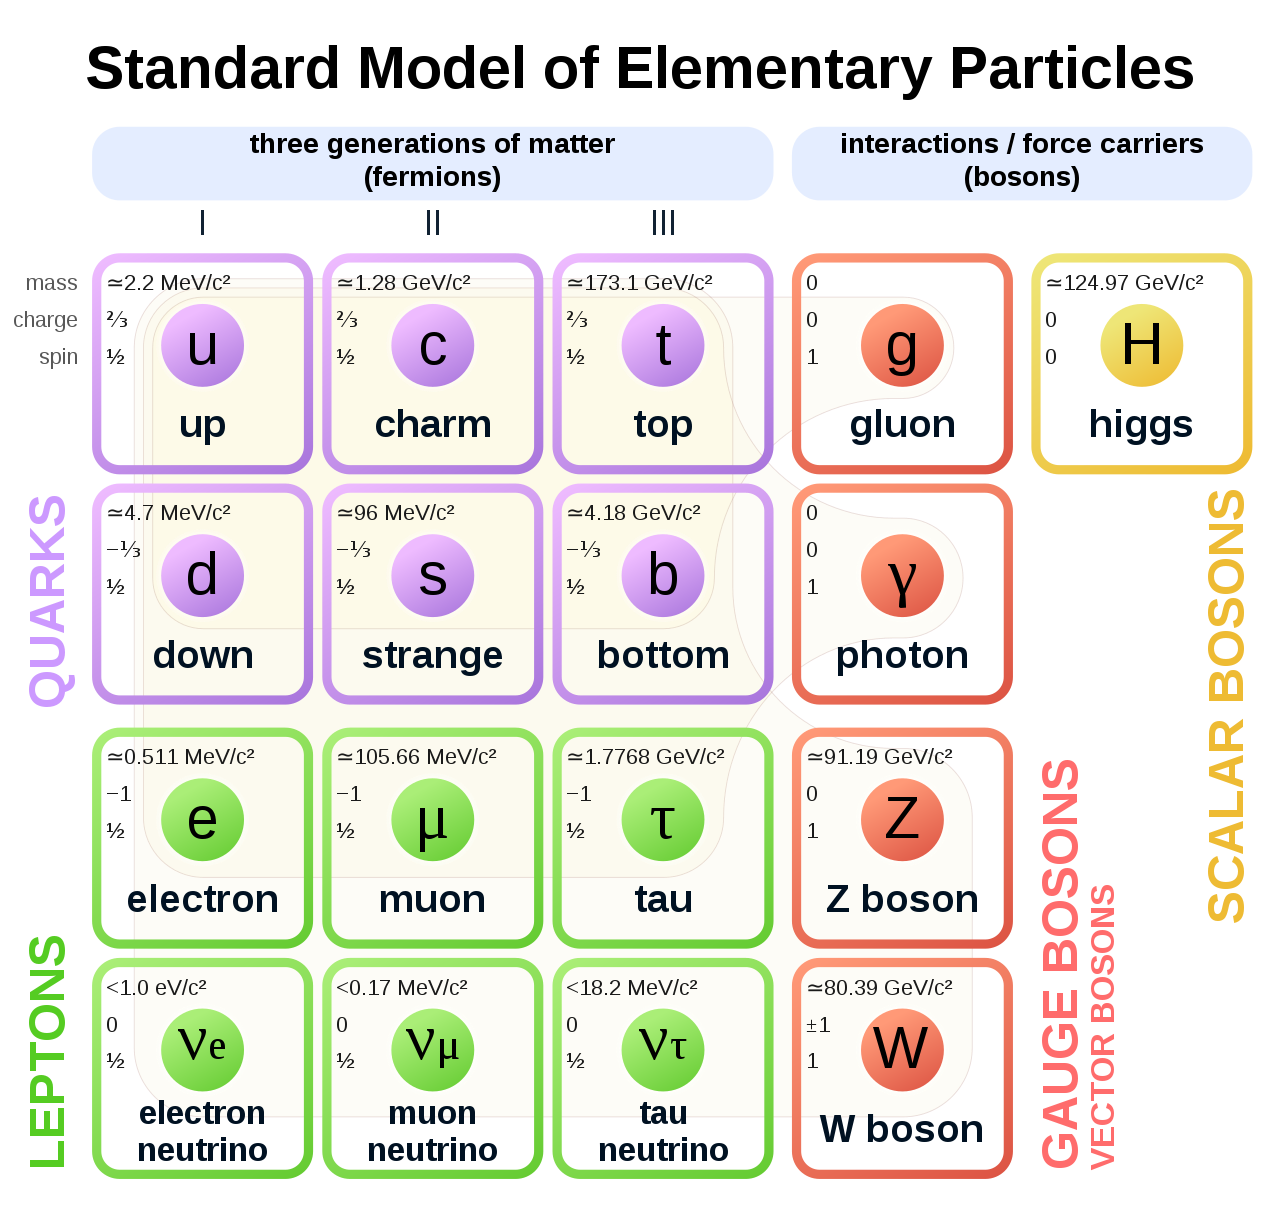
\includegraphics[width=\textwidth,keepaspectratio]{SMwiki.png}
		\caption{The list of particles that enters the \gls{sm}\cite{sm_wiki}. }
		\label{fig::SMwiki}
	\end{figure}
		
An important feature of the \gls{qft} is that particles also interact with physical vacuum. For instance, a charged particle polarizes the physical vacuum, so the vacuum changes the charge of the particle~\cite{Schwinger_polariz}.This interaction with virtual particles depends on the energy scale and so do the observed quantities like charge, mass etc. The \gls{sm} is able to predict parameter evolution, so if the value of a certain input parameter $q_0$ is known at the energy $\Lambda_0$ then it is possible to predict its measurable value $q$ at the energy $\Lambda$. This changing of physical parameters is an integral part of the \gls{qft} and is called \textit{renormalisation} \cite{bogol}, \cite{Glashow:1959wxa}. In the Figure \ref{fig::running} the dependence of the inverted \gls{sm} coupling constants on the energy is shown. 

	 \begin{figure}[htpb]
	 	\centering
	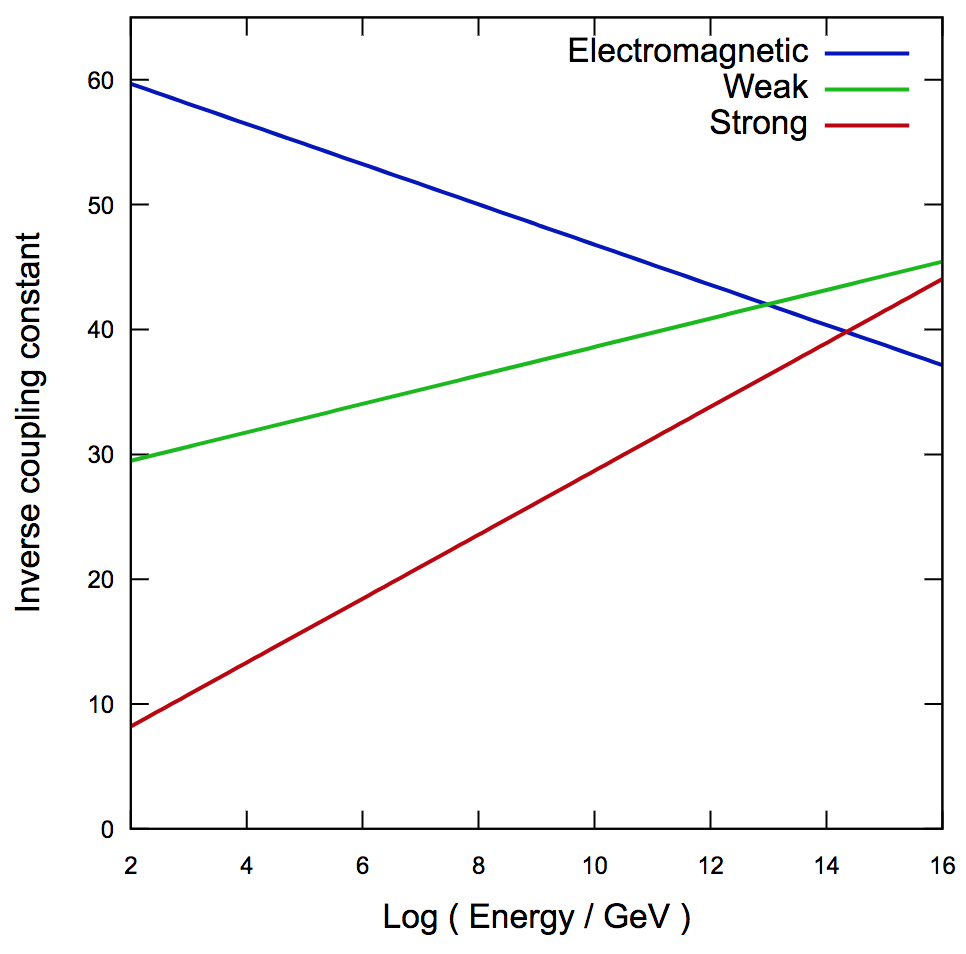
\includegraphics[width=0.6\textwidth,keepaspectratio]{coup_const.png}
	\caption{The running of the inverted \gls{sm} coupling constants \cite{coupl_wiki}. }
	\label{fig::running}
	\end{figure}
As we can see from picture \ref{fig::running} the strong coupling constant is decreasing with the energy. This phenomenon is called \textit{the asymptotic freedom} \cite{Gross,Politzer,Vanyashin}.



\section{Classical fields and gauge invariance principle}
\label{sec::gauge}
A consistent mathematical description of fields appears to be a more challenging task compared to the description of physical objects that have a definite size and shape even in the classical case. The derivation of Maxwell's equations has been a great success and allowed to obtain the first equations of motion of relativistic fields. It has also subseqently led to the understanding of special relativity \cite{einstein,poincare,lorentz}. Although for a more general case of fields other than electromagnetic it would be very useful to adopt a more systematic approach like that of Lagrangian or Hamiltonian in classical mechanics. 

It has turned out that for the relativistic case the Hamiltonian approach was not quite convenient, as the dedicated role of time over other degrees of freedom was in discord with relativistic space-time unification. However it was found possible to describe the fields within the Lagrangian approach. In classic mechanics the action of a mechanical system of $i$ mechanical objects is defined as:
 \begin{equation}
\nonumber
S = \int Ldt = \int \left( \sum_i T_i - U_i \right) dt,
\end{equation}
where $T_i$ and $U_i$ are the kinetic and potential energies of the $i^{th}$ object. Considering that by definition a field exists in every point of space-time, we need to define the Lagrangian density such that $L = \int \mathcal{L}(\phi,\partial_{k}\phi,\dot\phi ) d^3x$, where $\phi$ is a field and $\partial_{k}\phi = \nabla\phi$ - the field gradient, $\partial_{k} = \frac{\partial}{\partial x^{k}}$,  k = 1, 2, 3. Here and further Latin indices run through (1, 2, 3) and are used to denote spatial coordinates, while Greek indices denote space-time coordinates and run though (0, 1, 2, 3). So the action would look like: 
 \begin{equation}
S = \int Ldt =\int \mathcal{L}(\phi,\partial_{\mu}\phi,\dot\phi ) d^4x,
\end{equation}
Now we may use the principle of least action to obtain the equations of motion using the Euler-Lagrange formalism. Let's check it with the example of electromagnetic fields. The Lagrangian density of electromagnetic fields in a vacuum can be written like:
 \begin{equation}
S = -\frac{1}{4}\int F^{\mu \nu}F_{\mu \nu}d^4x.
\end{equation}
The electromagnetic tensor can be defined in terms of electric and magnetic field intensities: $F_{i0}=-F_{0i} = E_i$, $F_{ij} = \epsilon_{ijk}H_k$, where $\epsilon_{ijk}$ is the anti-symmetric Levi-Civita symbol. Alternatively $F_{\mu \nu}$ can be defined in terms of the 4-potential $A_{\mu}$:
 \begin{equation}
F_{\mu \nu} = \partial_{\mu}A_{\nu} - \partial_{\nu}A_{\mu}.
\end{equation}
Now we can safely apply the variational principle, and putting $\delta S=0$ obtain the Maxwell equations in vacuum:
 \begin{equation}
\partial_{\mu}F_{\mu \nu} = 0.
\end{equation}
Noticing the symmetries of the system and using the Noether's theorem\cite{Noether1918} we can find the invariants of electromagnetic field. For example, translational symmetry in time and space ensures conservation of energy and momentum. Let's now consider a symmetry of a different kind. The field potential can be shifted by a gradient of an arbitrary function $\alpha=\alpha(x^\mu)$:

\begin{equation}
\begin{array}{lcl} 
A_{\mu}(x) \rightarrow A^{\prime}_{\mu}(x)  = A_{\mu}(x)+\partial_{\mu}\alpha(x)  \\ 
F_{\mu \nu} \rightarrow F^{\prime}_{\mu \nu}  = \partial_{\mu}(A_{\nu}(x)+\partial_{\nu}\alpha(x))-\partial_{\nu}(A_{\mu}(x)+\partial_{\mu}\alpha(x))=\partial_{\mu}A_{\nu} - \partial_{\nu}A_{\mu}=F_{\mu \nu},
\end{array} 
\end{equation}
where the commutativity of the derivative operator $\partial_{\mu}\partial_{\nu}\alpha(x)=\partial_{\nu}\partial_{\mu}\alpha(x)$ was used.
Let us now consider the electromagnetic theory in the presence of charges and currents:
 \begin{equation}
\mathcal{L} = -\frac{1}{4} F^{\mu \nu}F_{\mu \nu} + j^{\mu}A_{\mu}.
\end{equation}
Now we have an interaction of a field potential $A_{\mu}$ with 4-current $j^{\mu}=(-\rho,j^{i})$. It turns out to be a general property of the field theories: the only form of interaction allowed is between a gauge field and a current.  After applying the gradient field transformation and the least action principle we can obtain the corresponding conservation law:
\begin{equation}
\partial_{\mu}j^{\mu}=0.
\end{equation}
 So this gradient symmetry~\cite{bogol} or as it is called more often gauge symmetry is connected to the conservation of electric current. If a theory is invariant under gauge transformations then it is called a gauge invariant theory. As we have just seen electrodynamics is the simplest example of such a theory. Taking gauge symmetries into consideration \cite{YangMills} has played a huge role in the development of the \gls{sm}.
 
 Gauge degree of freedom can be constrained in arbitrary way by applying additional conditions on the gauge function. This is called fixing the gauge and becomes necessary for the quantization. As a result of a non-trivial procedure it can be show that any physical result must be gauge-invariant, i.e. must not depend on the gauge. 

\section{Quantum electrodynamics}
\label{sec::qed}
\gls{qed} is a theory of interaction between light and electrically charged particles. Historically it was the first quantum field theory to reach good agreement between quantum mechanics and special relativity. \gls{qed} vacuum has zero expectation value.  Nowadays it is considered to be one of the most precise physical theories ever: theory predictions and experiment results agree up to $~O(10^{-11})$. It has also served as a model for the composition of the subsequent parts of the \gls{sm}, describing other fundamental interactions. Let us consider the free Dirac field based Lagrangian:
 \begin{equation}
\mathcal{L} = \bar \psi(x) (i\slashed\partial - m)\psi(x),
\end{equation}
where $\psi$ and $\bar \psi$ are Dirac wave function and its complex conjugate respectively, $\slashed\partial \equiv \gamma_{\mu}\partial^{\mu}$, $\gamma_{\mu}$ is one of the four gamma-matrices and $m$ is the mass of the Dirac field. 
Such a theory, though, would not be physically consistent. This reflects the fact the quantum nature of spin and spinor fields have to be treated as quantum fields. For instance, an attempt to calculate the energy of a Dirac field would lead to a contradiction: the energy would not be positively defined, as some spinors would have negative energies. 

This Lagrangian has an internal symmetry to the U(1) transformation: $\psi\rightarrow e^{-i\alpha(x)}\psi$, \: $\bar\psi\rightarrow e^{i\alpha(x)}\bar\psi$. According to Noether's theorem this symmetry implies current conservation: $j^{\mu}=\bar\psi\gamma^{\mu}\psi$.
Now let's get the combined Lagrangian of electromagnetic and Dirac fields, adding the interaction term:
 \begin{equation}
\mathcal{L} = \mathcal{L}_{Dirac^{free}} + \mathcal{L}_{EM^{free}} + \mathcal{L}_{Interaction} = -\frac{1}{4} F^{\mu \nu}F_{\mu \nu}+\bar \psi(x) (i\slashed\partial -m)\psi(x) - q\bar\psi\gamma^{\mu}A_{\mu}\psi,
\end{equation}
where q represents the elementary electric charge. This Lagrangian above is gauge invariant and can be rewritten in a more convenient form:
 \begin{equation}
\mathcal{L} =  -\frac{1}{4} F^{\mu \nu}F_{\mu \nu}+\bar \psi(x) (i\slashed D -m)\psi(x),
\end{equation}
where $D_{\mu} = \partial_{\mu}-iqA_{\mu}$ is a covariant derivative. If one considers space-time in the presence of a field as curved, then $A_{\mu}$ would play a role of connectivity. It must be noted that values like $m$ and $q$ meaning electron mass and charge\footnote{Charge of the electron is related to the electromagnetic coupling constant.} are the \gls{sm} input parameters mentioned in \ref{sec::sm_gen}.  

Further calculations are to be performed by the means of the quantum field theory formalism that treats interaction terms like a perturbation to the free fields, making power series expansion in the coupling constant. In the case of electrodynamics the coupling constant is quite small so good precision is reached soon. Since the photons do not directly interact with other photons, \gls{qed} allows only one type of vertex - with two electron lines and one photon line. 

\begin{figure}
\label{fig::qed}
\centering
\feynmandiagram [horizontal=a to b, baseline=(current bounding box.center)] {
	i1 -- [fermion] a -- [photon] i2,
	a -- [fermion] b,
	f1 -- [photon] b -- [fermion] f2,
};
\feynmandiagram [horizontal=a to b, layered layout] {
	i1 -- [fermion] a,
	a -- [photon, half left] b,
	a -- [fermion] b,
	b -- [fermion] f1,
};
\feynmandiagram [horizontal=a to b,  layered layout, baseline=(b)] {
	i1 -- [photon] a,
	a -- [fermion, half left] b,
	b -- [fermion, half left] a,
	b -- [photon] f1,
};
\caption{Examples of QED diagrams: Compton scattering, electron self-energy, photon self-energy.}
\end{figure}
Although the tree-level processes and diagrams were well understood by 1930th, the loop diagrams were properly explained only by the end of the 1940th making it possible to obtain numerical results of the higher orders of power series expansion and achieve higher precision predictions for QED processes~\cite{Schwinger_polariz,Schwinger_covar,Feynman_math,Feynman_positrons,Feynman_spacetime,Tomonaga,Dyson_all,Dyson_smatr}. The examples of QED diagrams are presented in figures below.

It must be noted that although immediate photon-photon interaction is impossible, light-by-light scattering is still possible through loops:\\

\begin{center}

\feynmandiagram[layered layout, horizontal=a to b] {
	% Draw the top and bottom lines
	i1 
	-- [photon, edge label = \( \gamma \)] a
	-- [fermion, edge label=\(e \)] b
	-- [photon, edge label=\( \gamma \)] f1 ,
	i2 
	-- [photon, edge label=\( \gamma \)]  c
	-- [anti fermion, edge label=\(e \)]  d
	-- [photon, edge label=\( \gamma \)]  f2,
	%Draw the two internal fermion lines
	{ [same layer] a -- [anti fermion, edge label =\(e\)] c },
	{ [same layer] b -- [fermion, edge label=\(e\)] d},
};\\
\end{center}
This process was theoretically described in 1936~\cite{lbl_th} and experimentally observed 83 years after in heavy ion collisions at the LHC \cite{lbl_exp}.
\section{Electroweak theory and the Higgs mechanism}
All the fermions of the standard model are subject to the weak interaction, so its importance for physical processes can not be underestimated. At low energy the weak interaction manifests itself mainly through flavour-changing decays like beta-decay and muon decay. The electroweak theory was created in the end of 1950s~\cite{Glashow:1959wxa} \cite{weinberg} \cite{Salam1959} thanks to numerous experimental results that allowed to shape its properties. The theory assumed that the electromagnetic and weak fundamental forces are actually manifestation of the same gauge group that has a gauge symmetry $SU(2)_L \cross U(1)$ with massive charged and neutral bosons. A few years later the structure of electroweak vacuum was explained along with the mechanism that has allowed the bosons to gain mass \cite{brout}, \cite{higgs}. Assuming this the Lagrangian of the electroweak theory must consist of three parts~\cite{Hollik_2006}: 
\begin{itemize}
	\item Gauge fields that would mediate the interaction.
	\item Fermions that interact with gauge fields
	\item A scalar Higgs field with non-zero vacuum energy that breaks the $SU(2)_L$ symmetry and couples to the fermions.
\end{itemize}
 \begin{equation}
\mathcal{L}_{EW} = \mathcal{L}_{Gauge} +\mathcal{L}_{Higgs} +\mathcal{L}_{Fermions}
\end{equation}
\subsection{Electroweak gauge fields}
\label{sec::ewk}
As it was already pointed out before, knowing the symmetries of a physical system allows one to compose the gauge fields Lagrangian. The part with U(1) symmetry would look like the electromagnetic field from \ref{sec::gauge} having the hypercharge $Y$, a vector potential $B_{\mu}$ and a gauge coupling $g_1$. The SU(2) field would have 3 vector components $W^{1,2,3}_{\mu}$, three isospin operators $I_1$,$I_2$,$I_3$ and a gauge coupling $g_2$. We can pick the Pauli matrices $\sigma^{i}$ as the representation of generators of the SU(2) group, then the structure constants are $\epsilon_{abc}$ - Levi-Civita symbol.
\begin{equation}
\begin{array}{lcl} 
\mathcal{L_{G}} =  -\frac{1}{4}B_{\mu \nu}B^{\mu \nu} -\frac{1}{4}W^a_{\mu \nu}W^{\mu \nu,a} 
B_{\mu \nu}  =\partial_{\mu}B_{\nu} - \partial_{\nu}B_{\mu}\\ 
W^a_{\mu \nu}  =\partial_{\mu}W_{\nu} - \partial_{\nu}W_{\mu}+g_2\epsilon_{abc}W^b_{\mu}W^c_{\nu},\\ 
\end{array} 
\end{equation}
where the term $g_2\epsilon_{abc}W^b_{\mu}W^c_{\nu}$ appears due to the non-Abelian nature of the SU(2) group (the generators don't commute).


\subsection{Fermion sector}
Each fermion generation expressed as left-handed doublet and right-handed singlets is a fundamental representation of the group $SU(2) \times U(1)$:
\begin{align}
\begin{pmatrix}
\nu_e  \\
e \\
\end{pmatrix}_L,
\begin{pmatrix}
e_R \\
\end{pmatrix},
\begin{pmatrix}
u \\
d \\
\end{pmatrix}_L,
\begin{pmatrix}
u_R \\
\end{pmatrix},
\begin{pmatrix}
d_R \\
\end{pmatrix},
\end{align}

\begin{align}
\begin{pmatrix}
\nu_\mu  \\
\mu \\
\end{pmatrix}_L,
\begin{pmatrix}
\mu_R \\
\end{pmatrix},
\begin{pmatrix}
s \\
c \\
\end{pmatrix}_L,
\begin{pmatrix}
s_R \\
\end{pmatrix},
\begin{pmatrix}
c_R \\
\end{pmatrix},
\end{align}

\begin{align}
\begin{pmatrix}
\nu_\tau  \\
\tau \\
\end{pmatrix}_L,
\begin{pmatrix}
\tau_R \\
\end{pmatrix},
\begin{pmatrix}
b \\
t \\
\end{pmatrix}_L,
\begin{pmatrix}
b_R \\
\end{pmatrix},
\begin{pmatrix}
t_R \\
\end{pmatrix}.
\end{align}

Their quantum states are classified using the following quantum numbers: weak isospin $I_3$, $Q$, weak hypercharge $Y$. Their electric charge can be obtained using the Gell-Mann-Nishijima relation:
  \begin{equation}
Q = I_3+\frac{Y}{2}.
\end{equation}

The fermions are divided by their chirality: only the left-handed particles take part in the charged current of the weak interaction. The left-handed fermion fields of each lepton and quark generation j
  \begin{equation}
    \psi^L_j = \begin{pmatrix}
	\psi^L_{j+}  \\
	\psi^L_{j-}  \\
\end{pmatrix}
  \end{equation}
make SU(2) doublets, with indices $\sigma=\pm$, while the right-handed fermions can be written as singlets:
 \begin{equation}
\psi^R_j = \psi^L_{j\sigma}.  
\end{equation}
Like in the the electromagnetic case we can define the covariant derivative that would ensure the gauge invariance of the Lagrangian:
 \begin{equation}
D_\mu = \partial_{\mu} - ig_2I_aW^a_{\mu}+ig_1\frac{Y}{2}B_{\mu},
\end{equation}
with $I_a \equiv \frac{\sigma_a}{2}$, then fermion Lagrangian takes the following form:
 \begin{equation}
\mathcal{L}_{Fermions} = \sum_f \bar \psi^L_j i \gamma^{\mu}D_{\mu}\psi^L_j +\sum_{f,\sigma} \bar \psi^R_{f,\sigma}  i \gamma^{\mu}D_{\mu}\psi^R_{f,\sigma}  .
\end{equation}

\subsection{Higgs field breaking the symmetry}
\label{sec:symmetry_breaking}
The Higgs field is represented by single complex a scalar doublet field $\Phi(x)$, that has 4 independent components. It spontaneously breaks the  $SU(2)\times U(1)$ gauge symmetry, leaving the $U(1)_{EM}$ symmetry intact. The Higgs field doublet has the hypercharge $Y=1$:
  \begin{equation}
\Phi(x) = \begin{pmatrix}
\phi^{+}(x)  \\
\phi^{0}(x)  \\
\end{pmatrix}.
\end{equation}
The Higgs field Lagrangian with non-zero vacuum expectation value is: 
 \begin{equation}
\mathcal{L}_{Higgs} = (D_{\mu}\Phi)^+(D_{\mu}\Phi)-V(\Phi)+\mathcal{L}_{Yukawa}.
\end{equation}
The gauge invariance of the Higgs Lagrangian is ensured in the traditional way by using the covariant derivative:
 \begin{equation}
D_{\mu} = \partial_{\mu} - ig_2I_aW^a_{\mu}+i\frac{g_1}{2}B_{\mu}.
\end{equation}
The Higgs potential contains the mass term and quartic self-interaction:
 \begin{equation}
V(\Phi) = -\mu^2 \Phi^+\Phi + \frac{\lambda}{4}\partial_{\mu}(\Phi^+\Phi)^2,
\end{equation}
where $\lambda$ stands for the quartic Higgs self-coupling constant and $\mu$ is the mass of the $\Phi$ field. The vacuum expectation value $<\Phi>$ does not vanish:
  \begin{equation}
<\Phi(x)> = \frac{1}{\sqrt(2)}\begin{pmatrix}
0  \\
v \\
\end{pmatrix},\;\;\;\;\; 
v = \frac{2\mu}{\sqrt(\lambda)}.
\end{equation}
Applying the unitarity gauge \cite{weinberg2} we can constrain three out of four degrees of freedom of the Higgs field and rewrite the Higgs doublet in the following way:
  \begin{equation}
 \Phi(x) = \frac{1}{2}\begin{pmatrix}
 	0 \\
 	v+H(x)  \\
 \end{pmatrix},
  \end{equation}
  which leaves us with a physical real neutral scalar field $H(x)$ with 
    \begin{equation}
	M_H=\sqrt{2}\mu.
  \end{equation}
 This real field would couple to itself forming triple and quartic self-coupling vertices, to the gauge fields through the covariant derivatives and to the charged fermions, giving them mass. The Yukawa term in Lagrangian the unitary gauge is:
     \begin{equation}
\mathcal{L}_{Yukawa}=-\sum_f m_f \bar\psi_f\psi_f-\sum_f \frac{m_f}{v} \bar\psi_f\psi_f H,
 \end{equation}
where
\begin{equation}
m_f=g_f\frac{v}{\sqrt{2}}=\sqrt{2}\frac{g_f}{g_2}M_W.
\end{equation}
The Higgs coupling constants to the corresponding fermion flavour are denoted as $g_f$. 
\subsection{Physical interpretation of gauge fields and parameters}
The Higgs coupling to the gauge fields results in the following terms in the Lagrangian:
\begin{equation}
\label{eq::weak_basis}
\frac{1}{2}\frac{g_2^2}{2}v^2(W_1^2+W^2_2)+\frac{v^2}{4}(W^3_{\mu},B_{\mu}) \begin{pmatrix}
g_2^2  & g_1 g_2 \\
g_1 g_2 & g_1^2   \\
\end{pmatrix}
\begin{pmatrix}
W^3_{\mu} \\
B_{\mu}   \\
\end{pmatrix}.
\end{equation}
In order to get the physical meaning of this expression let us make a transition to the basis of physical fields:
\begin{equation}
\begin{array}{lcl} 
W^{\pm}_{\mu}  &=& \frac{1}{\sqrt{2}}(W^{\mp}_{\mu}\mp iW^{\mp}_{\mu})\\ 
\begin{pmatrix} Z_{\mu} \\ A_{\mu}   \\ \end{pmatrix}  &=& \begin{pmatrix} \cos{\theta_{W}} & \sin{\theta_{W}}\\ -\sin{\theta_{W}}& cos{\theta_{W}}   \\ \end{pmatrix} \begin{pmatrix} W^3_{\mu} \\ B_{\mu}   \\ \end{pmatrix},
\end{array} 
\end{equation}
where $\theta_{W}$ is called the weak mixing angle or the Weinberg angle. In the new basis expression \ref{eq::weak_basis} has transparent physical sense:
\begin{equation}
M^2_W W^+_{\mu}W^{-\mu} +\frac{1}{2} (A_{\mu},Z_{\mu})\begin{pmatrix}
0 & 0 \\
0 & M^2_Z   \\
\end{pmatrix}
\begin{pmatrix}
A_{\mu} \\
Z_{\mu}   \\
\end{pmatrix},
\end{equation}
with
\begin{equation}
\begin{array}{lll} 
M_W &= & \frac{1}{2} g_2 v\\ 
M_Z &=& \frac{1}{2} \sqrt{g_1^2+g_2^2} v.
\end{array} 
\end{equation}
The mixing angle $\theta_W$ also has a very clear physical meaning:
\begin{equation}
\cos{\theta_W}=\frac{g_2}{g_1^2+g_2^2}=\frac{M_W}{M_Z}.
\end{equation}
With $A_{\mu}$ having a sense of electromagnetic potential its coupling to the electron must have a physical meaning of the electric charge $e=\sqrt{4\pi\alpha}$ we can express $e$ in terms of gauge couplings:
\begin{equation}
e=\frac{g_1 g_2}{g_1^2+g_2^2}, \;\;\;\;g_2=\frac{e}{\sin{\theta_W}},\;g_1=\frac{e}{\cos{\theta_W}} .
\end{equation}
Thus the demonstrated Weinberg rotation (see Fig. \ref{fig::weiberg_rotation}) replaces the original parameters $g_1$, $g_2$, $\lambda$, $\mu^2$, $g_f$ by another set of measurable values $e$, $M_W$, $M_Z$, $M_H$, $m_f$ which are the input parameters of the \gls{sm}.


\begin{figure}[htpb]
	\centering
	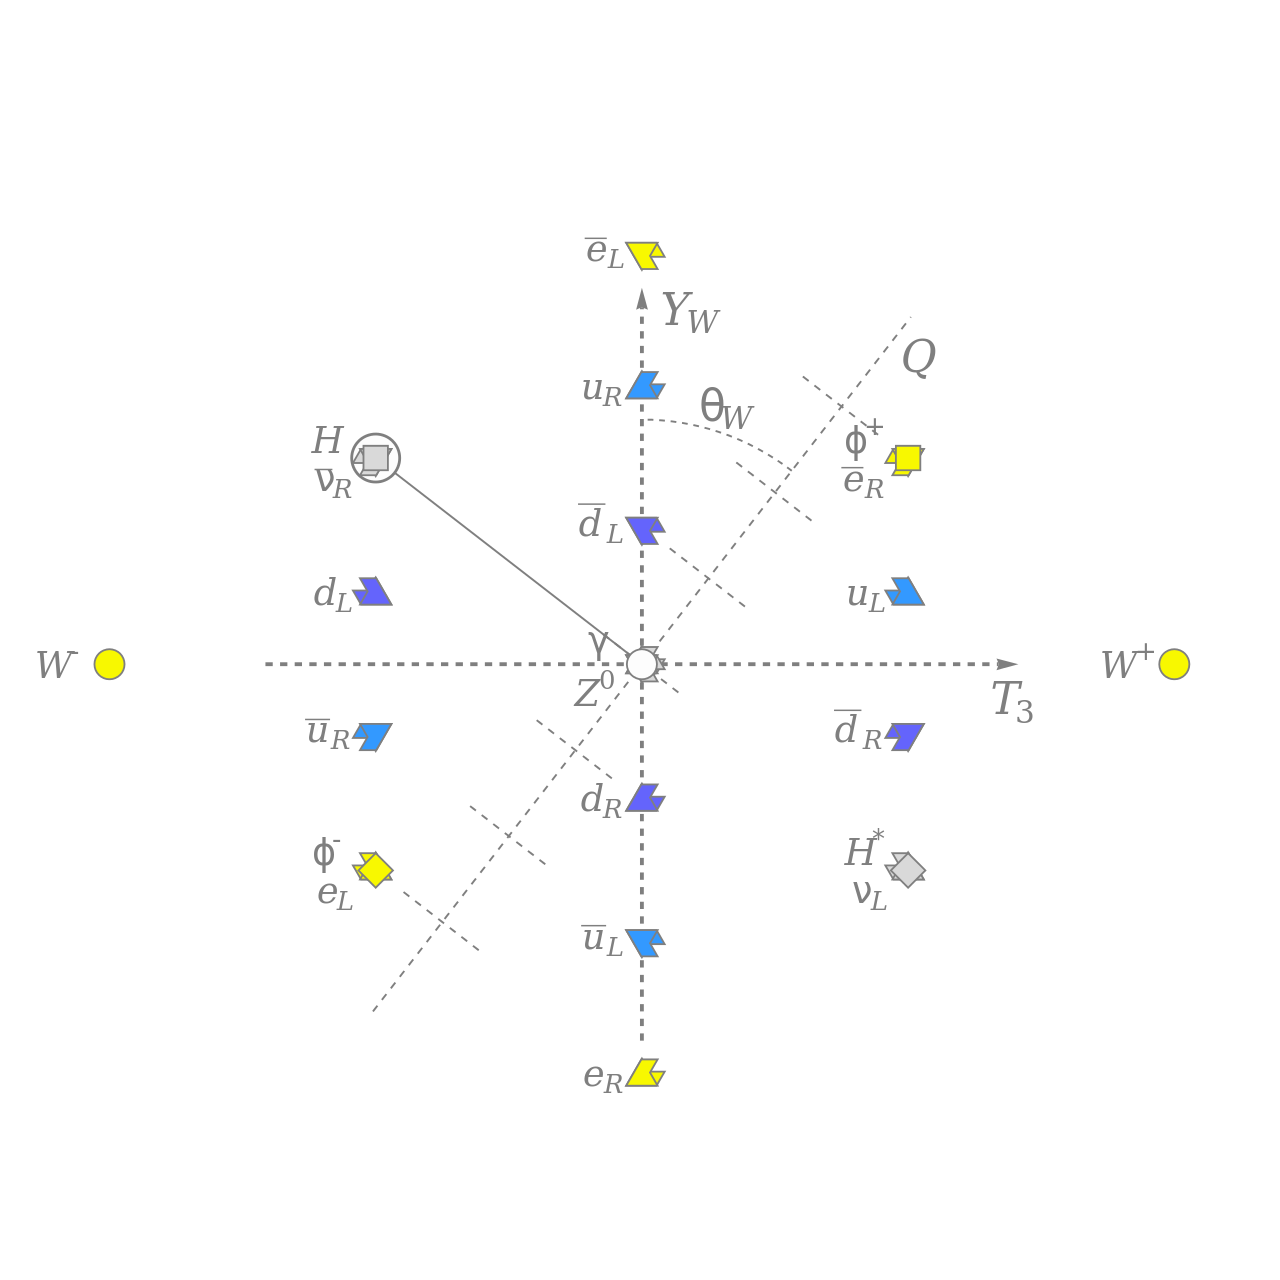
\includegraphics[width=0.65\textwidth,keepaspectratio]{weinb.png}
	\caption{Electroweak sector and the Weinberg rotation \cite{coupl_wiki}. }
	\label{fig::weiberg_rotation}
\end{figure}

\section{Chromodynamics}
\gls{qcd} is a non-Abelian gauge theory that describes strong interaction. \gls{qcd} is symmetric under unbroken SU(3) colour symmetry, so the interaction scheme is built in the same way as electromagnetic and electroweak theories. To preserve the gauge invariance the gauge field of gluons is introduced with 8 components, since SU(N) group has $N^2-1$ independent elements. The gluons are massless vector bosons like the photons, although because of the non-Abelian nature of the gauge group they couple not only to the fermions but also to the other gluons. The gauge invariant QCD Lagrangian with kinetic term containing covariant derivative would look like:
\begin{equation}
\begin{array}{lll} 
	\mathcal{L}_{QCD} &=& -\frac{1}{4}F^a_{\mu\nu}F_a^{\mu\nu} + \bar\psi_a(i(\gamma^{\mu}D_{\mu})^{ab} - m\delta^{ab})\psi_b,\\
	F^a_{\mu\nu}  &=& \partial_{\mu}A_{\nu}^a-\partial_{\nu}A^a_{\mu}+g_sf^{abc}A^b_{\mu}A^c_{\nu},\\
	D_{\mu} &=& \partial_{\mu} + ig_s A_{\mu}^at_a.
\end{array} 
\end{equation}
with $\psi$ being the quark field, m is the mass of the quark, a,b = 1, 2, ..., 8 are the colour indices, $g_s$ is the strong coupling constant, $f^{abc}$ are the structure constants of the SU(3) group and $t_a$ are the generators of the SU(3) group. \\
As it was already mentioned in \ref{sec::qed} quantitative calculations in \gls{qft} treat particle interaction as a perturbation to the free field theory. The coupling constant is considered to be a small parameter so every next power of the coupling constant is much smaller than the previous one. Due to asymptotic freedom the constant $\alpha_s$ becomes small at higher energies and allows perturbative calculations. But at a certain energy scale called $\Lambda_{QCD}\approx200$ MeV, \gls{qcd} becomes non-perturbative. It means we may no longer assume that interaction is a small perturbation of the free fields. This phenomenon causes the \textit{colour confinement}.

	 \begin{figure}[htpb]
	 	\centering
	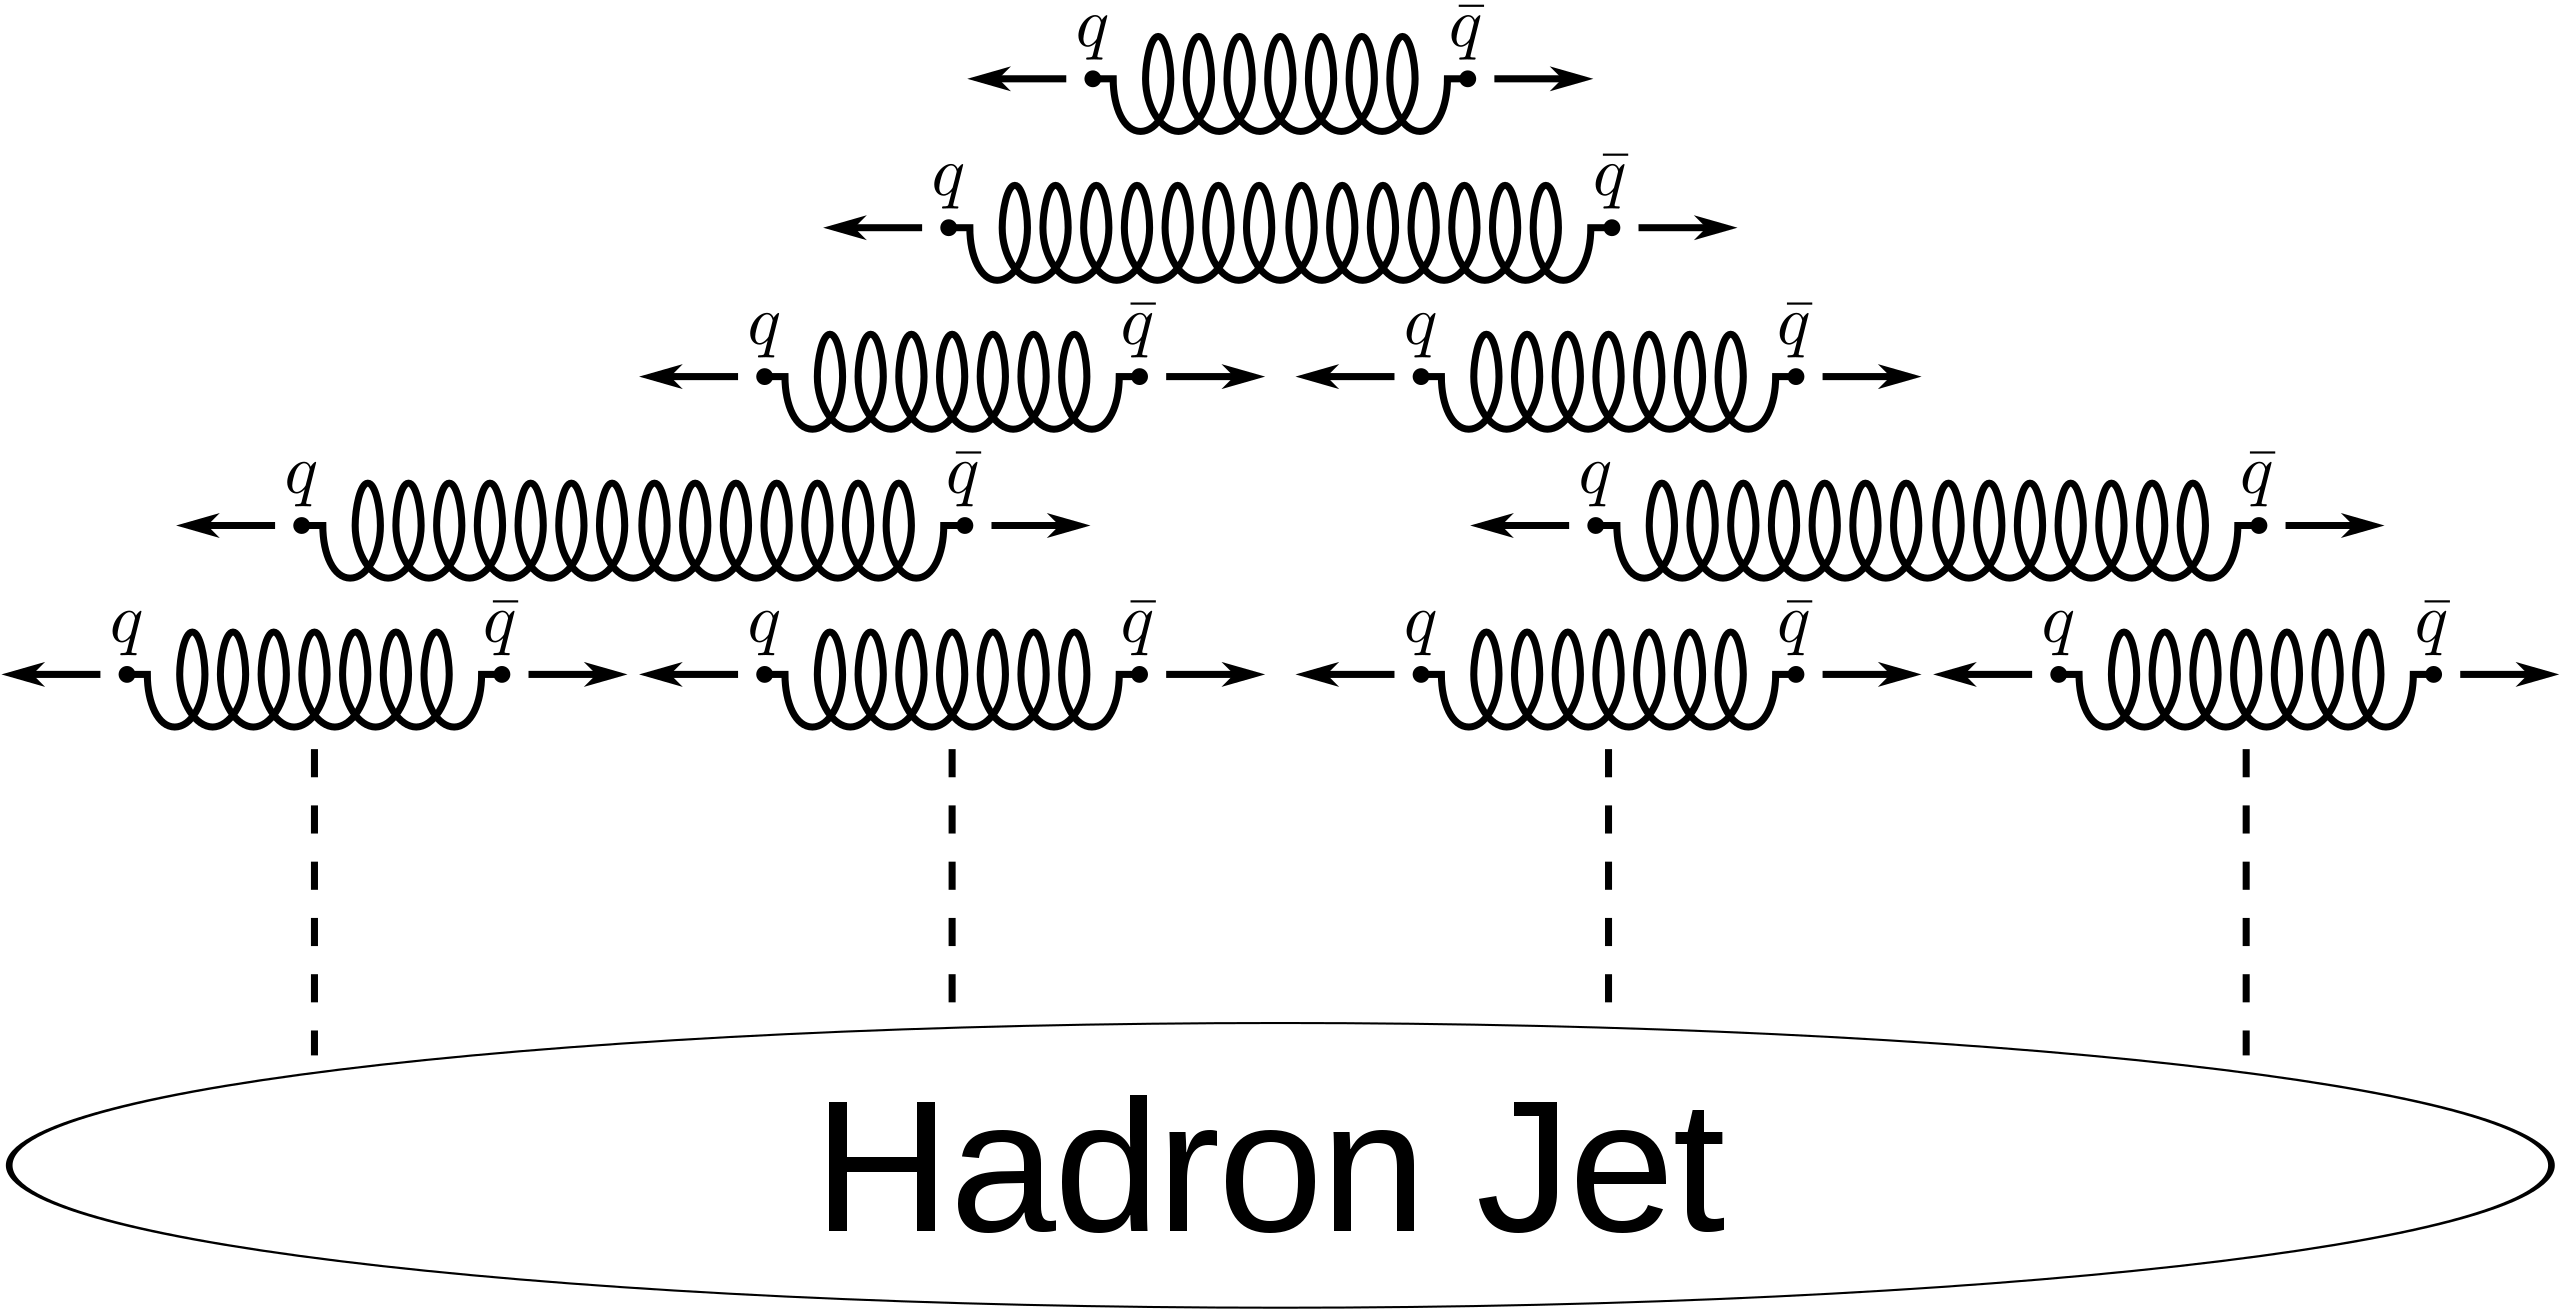
\includegraphics[width=0.75\textwidth,keepaspectratio]{confinement.png}
	\caption{The formation of a hadron jet \cite{conf_wiki}. }
	\label{fig::jet}
	\end{figure}
Because of colour confinement we can only observe colourless objects like baryons and mesons, but not quarks and gluons. If a high-energetic parton gets torn out of a hadron then it creates an avalanche-like process creating quark-antiquark pairs until it fully hadronizes (see Fig. \ref{fig::jet}) neutralizing its colour. Such an avalanche is called a hadronic jet. 

Currently there is no viable physical theory that would describe \gls{qcd} vacuum and low-energy behaviour of quarks and gluons. This also means that although nuclear forces are evidently residuals of the QCD interaction of partons within the baryons, there is no continuity between \gls{qcd} and nuclear physics. Confinement and low-energy \gls{qcd} remain an unsolved problem of modern physics. 



\newpage
\chapter{The Large Hadron Collider}
    \chapterprecishere{
        ``Potentielle citation sans aucun rapport avec le sujet"\par\raggedleft--- \textup{Personne inconnue}, contexte à déterminer
    }
    
   
        
    \section{Introduction}
    
        The study of elementary particles naturally demands a stable source of particles. At the dawn of particle physics the two main sources were radioactive materials and the cosmic rays. However soon researchers became in need of a more reliable source of particles in terms of particle energy, luminosity and experimental repeatability. This has commenced the era of particle accelerators.\\
        The first examples of particle accelerators were designed in late 1920s and early 1930s. Two different designs emerged: linear and circular. The former accelerates particles via electric field during the single pass through the machine, while the latter uses magnetic field to make accelerated particles go in circles allowing to re-accelerate the same beam many times. On the other hand the circular design comprises energy losses due to Bremsstrahlung radiation.\\
        In the second half of the XX century the accelerators gradually got bigger and bigger in both size and center-of-mass energy of the accelerated particles. This has allowed to create an experimental basis for the development of modern particle physics, notably the Standard Model.\\
        Up to this day the biggest particle accelerator with the highest center-of-mass energy is the Large Hadron Collider (LHC). LHC is a circular collider that lies in a tunnel of 27 km under the French-Swiss border next to Geneva \cite{Bruening}. In 2012 two biggest experiments of LHC have claimed the discovery of the Higgs boson, the last elementary particle predicted by the Standard Model which was not yet discovered by that time. \cite{higgs_atlas}, \cite{higgs_cms}.
        
        \section{The principle of a circular collider}
        
        Circular colliders - how they work and why they are circular. Cyclotron frequency.
Pipes, dipoles, quadrupoles, RF cavities, interaction points.

        \section{The LHC acceleration sequence}
        A few sentences and pictures about the chain between a ballon of hydrogen and the collisions at the IPs. 

        \section{Bunching and luminosity }
How and why the beam is bunched. How the luminosity is delivered to the IP and why it is a very important observable

        \section{LHC performance during the low-mu run}
A few plots and tables containing info about the delivered and collected luminosity

%\newpage
%\chapter{The Large Hadron Collider}
   The chapter on the Large Hadron Collider provides a bit of overview on the purpose and operation principle of the collider. It also provides the information on the special low pile-up run which is the main source of experimental data for the W boson transverse momentum measurement analysis.
   
   
    \section{Introduction} 
        The study of elementary particles naturally demands a stable source of particles. At the dawn of particle physics the two main sources were radioactive materials and cosmic rays. However soon researchers became in need of a more reliable source of particles in terms of particle energy, luminosity and experimental repeatability. This has commenced the era of particle accelerators.\\
        The first examples of particle accelerators were designed in the late 1920s and in the early 1930s. Two different designs emerged: linear and circular. The former accelerates particles via electric field during the single pass through the machine, while the latter uses magnetic field to make accelerated particles go in circles allowing to re-accelerate the same beam many times. On the other hand the circular design comprises energy losses due to Bremsstrahlung radiation.\\
        In the second half of the XX$^{th}$ century the accelerators gradually got bigger and bigger in both size and centre-of-mass energy of the accelerated particles. This has allowed to create an experimental basis for the development of modern particle physics, notably the Standard Model.\\
        Up to this day the biggest particle accelerator with the highest centre-of-mass energy is the Large Hadron Collider (LHC). The LHC is a circular collider that lies in a tunnel of 27 km under the French-Swiss border next to Geneva \cite{Bruning:2668521}. In 2012 the two biggest experiments of LHC have claimed the discovery of the Higgs boson, the last elementary particle predicted by the Standard Model which was not yet discovered by that time. \cite{higgs_atlas}, \cite{higgs_cms}.
        
        \section{The LHC running sequence}
                   \begin{figure}[htpb]
        	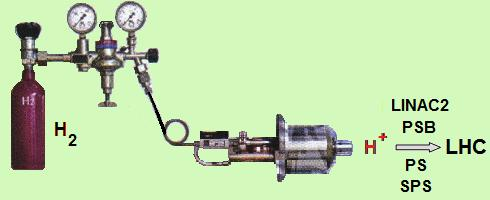
\includegraphics[width=\textwidth,keepaspectratio]{hydro_tank.jpg}
        	\caption{A hydrogen tank supplies LHC with protons \cite{hydro}.}
        	\label{fig::hydro}
        \end{figure}
        	
        It takes quite a journey for a proton to travel from a hydrogen tank (Fig. \ref{fig::hydro}) into one of the LHC's collision points. A resourceful system of pre-accelerators is necessary to make the proton beam ready to get injected into one of the two LHC beam pipes. The LHC accelerator complex was not built from scratch - it uses vast CERN infrastructure, that was built for the previous particle physics experiments. \\
        After stripping the electrons off the atoms of hydrogen using a magnetic field the yielded protons get accelerated to the energy of 50 MeV by the Linac 2\footnote{After Run 2 the Linac 2 has been decommissioned to be succeeded by Linac 4.} \cite{sequence}. After that the beam gets into the Proton Synchrotron Booster (PSB) to be accelerated to 1.4 GeV. The next link of the pre-acceleration chain is the Proton Synchrotron (PS) - a true veteran among CERN accelerators that first accelerated protons in 1959 breaking the world record in acceleration energy. Currently thanks to PSB and other modifications it can sustain proton beam intensity ~1000 times larger than back in 1959. The PS accelerates the beam up to 25 GeV and conveys it further to the Super Proton Synchrotron (SPS) - the second-largest particle accelerator at CERN. Back in 1983 the massive electroweak bosons were discovered at the SPS but even now it serves as a main accelerator for the NA61/SHINE, NA62 and COMPASS experiments. The SPS raises the beam energy to 450 GeV and finally injects it into the LHC beam pipes (see Fig \ref{fig::layout}).\\
   

	\begin{figure}[htbp]
	\begin{subfigure}[t]{0.48\textwidth}
		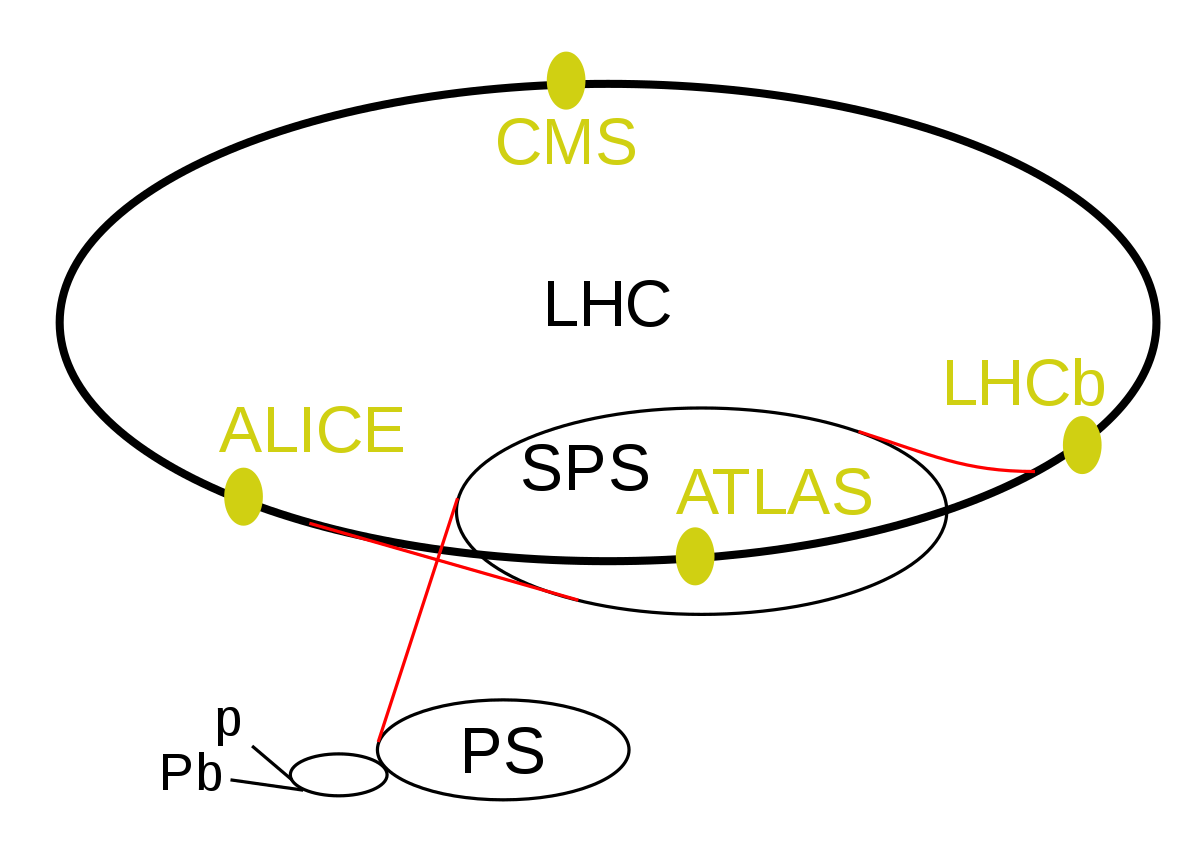
\includegraphics[width=\textwidth,keepaspectratio]{LHC.png}
		\caption[Acceleration sequence]{Acceleration sequence \cite{sequence}.}
		\label{fig::seq}
	\end{subfigure}
	\hfill
	\begin{subfigure}[t]{0.48\textwidth}
		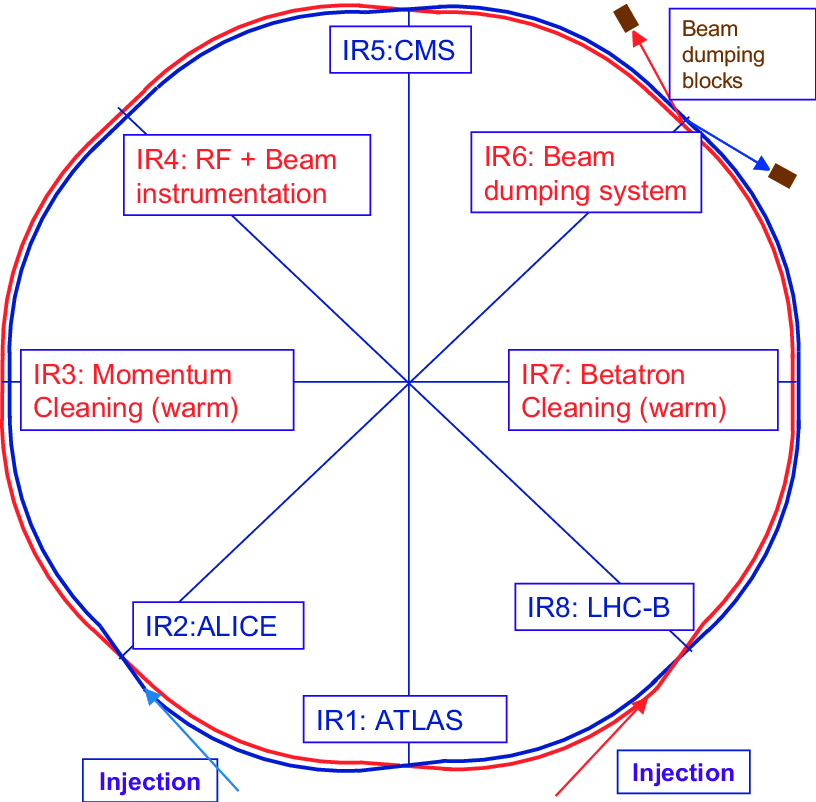
\includegraphics[width=\textwidth,keepaspectratio]{Layout.png}
		\caption[Beam pipes]{LHC beam pipes and crossing points.}
		\label{fig::pipes}
	\end{subfigure}
	\caption{Schematic depiction of the LHC ring.}
	\label{fig::layout}
\end{figure}

     The LHC has inherited its 27 km tunnel from the predecessor, an electron-positron collider called Large Electron-Positron (LEP). However, all the LEP hardware has been replaced to sustain the conditions of the LHC beam. About 2/3 of the LHC circumference length is occupied by the dipole magnets that bend the trajectory of the proton beam to keep it within the pipe. These magnets use superconducting coils that conduct a current of 11080 amperes to produce a magnetic field of 8.3 Tl.\\
     Proton acceleration is maintained by the radio-frequency (RF) cavities (Fig. \ref{fig::rf_cavities}). Besides the acceleration particles the RF cavities are also responsible for beam bunching i.e. separating the beam into a train of separated particle packs, each containing about $10^{11}$ protons. During LHC Run 2 the bunches were separated by 7 meters (25 ns) with a maximum of 2556 circulating bunches.
	\begin{figure}[htbp]
	\begin{subfigure}[t]{0.48\textwidth}
		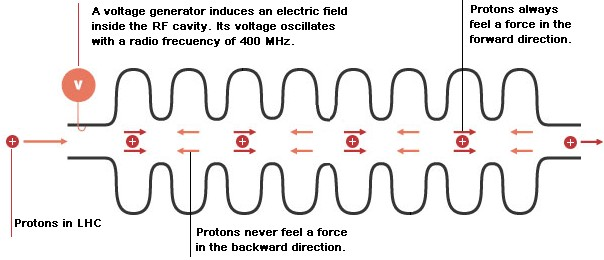
\includegraphics[width=\textwidth,keepaspectratio]{rf_cavities.jpg}
		\caption[RF Cavities]{The RF cavities \cite{rf_cavities}.}
		\label{fig::rf_cavities}
	\end{subfigure}
	\hfill
	\begin{subfigure}[t]{0.48\textwidth}
		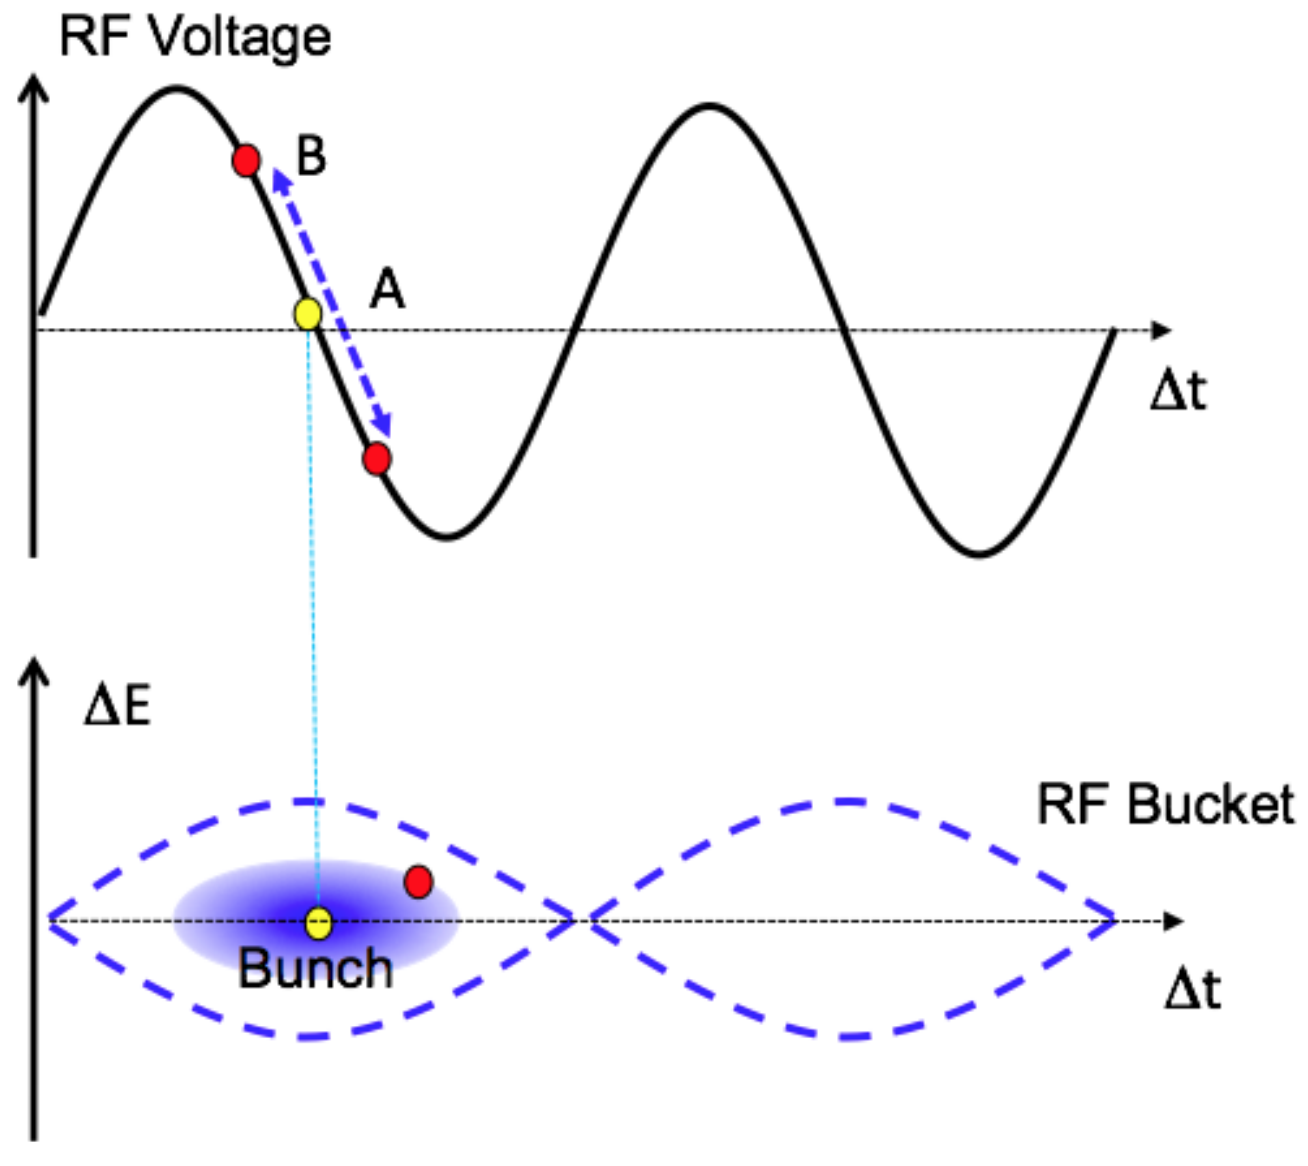
\includegraphics[width=\textwidth,keepaspectratio]{bunch0.png}
		\caption[Beam pipes]{Bunch behaviour at the RF cavities \cite{Wilson:513326}.}
		\label{fig::bunching}
	\end{subfigure}
	\caption{Bunching at RF cavities}
	\label{fig::bunch_at_rf}
\end{figure}
	The LHC has four crossing points, where the two beams are crossed in order to collide protons. Naturally, the particle detectors are installed at these four points. Before getting directed at the crossing point the beams get squeezed to make their cross-section as small as 16 $\mu m^2$ (Fig \ref{fig::2beams}).  	

	\begin{figure}[htbp]
	\begin{subfigure}[t]{0.48\textwidth}
		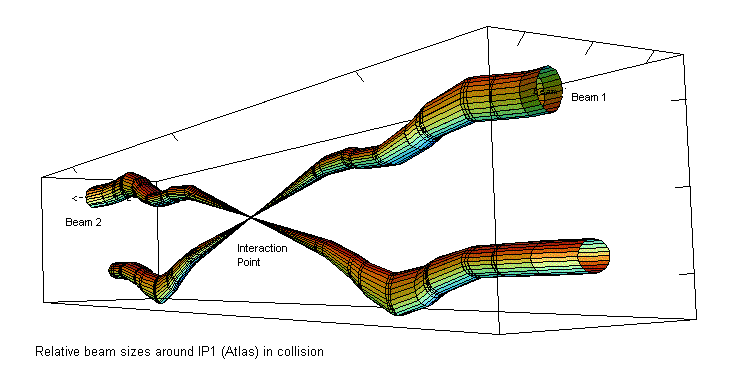
\includegraphics[width=\textwidth,keepaspectratio]{2-beams-IP.png}
		\caption[Two beams]{The two beams getting squeezed at the IP \cite{2beams}.}
		\label{fig::2beams}
	\end{subfigure}
	\hfill
	\begin{subfigure}[t]{0.48\textwidth}
		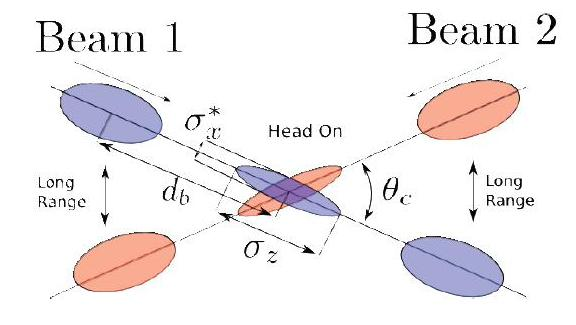
\includegraphics[width=\textwidth,keepaspectratio]{bunch_crossing.jpg}
		\caption[Bunches colliding]{Bunches at the collision point \cite{collisions}.}
		\label{fig::bunches_collision}
	\end{subfigure}
	\caption{Bunch crossing at the LHC.}
	\label{fig::interaction_point}
	\end{figure}
	In order to estimate the number of single proton-proton interactions in the crossing beams a value called instantaneous luminosity (simply called luminosity) is introduced. It is the proportionality factor between the number of events per second $dR/dt$ and the cross-section $\sigma_p$:
	 \begin{equation}
	\nonumber
	\frac{dR}{dt} = \mathcal{L} \cdot \sigma_p.
	\end{equation}
	For the case of head-on collisions the luminosity would equal to \cite{Lumi}:
	\begin{equation}
	\mathcal{L} = \frac{N_1N_2fN_b}{4\Pi \sigma_x \sigma_y},
	\end{equation}
	with $N_1$ and $N_2$ being the intensities of the two colliding beams, $f$ is the revolution frequency, $N_b$ - the number of bunches per beam, $ \sigma_x,\sigma_y$ - the r.m.s. beam widths in the corresponding dimensions, assuming that the bunches in both beams have the same size and Gaussian profiles. \\

	Head-on crossing of the beams would ensure maximal luminosity given the same beams, but on the other hand the measurement would suffer from unwanted beam-to-beam effects. To avoid it the beams at the LHC are crossed at an angle, which is called the crossing angle (see Fig. \ref{fig::bunches_collision}). 
	For the case of head-on collisions the luminosity gets a factor $\mathcal{F} $ \cite{Lumi}:
	\begin{equation}
	\mathcal{L} = \frac{N_1N_2fN_b}{4\Pi \sigma_x \sigma_y} \cdot \mathcal{F},\\
	\end{equation}
	with geometric factor
	\begin{equation}
	\nonumber
	\mathcal{F} = \frac{1}{\sqrt{ 1+\left(  \frac{\sigma_s}{\sigma_x}  \frac{\theta_c}{2} \right) }},
	\end{equation}
	where $\sigma_s$ is the r.m.s. of the bunch length and $\theta_c$ is the crossing angle. Varying the parameters like beam intensity, bunch spacing, beam profile, crossing angle and others becomes a flexible tool for luminosity control. This comes in handy for different physics analysis, as some processes are rare and demand as much luminosity as possible (this is true, for example, for most of the Higgs studies), whereas the others suffer from high pile-up conditions.
	The instantaneous luminosity integrated over a period of time is called the integrated luminosity:
	\begin{equation}
	\mathcal{L}_{int} = \int_0^{T} \mathcal{L}(t) dt,
	\end{equation}
	and is directly related to the number of observed events $\mathcal{L}_{int} \cdot \sigma_p = N_{events}$. A precise measurement of the integrated luminosity is crucial for the LHC results since the uncertainty on it impacts most of the analyses. A comprehensive overview on the luminosity determination at proton colliders can be found here \cite{lumi_witold}. Absolute luminosity measurements at the LHC are performed predominantly using the van-der-Meer (vdM) scan method \cite{vdm1}, \cite{vdm2}. 
	
        \section{Special low pile-up run during LHC Run 2}
        During the Run 2 that lasted from 2015 to 2018 the ATLAS experiment has collected 146.9 $fb^{-1}$ of data under different bunch crossing conditions (see Fig. \ref{fig::run2lumi}). However, the precise measurement of the W boson-related processes demands special conditions. High number of proton-proton collisions per bunch crossing leads to contamination of the final state signal with soft collisions products. This effect, known as pile-up, complicates object reconstruction and results in systematic uncertainties growth. For this reason two special runs with low number of interactions per bunch crossing have been performed by the LHC in 2017 and 2018 at the energies of 5 and 13 TeV. Table \ref{tab:lowmu} contains information on the data collected at ATLAS experiment during the special low pile-up run with $<\mu> \approx 2$.\\
		 \begin{figure}[htpb]
			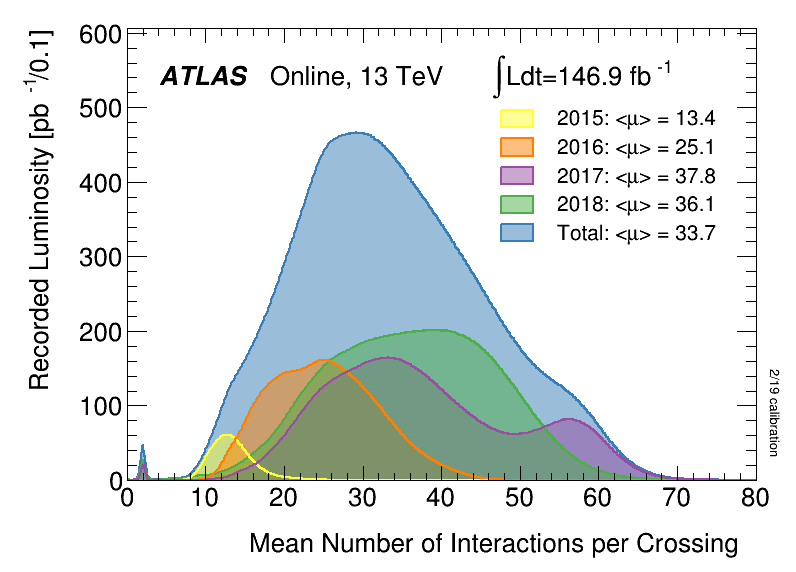
\includegraphics[width=\textwidth,keepaspectratio]{mu_2015_2018.png}
			\caption{ Number of Interactions per bunch crossing in \gls{atlas} Run 2 \cite{run2lumi}. The little bump around $\mu \approx 2$ corresponds to special low pile-up runs.}
			\label{fig::run2lumi}
			\end{figure}
			\begin{table}
			\centering			
			\begin{tabular}{|l|c|c|c|}
			\hline
			\textbf{Collision energy} & \textbf{Year}& \textbf{Integrated luminosity, $pb^{-1}$ }&  Total uncertainty, \%\\
			\hline
			5 TeV  & 2017 & 258& 1.6\\
			13 TeV  & 2017 & 148& 2.1 \\
			13 TeV  & 2018 & 193& 1.5\\
			\hline
			\end{tabular}
			\caption{Energy and luminosity of the special low-mu runs.}
			\label{tab:lowmu}
			\end{table}
%\newpage
%\chapter{Electromagnetic shower shapes correction in the electromagnetic calorimeter }
    \chapterprecishere{
        ``Potentielle citation sans aucun rapport avec le sujet"\par\raggedleft--- \textup{Personne inconnue}, contexte à déterminer
    }

  \section{Introduction}
  The design and functionality of the ATLAS electromagnetic calorimeter was described in \ref{emc}. Let's consider a bit more in detail the physical processes happening in the \gls{emc}. \\
  It order to measure particle's energy within the calorimeter we must make the particle to loose its entire energy within the calorimeter. For the electrons and photons with energies over few MeV (which is the case for the ATLAS experiment) the primary energy loss mechanism lies in bremsstrahlung radiation and pair creation). The two processes complete each other, so when a high-energy electron or photon gets into the calorimeter, it creates an avalanche-like processus called the electromagnetic shower when a bremsstrahlung-radiated photons create more electron-positron pairs which in turn radiate more bremsstrahlung photons and so on and so forth (see fig. \ref{fig::em_shower}.)\\
  	\begin{figure}[htbp]
  	\begin{subfigure}[t]{0.5\textwidth}
  		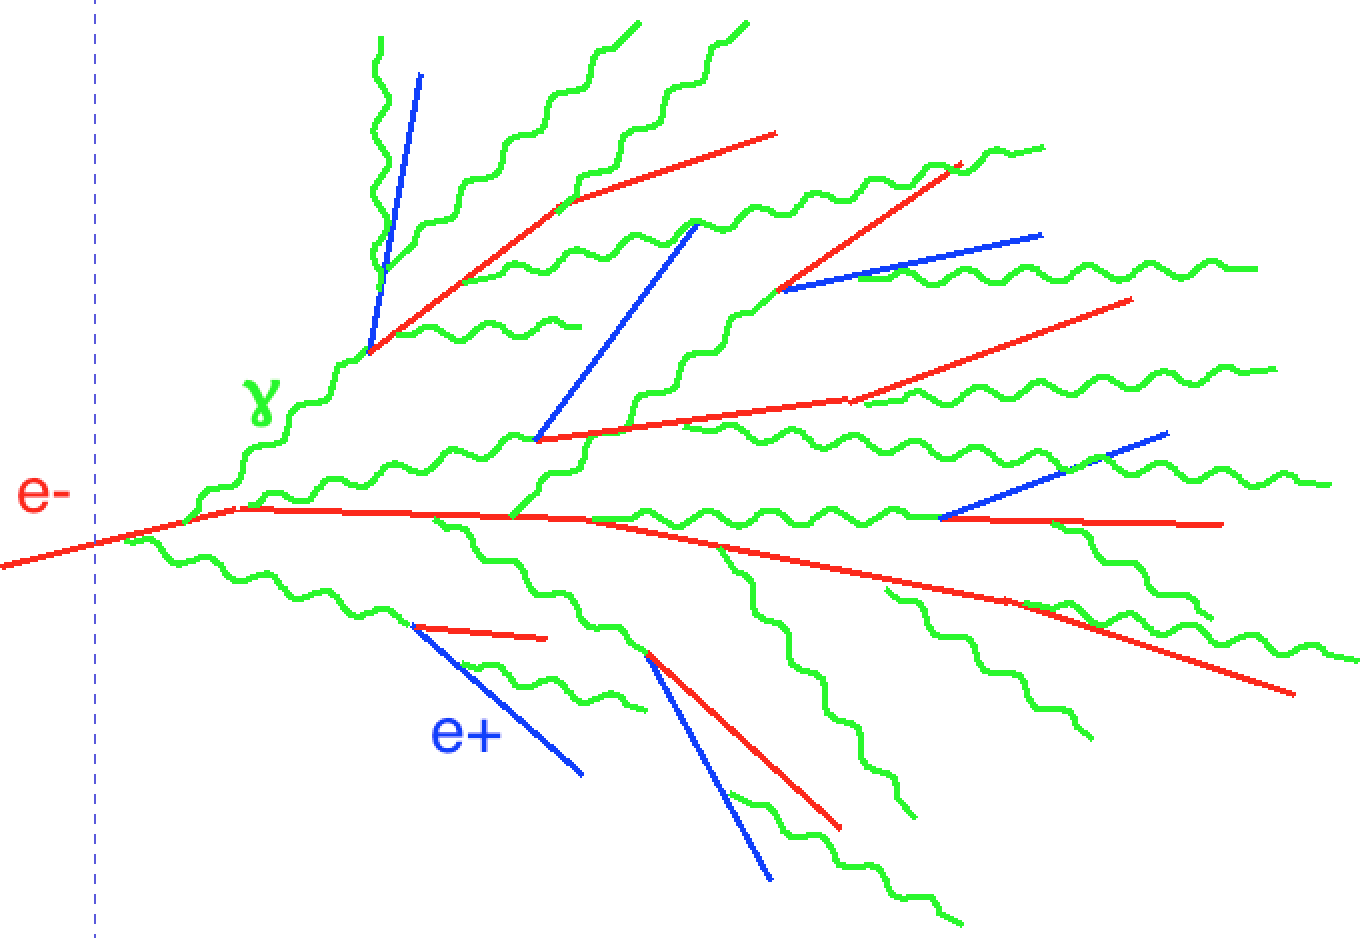
\includegraphics[width=\textwidth,keepaspectratio]{em_shower.png}
  		\caption[Started by an electron]{Initiated by an electron}
  		\label{fig::id}
  	\end{subfigure}
  	\hfill
  	\begin{subfigure}[t]{0.5\textwidth} 
  		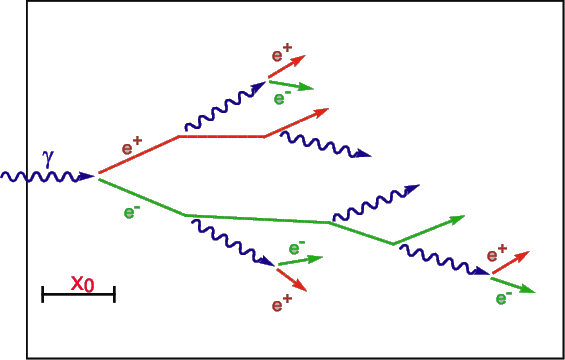
\includegraphics[width=\textwidth,keepaspectratio]{emshower.png}
  		\caption[Started by a $\gamma$-photon]{Initiated by a $\gamma$-photon}
  		\label{fig::pd}
  	\end{subfigure}
  	\caption{The schematic portrayal of EM shower development}
  	\label{fig::em_shower}
  \end{figure}
    The longitudinal and transverse development of the shower depends on the type of the initial particle and on its energy. The energy is well measured by the calorimeter, but identifying the particle still remains a challenging task. The transverse granularity of the ATLAS calorimeter allows to resolve the energy distribution withn the electromagnetic shower in the transverse plane. This information can later be used for particle identification.\\
  When an e/$\gamma$ particle hits the calorimeter its footprint in the second layer of the calorimeter is visible as a cluster of calorimeter cells centered at the central cell having the most energy deposited (sometimes referred to as "the hottest cell"). Roughly 90$\%$ of shower energy is contained in the core 3x3 cells.  We have considered a cluster of 7x11 ($\eta$ x $\phi$) cells, which is schematically depicted on fig. \ref{fig::profile_log}.
  
  
    	\begin{figure}[htbp]
  	\begin{subfigure}[t]{0.5\textwidth}
  		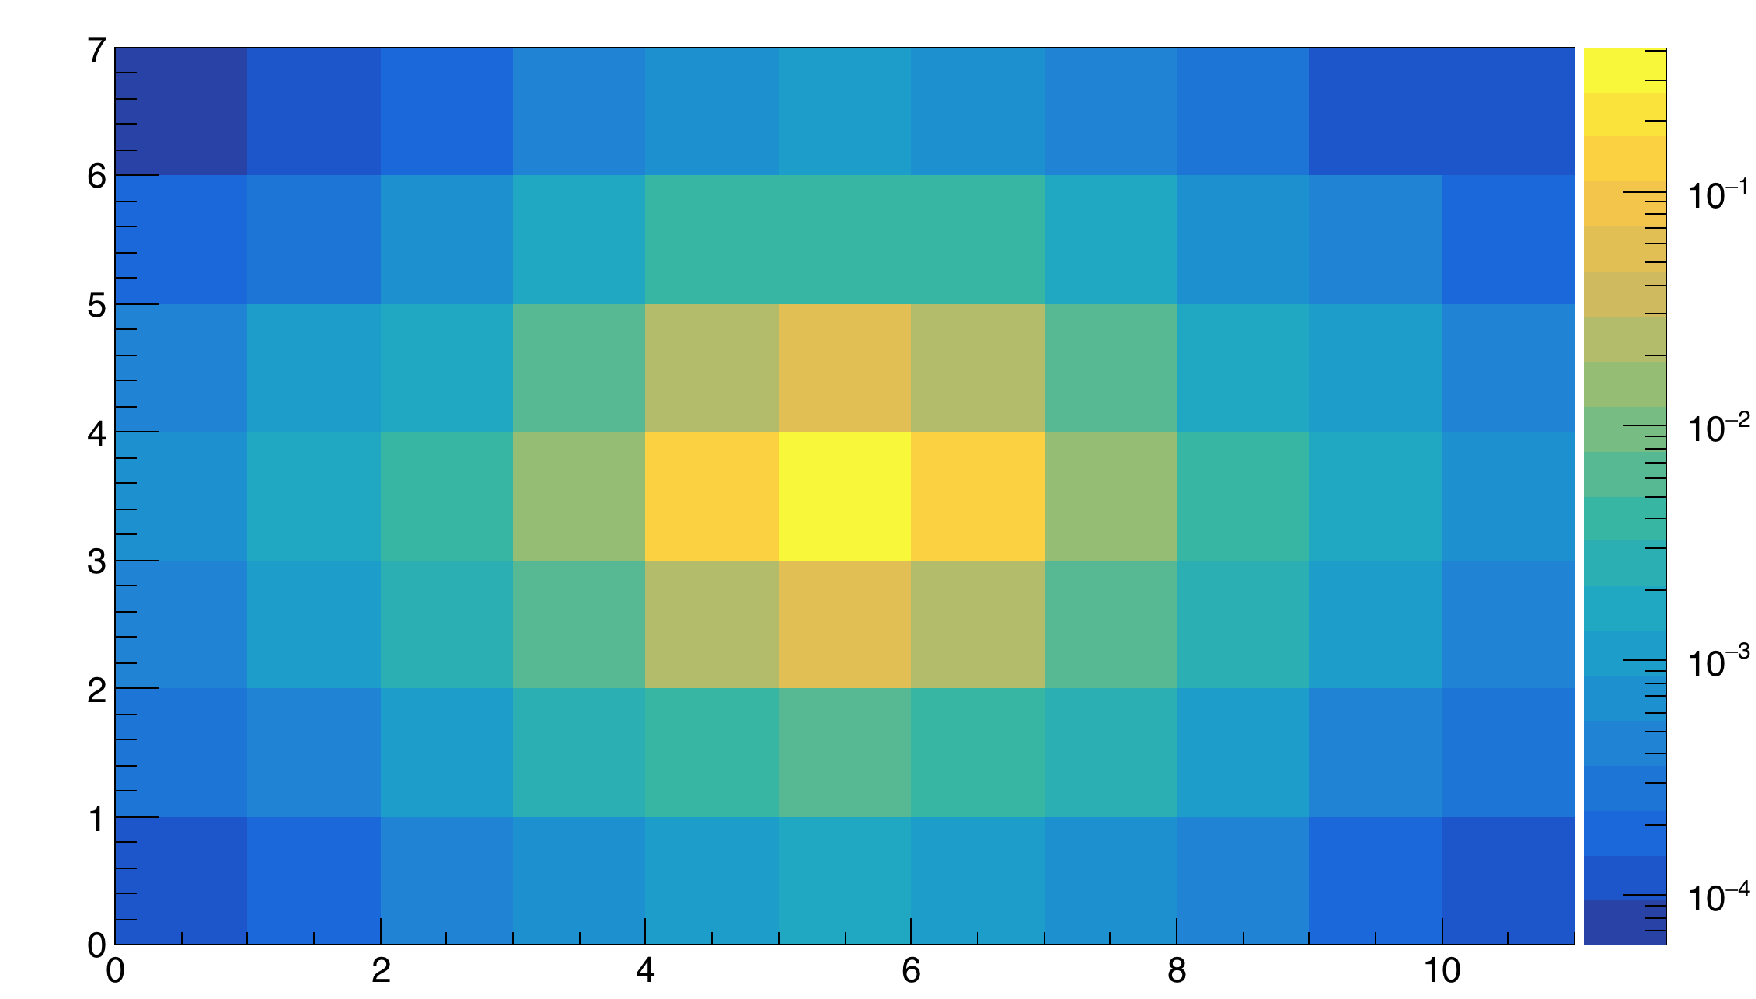
\includegraphics[width=\textwidth,keepaspectratio]{logscale.pdf}
  		\caption{Energy profile of a window of 7x11 cells in the 2nd calorimeter layer (logarithmic scale)}
  		\label{fig::profile_log}
  	\end{subfigure}
  	\hfill
  	\begin{subfigure}[t]{0.5\textwidth} 
  		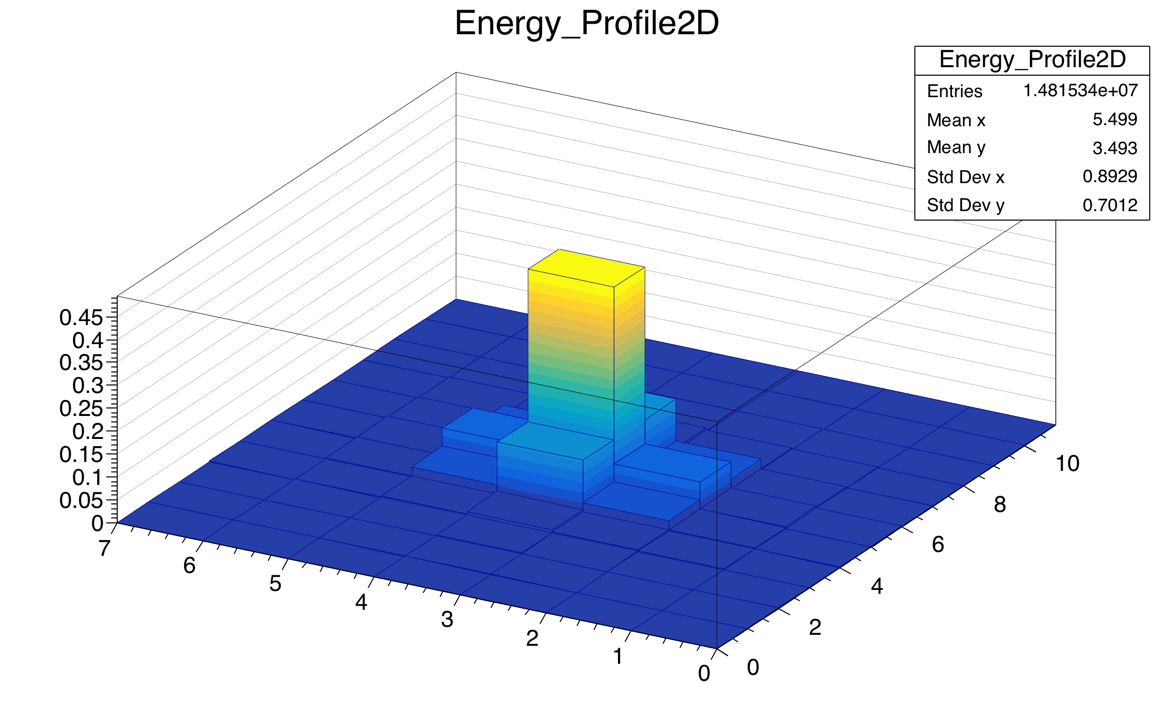
\includegraphics[width=\textwidth,keepaspectratio]{2dProfile.png}
  		\caption{2D profile of the cluster}
  		\label{fig::2d_profile}
  	\end{subfigure}
  	\caption{Visualisations of the 7x11 calorimeter cluster}
  	\label{fig::profiles}
  \end{figure}
  
  In order to characterise the energy distribution within the shower profile a number of observables called shower shapes are used. They are then used as an input for particle identification MVA algorithm. Current study focuses on the second layer of the calorimeter for which there are three shower shape observables described below \cite{egamma_perf_2017}:
  
    	\begin{figure}[htbp]
  	\begin{subfigure}[t]{0.4\textwidth}
  		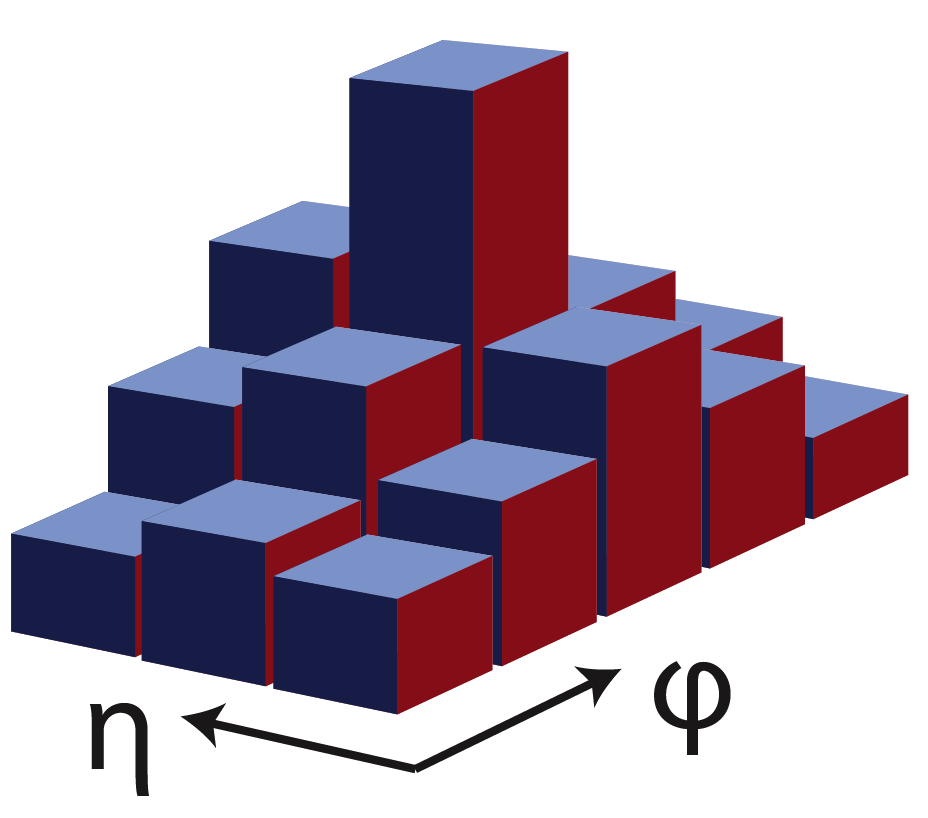
\includegraphics[width=\textwidth,keepaspectratio]{Weta2.png}
  		\caption[Lateral shower width $W_{\eta} 2$]{Lateral shower width $W_{\eta} 2$}
  		\label{fig::weta2}
  	\end{subfigure}
  	\hfill
  	\begin{subfigure}[t]{0.25\textwidth} 
  		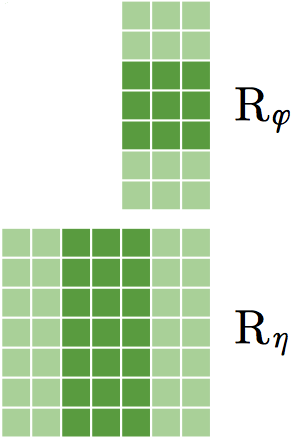
\includegraphics[width=\textwidth,keepaspectratio]{reta_rphi.png}
  		\caption[$R_{\phi}$ and $R_{\eta}$]{$R_{\phi}$ and $R_{\eta}$}
  		\label{fig::reta_rphi}
  	\end{subfigure}
  	\caption{Shower shapes in the second layer of the electromagnetic calorimeter}
  	\label{fig::sshapes}
  \end{figure}
  
  \begin{itemize}
  	\item Lateral shower width $W_{\eta 2} = \sqrt{\sum(E_i \eta^{2}_{i})-(\sum(E_i \eta_{i})/\sum(E_i))^2}$ calculated within a window of 3x5 cells.
  	\item $R_{\phi}$ - ratio of the energy in 3x3 cells over the energy in 3x7 cells centered around the hottest cell.
  	\item $R_{\eta}$ - ratio of the energy in 3x7 cells over the energy in 7x7 cells centered around the hottest cell.
  \end{itemize}
  
  The shower shapes distributions for different types of particles is shown in fig. \ref{sshapes_simul} - although the distributions overlap, combining the shower shapes information with the inputs from other detectors allow to identify the particle.  
    	\begin{figure}[htbp]
	\begin{subfigure}[t]{0.4\textwidth}
		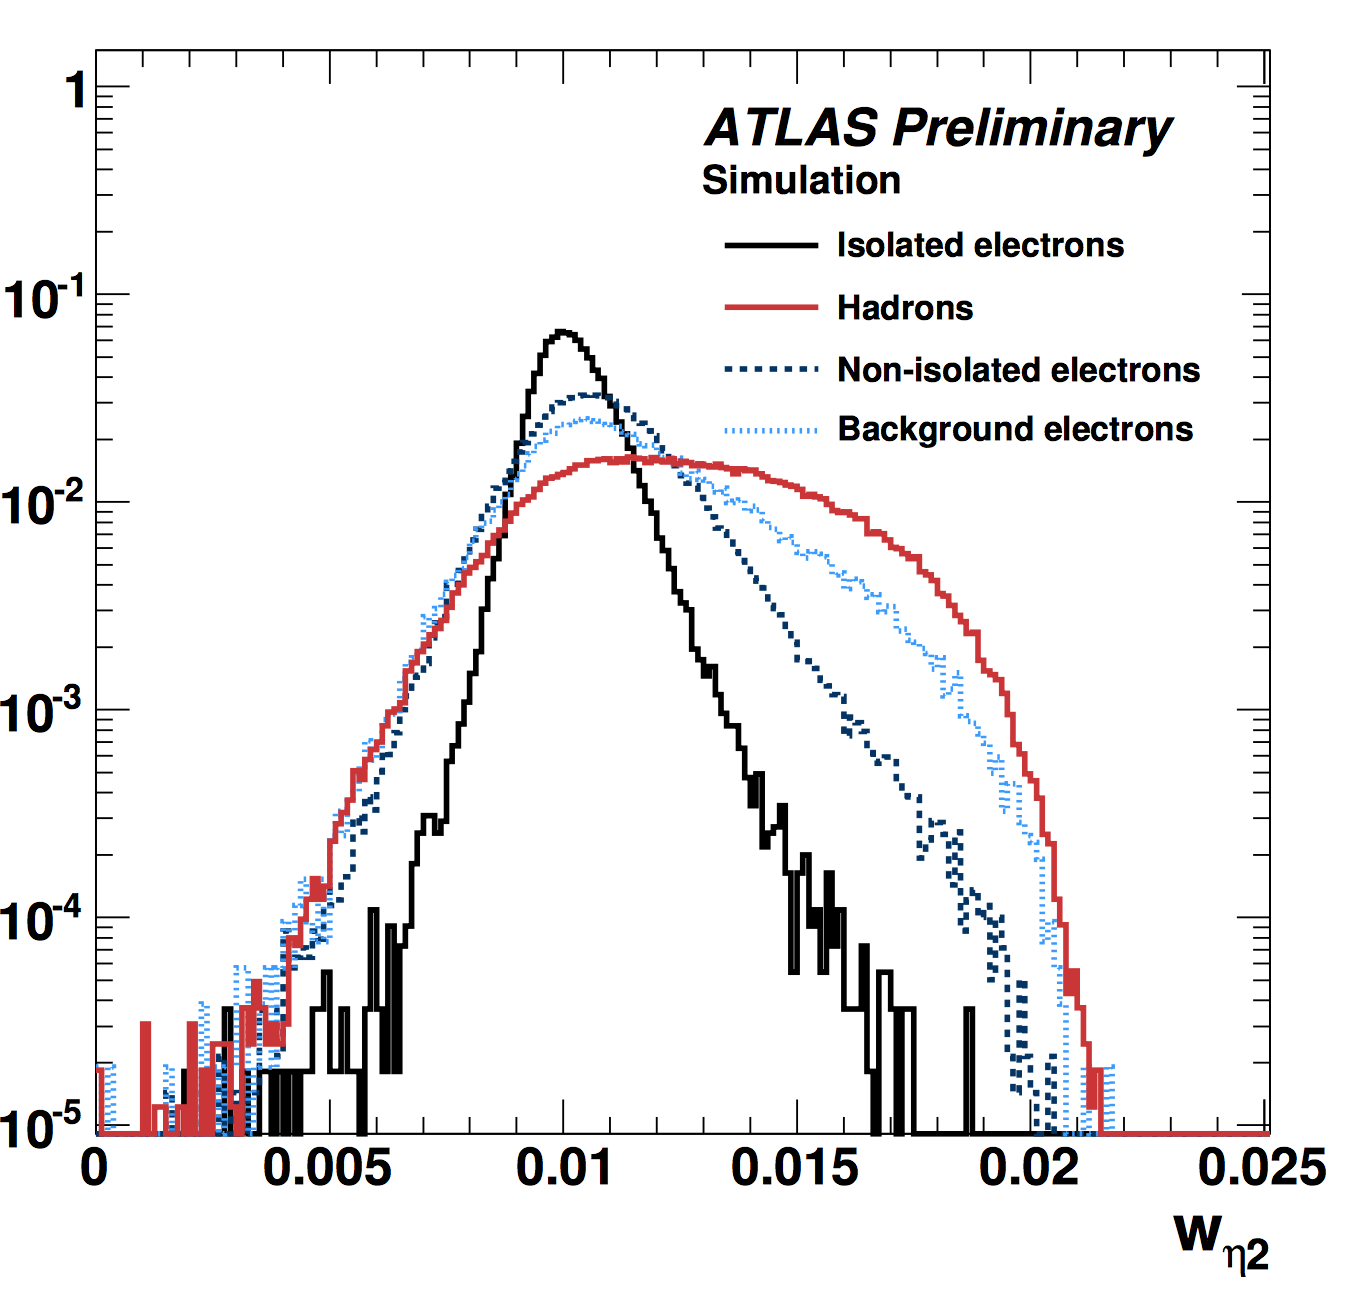
\includegraphics[width=\textwidth,keepaspectratio]{Weta2Simulation.png}
		\caption[ $W_{\eta 2}$]{$W_{\eta 2}$ distribution simulation}
		\label{fig::weta2_simul}
	\end{subfigure}
	\hfill
	\begin{subfigure}[t]{0.39\textwidth} 
		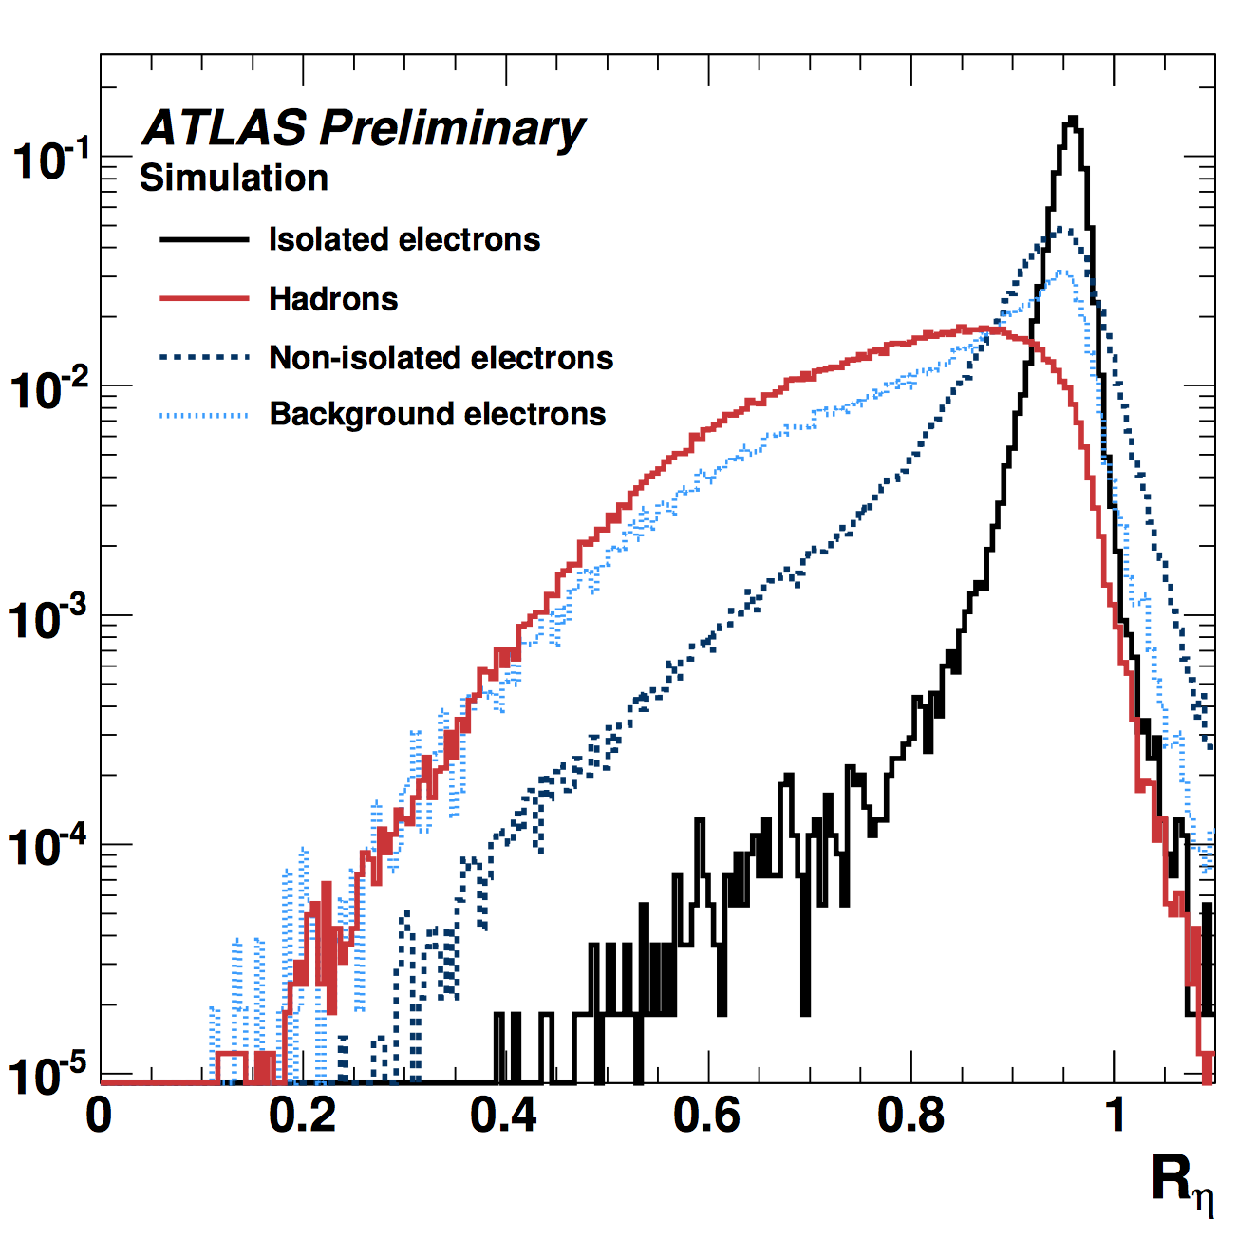
\includegraphics[width=\textwidth,keepaspectratio]{RetaSimulation.pdf}
		\caption[ $R_{\eta}$]{$R_{\eta}$ distribution simulation}
		\label{fig::reta_simul}
	\end{subfigure}
  	\caption{Distribution of $R_{\eta}$ in simulation (GEANT4) for electrons and jets \cite{sshapes_simulation}.}
	\label{fig::sshapes_simul}
\end{figure}

  Figure \ref{reta_simul} shows how $R_{\eta}$ distribution is different in jets, signal electrons and background electrons. Background electrons denote non-prompt electrons which are not originated from primary vertex. \\
 
   The shower shapes appear to be extremely sensitive to the detector material modelling. A simplification in the geometry of the EMCal absorber geometry in GEANT4 9.2 (a layered structure of the accordion was represented as a homogenous material) has lead to visible discrepancies in the shower shapes between the data and MC. This was corrected in GEANT4 9.4 significantly improving the agreement, although not eliminating it completely (see fig. \ref{fig::sshapes_geant}).  The origin for the remaining discrepancy is not clear.\\
      	\begin{figure}[htbp]
  	\begin{subfigure}[t]{0.4\textwidth}
  		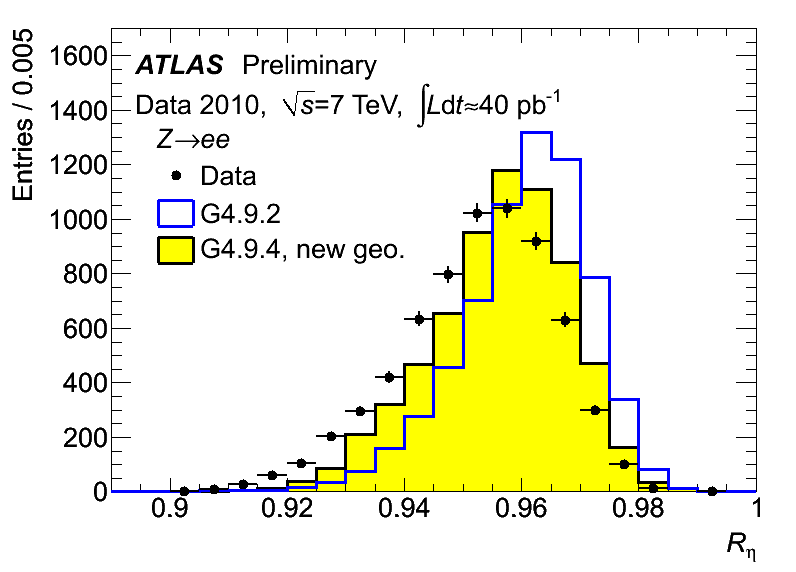
\includegraphics[width=\textwidth,keepaspectratio]{Reta_G}
  		\caption[ $W_{\eta 2}$]{$W_{\eta 2}$}
  		\label{fig::weta2_geant}
  	\end{subfigure}
  	\hfill
  	\begin{subfigure}[t]{0.4\textwidth} 
  		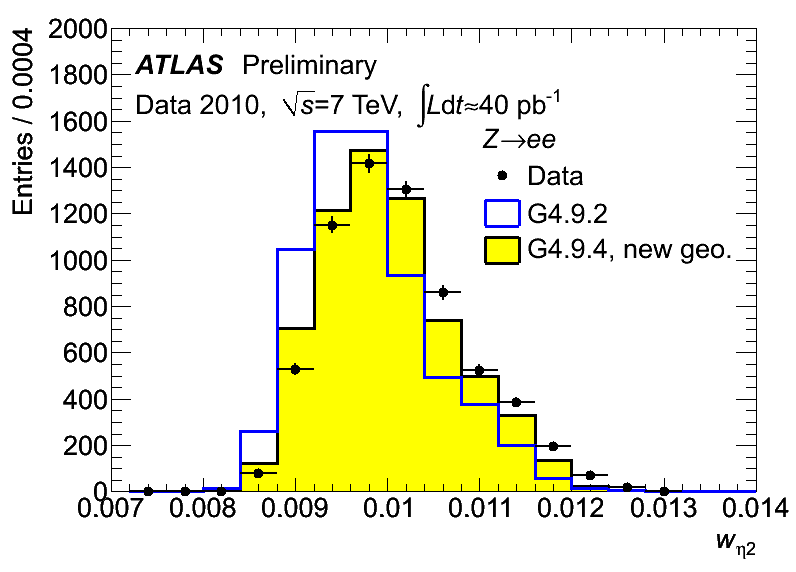
\includegraphics[width=\textwidth,keepaspectratio]{weta2_G}
  		\caption[ $R_{\eta}$]{$R_{\eta}$ }
  		\label{fig::reta_geant}
  	\end{subfigure}
  	\caption{Data/MC Comparison for Calorimeter Shower Shapes of High Et Electrons \cite{geant_corr}.}
  	\label{fig::sshapes_geant}
  \end{figure}
  
  Disagreement in shower shapes between the data and MC leads to discrepancies in particle ID which are later fixed using $\eta-$ and $p_T$-dependent scale factors. Correction of the shower shapes aims to get the scale factors closer to unity, reducing the corresponding systematic uncertainties and improving the precision of the measurements with electrons in the final states.  

  
  \section{ Shower shapes measurement and correction  }
  \subsection{Event selection}
  For this study we have considered electrons from the $Z\rightarrow ee$ decay. A set of recommended single electron triggers was used (HLT\_e26\_lhtight\_nod0\_ivarloose, HLT\_e60\_lhmedium\_nod0,\\
   HLT\_e140\_lhloose\_nod0,HLT\_e300\_etcut). Each event was required to have 2 electrons at least one of which has $p_T>25$ GeV.  In order to suppress the background both electrons had to pass gradient isolation. Z invariant mass cut was applied with a window of $80-120$GeV. To avoid identification bias from triggering the tag and probe approach was used with only probe electrons taken into consideration \cite{RecoID2011}. The electron cluster in the second calorimeter layer was required to contain information from 77 calorimeter cells. No pile-up reweighting has been applied. Datasets of 264786295 events in data (2017 proton-proton collisions) and 79340000 events in MC (Powheg+Pythia8) were used. 
  \subsection{Data/MC discrepancies}
  Our consideration begins with the energy deposit of an electron in the second layer of the calorimeter. A window of 7 cells in $\eta$ and 11 cells in $\phi$ is centered around the cell with the highest energy.

  Shower shapes were considered in 14 $\eta$ bins in the range between $|\eta| = (0,2.4)$ in order to investigate how the discrepancy depends on $\eta$. 
    	\begin{figure}[htbp]
  	\begin{subfigure}[t]{0.5\textwidth}
  		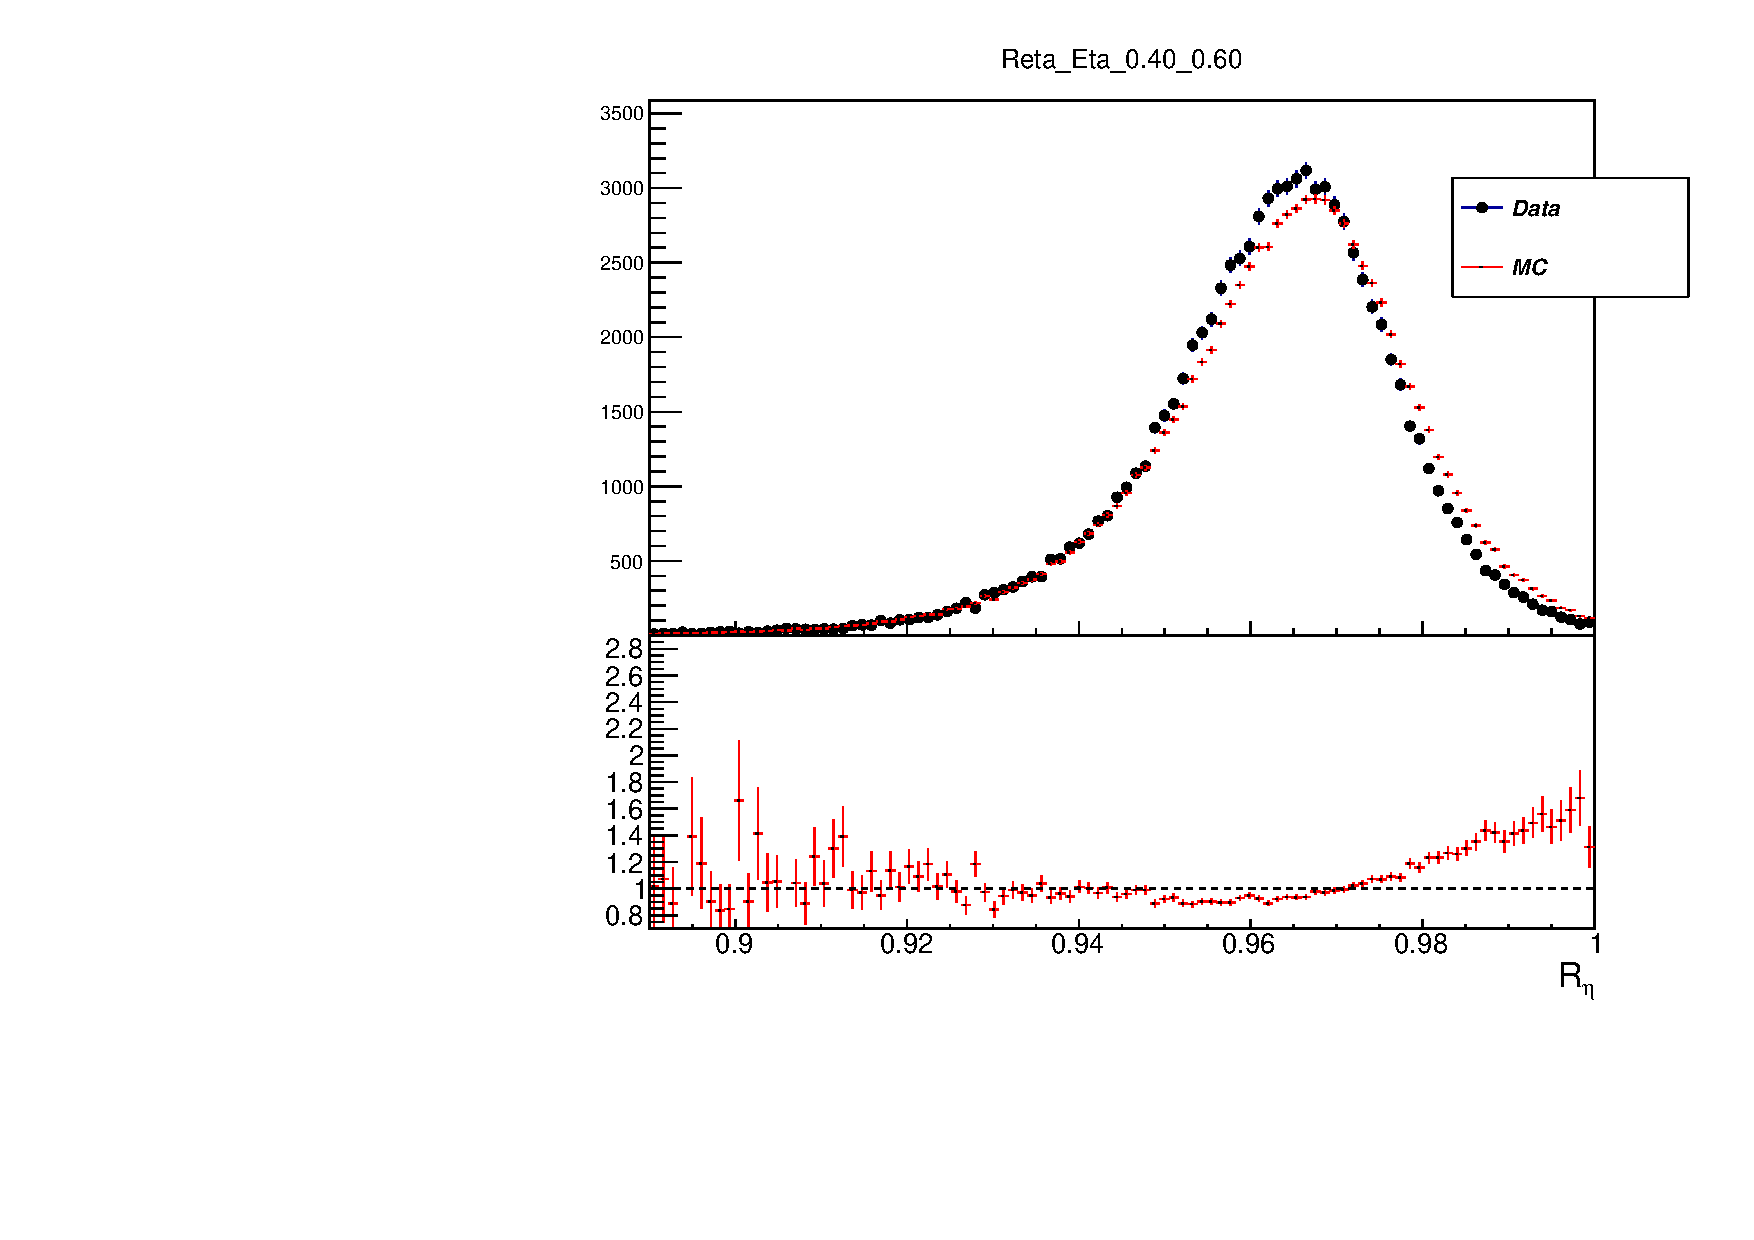
\includegraphics[width=\textwidth,keepaspectratio]{Reta2_Eta_4_6.pdf}
  		\caption{$R_{\eta}$ in $|\eta| = (0.4,0.6)$ }
  		\label{fig::reta_norew_04}
  	\end{subfigure}
  	\hfill
  	\begin{subfigure}[t]{0.5\textwidth} 
  		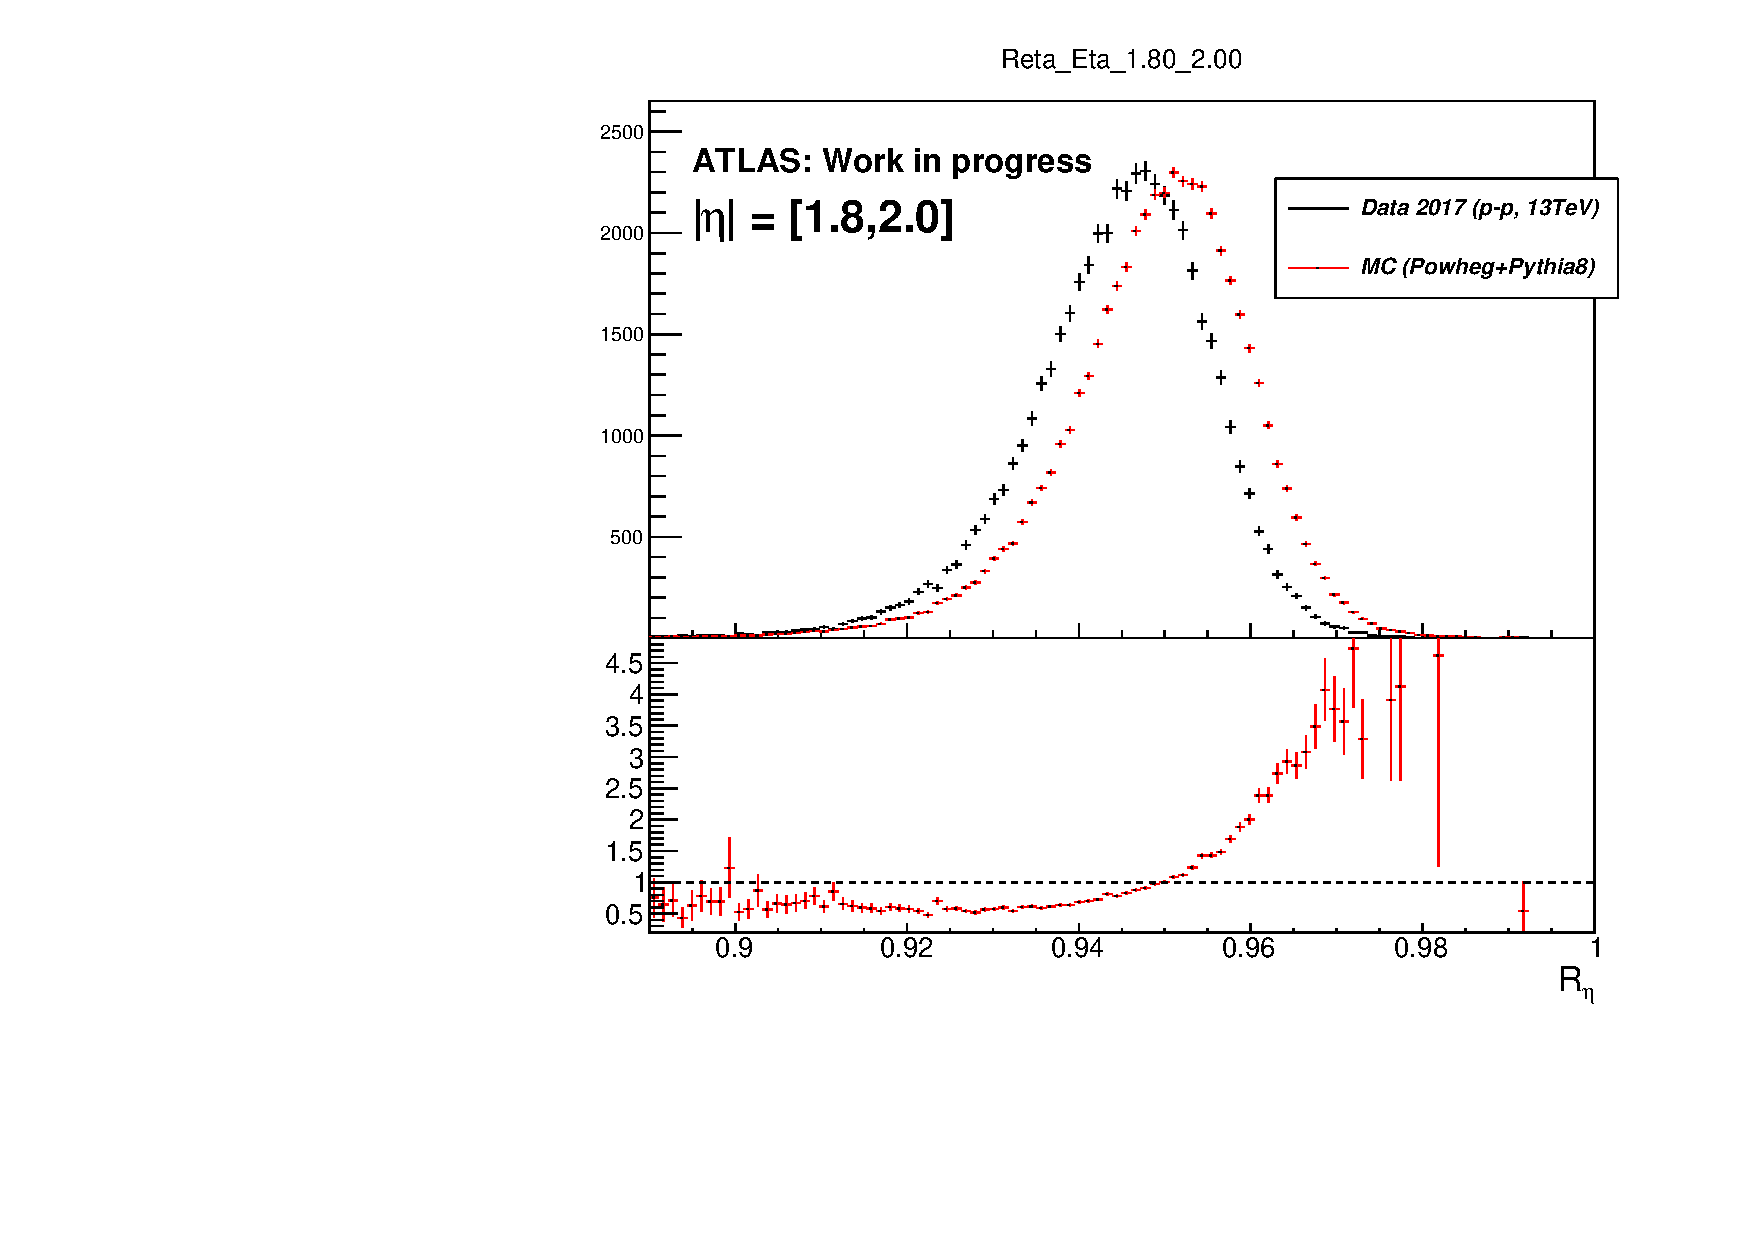
\includegraphics[width=\textwidth,keepaspectratio]{Reta2_Eta_18_20.pdf}
  		\caption{$R_{\eta}$ in $|\eta| = (1.8,2.0)$ }
  		\label{fig::reta_norew_18}
  	\end{subfigure}
  	\caption{$R_{\eta}$ in the barel and in the end-cap, Data vs MC}
  	\label{fig::reta_norew}
  \end{figure}

    \begin{figure}[htbp]
	\begin{subfigure}[t]{0.5\textwidth}
		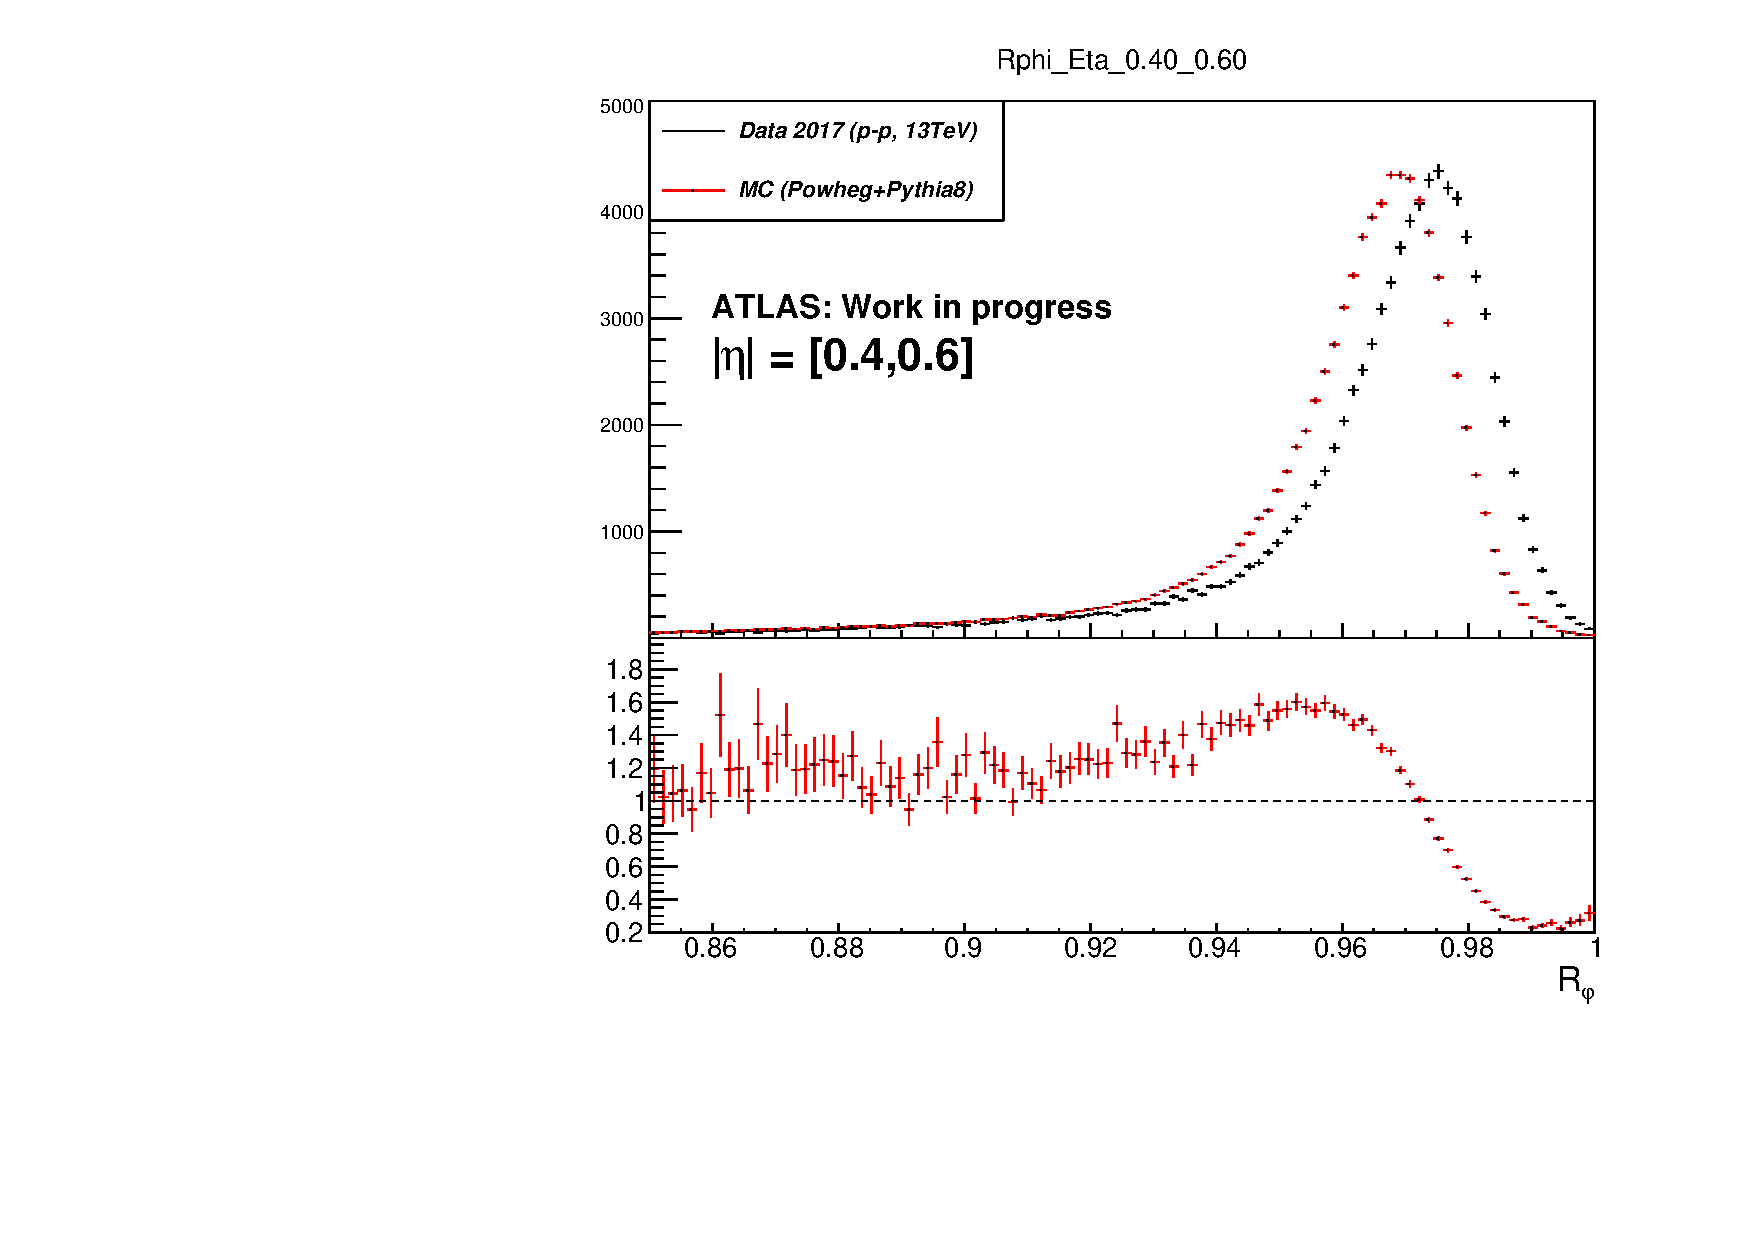
\includegraphics[width=\textwidth,keepaspectratio]{Rphi2_Eta_4_6.pdf}
		\caption{$R_{\phi}$ in $|\eta| = (0.4,0.6)$ }
		\label{fig::rphi_norew_04}
	\end{subfigure}
	\hfill
	\begin{subfigure}[t]{0.5\textwidth} 
		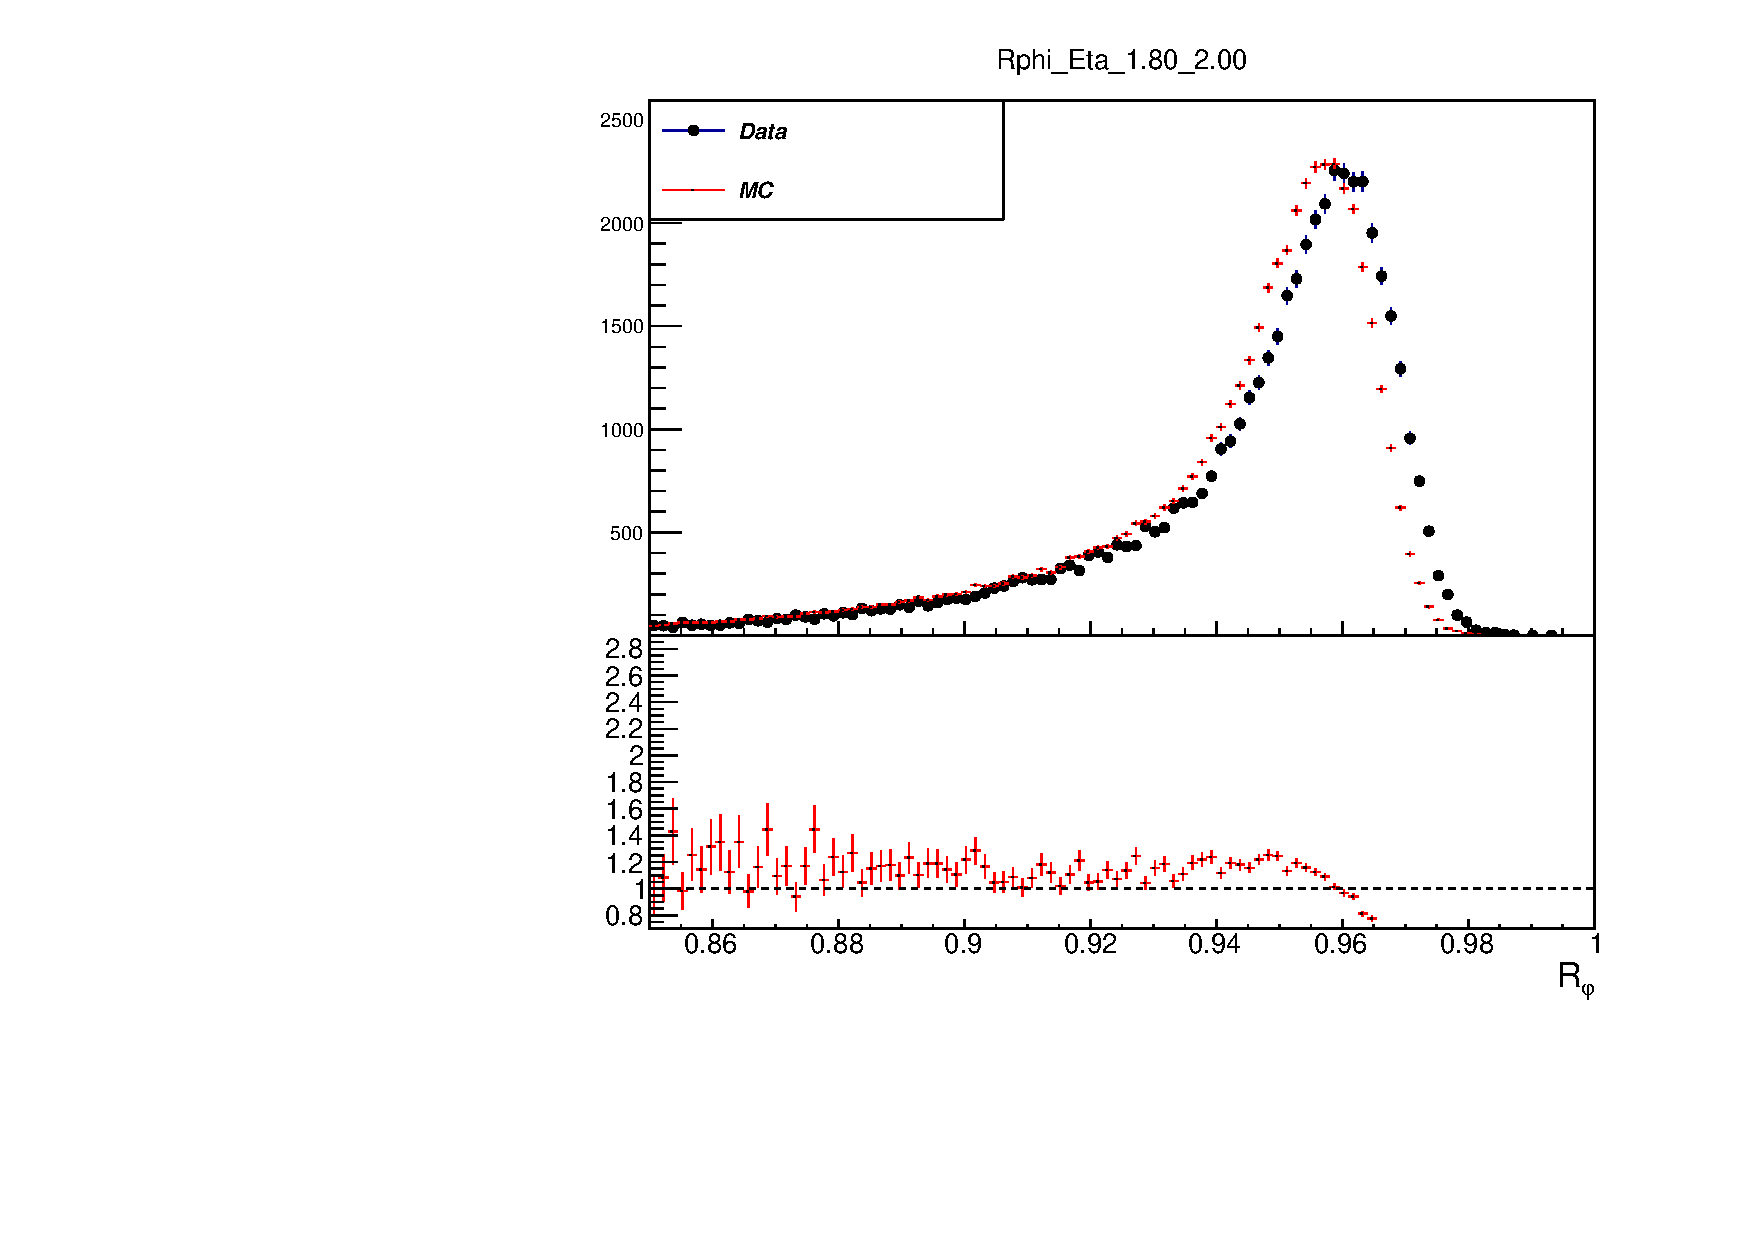
\includegraphics[width=\textwidth,keepaspectratio]{Rphi2_Eta_18_20.pdf}
		\caption{$R_{\phi}$ in $|\eta| = (1.8,2.0)$ }
		\label{fig::rphi_norew_18}
	\end{subfigure}
	\caption{$R_{\phi}$ in the barel and in the end-cap, Data vs MC}
	\label{fig::rphi_norew}
\end{figure}
  
    \begin{figure}[htbp]
	\begin{subfigure}[t]{0.5\textwidth}
		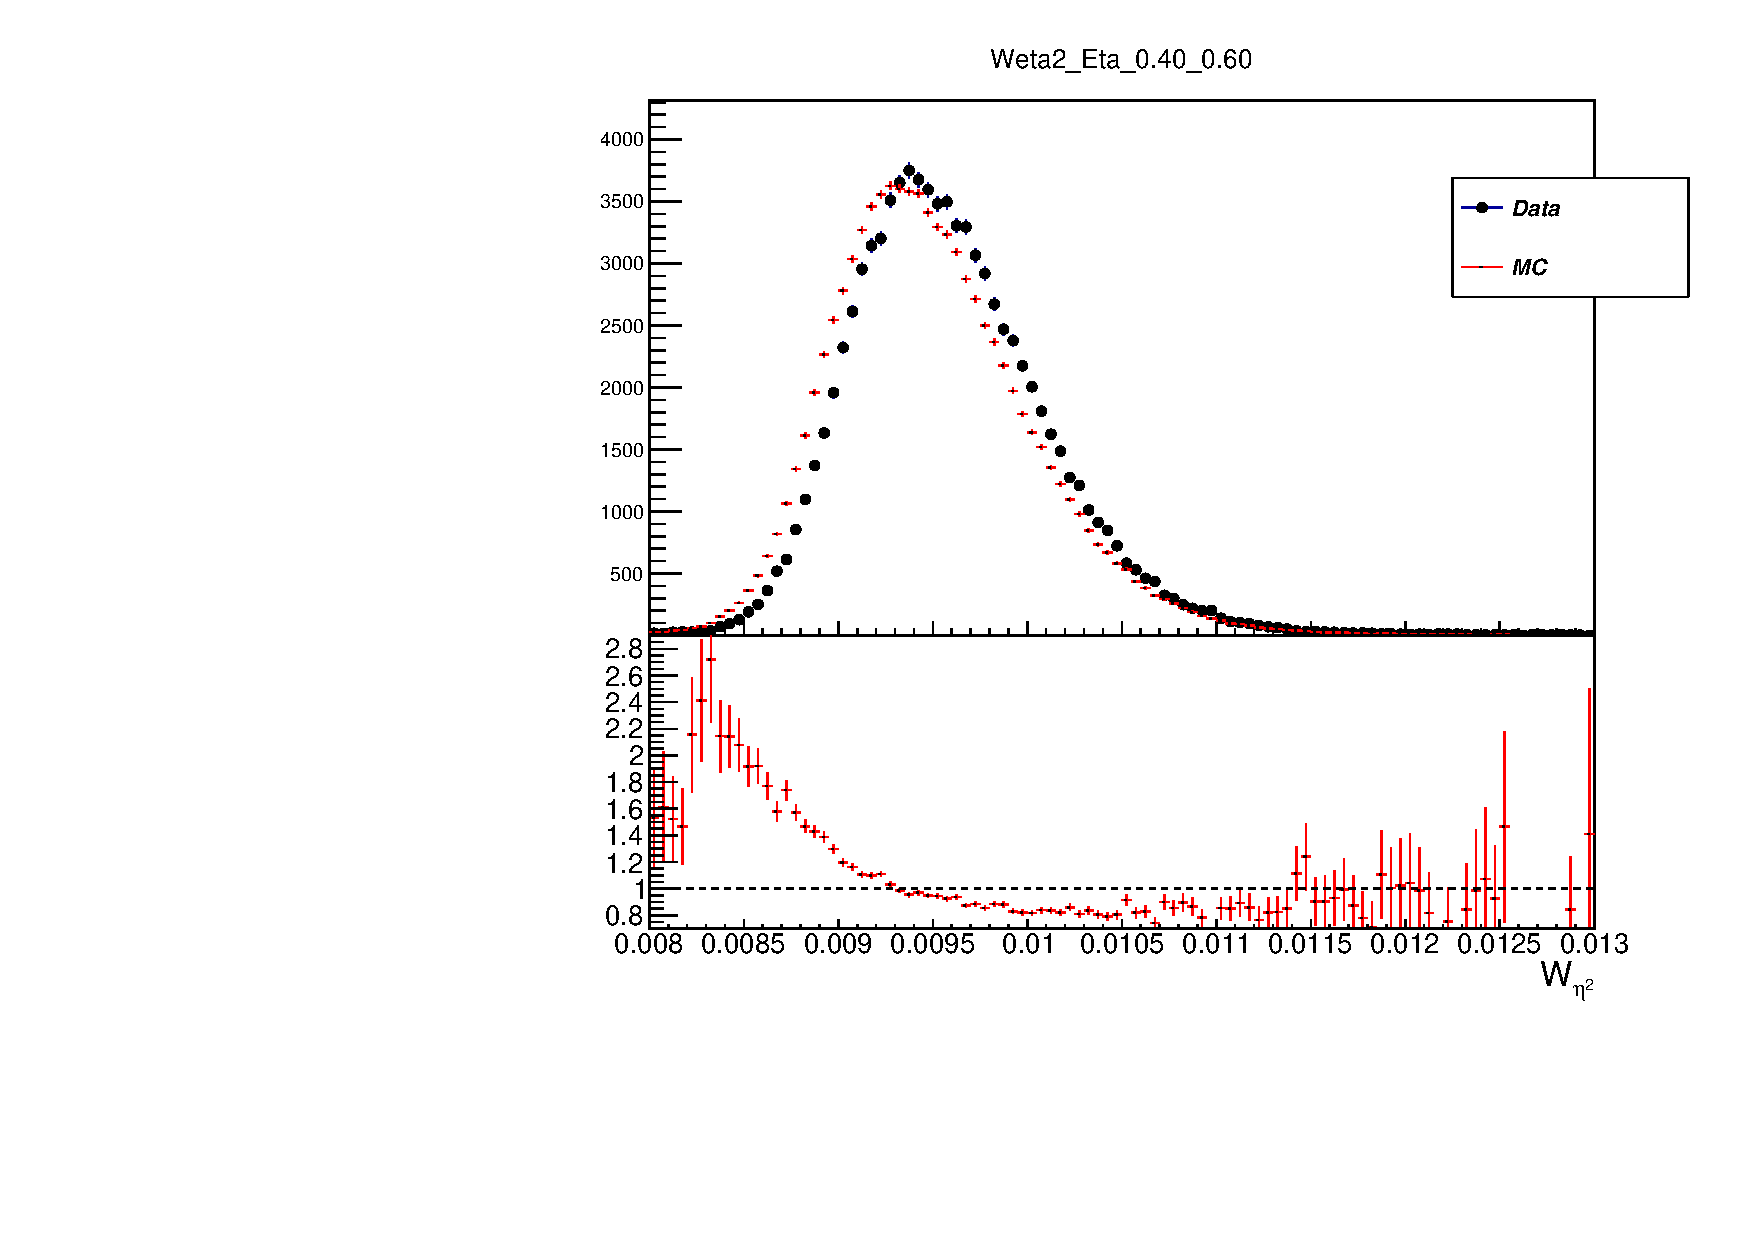
\includegraphics[width=\textwidth,keepaspectratio]{weta22_Eta_4_6.pdf}
		\caption{$W_{\eta}^2$ in $|\eta| = (0.4,0.6)$ }
		\label{fig::weta2_norew_04}
	\end{subfigure}
	\hfill
	\begin{subfigure}[t]{0.5\textwidth} 
		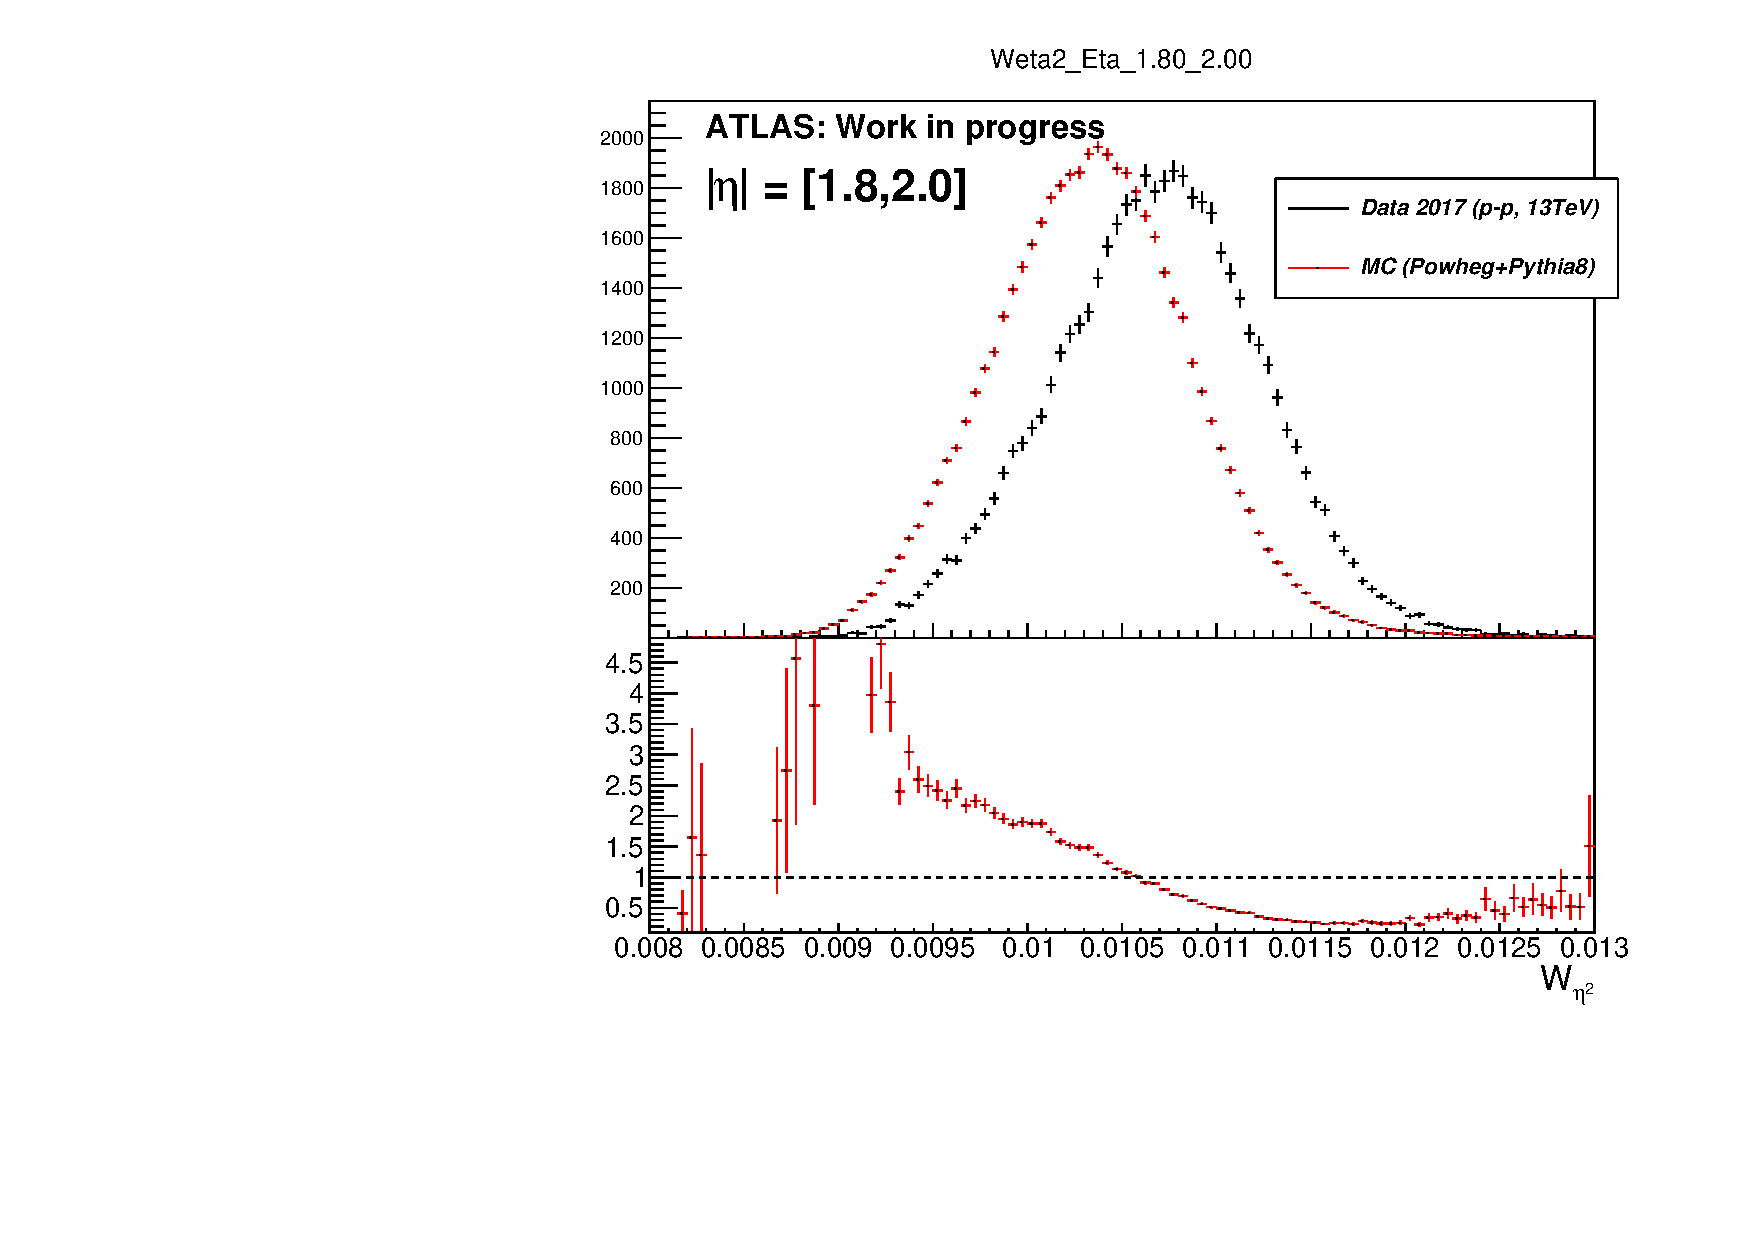
\includegraphics[width=\textwidth,keepaspectratio]{weta22_Eta_18_20.pdf}
		\caption{$W_{\eta}^2$ in $|\eta| = (1.8,2.0)$ }
		\label{fig::weta2_norew_18}
	\end{subfigure}
	\caption{$W_{\eta}^2$ in the barel and in the end-cap, Data vs MC}
	\label{fig::weta2_norew}
\end{figure}



  The $\eta$-dependent shower shapes in data are wider than the MC and show a larger discrepancy in the endcap ($|\eta| = (1.52,2.4)$). For $\phi$ dimension the situation is the opposite: MC is wider than the data and the barrel ($|\eta| = (0,1.52)$) shows larger discrepancy. Figures \ref{Reta2}, \ref{Rphi2}, \ref{Weta22} contain examples of shower shapes in different eta bins. 
  \subsection{The correction procedure}
  \subsubsection{The correction matrix}
  The correction procedure is based on the redistribution of energy between the cluster cells in MC so that the distribution becomes consistent with the data. For every $\eta$ bin a correction matrix is derived in the following way:
  \begin{equation}
  \nonumber
  \large {M_{i}^{Correction} = \frac{E_{i}^{Data}}{\Sigma E^{Data}} - \frac{E_{i}^{MC}}{\Sigma E^{MC}}}
  \end{equation}
  $\Sigma_i M_i^{Correction} = 0$, $i = 1..77$.\\
  $E_i^{Data}$, $E_i^{MC}$ - matrix elements of the averaged energy profiles. 
  The correction is then applied to the electron cluster cells on event-by-event basis:
  \begin{equation}
  \nonumber
  \large {E_{i}^{Reweighted} = {E_{i}^{Non-reweighted}(1+M_{i}^{Correction}).}}
  \end{equation}
  This redistributes the energy among the cells keeping the total energy exactly the same.
  \subsubsection{Bremsstrahlung tails}
  The magnetic field directed along the $\phi$ dimension leads to a significant asymmetry in energy deposits for electrons and positrons (figure \ref{chargeAsym}). 
  
  
      \begin{figure}[htbp]
  	\begin{subfigure}[t]{0.5\textwidth}
  		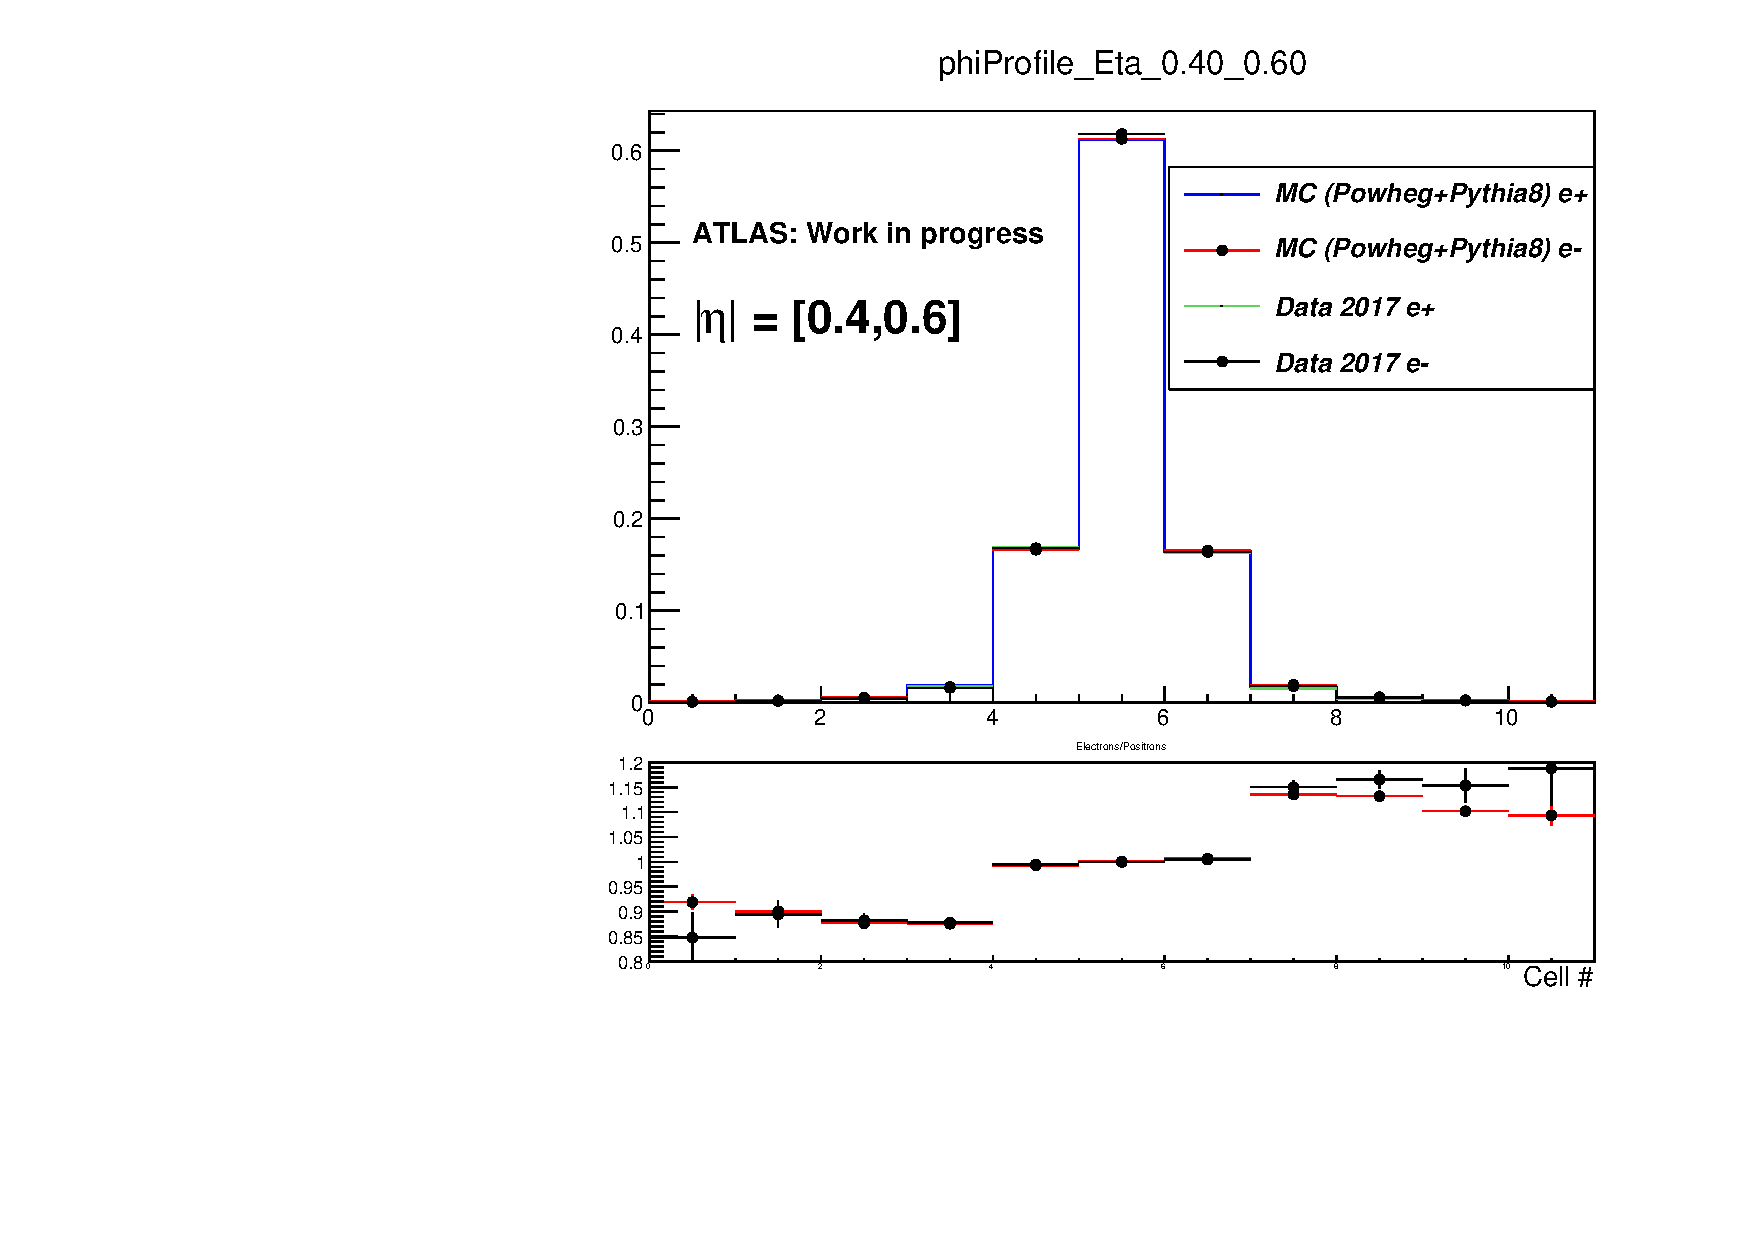
\includegraphics[width=\textwidth,keepaspectratio]{phiProfileDataMC_Eta_4_6.pdf}
  		\caption{$R_{\phi}$ in $|\eta| = (0.4,0.6)$ }
  		\label{fig::rphi_norew_04}
  	\end{subfigure}
  	\hfill
  	\begin{subfigure}[t]{0.5\textwidth} 
  		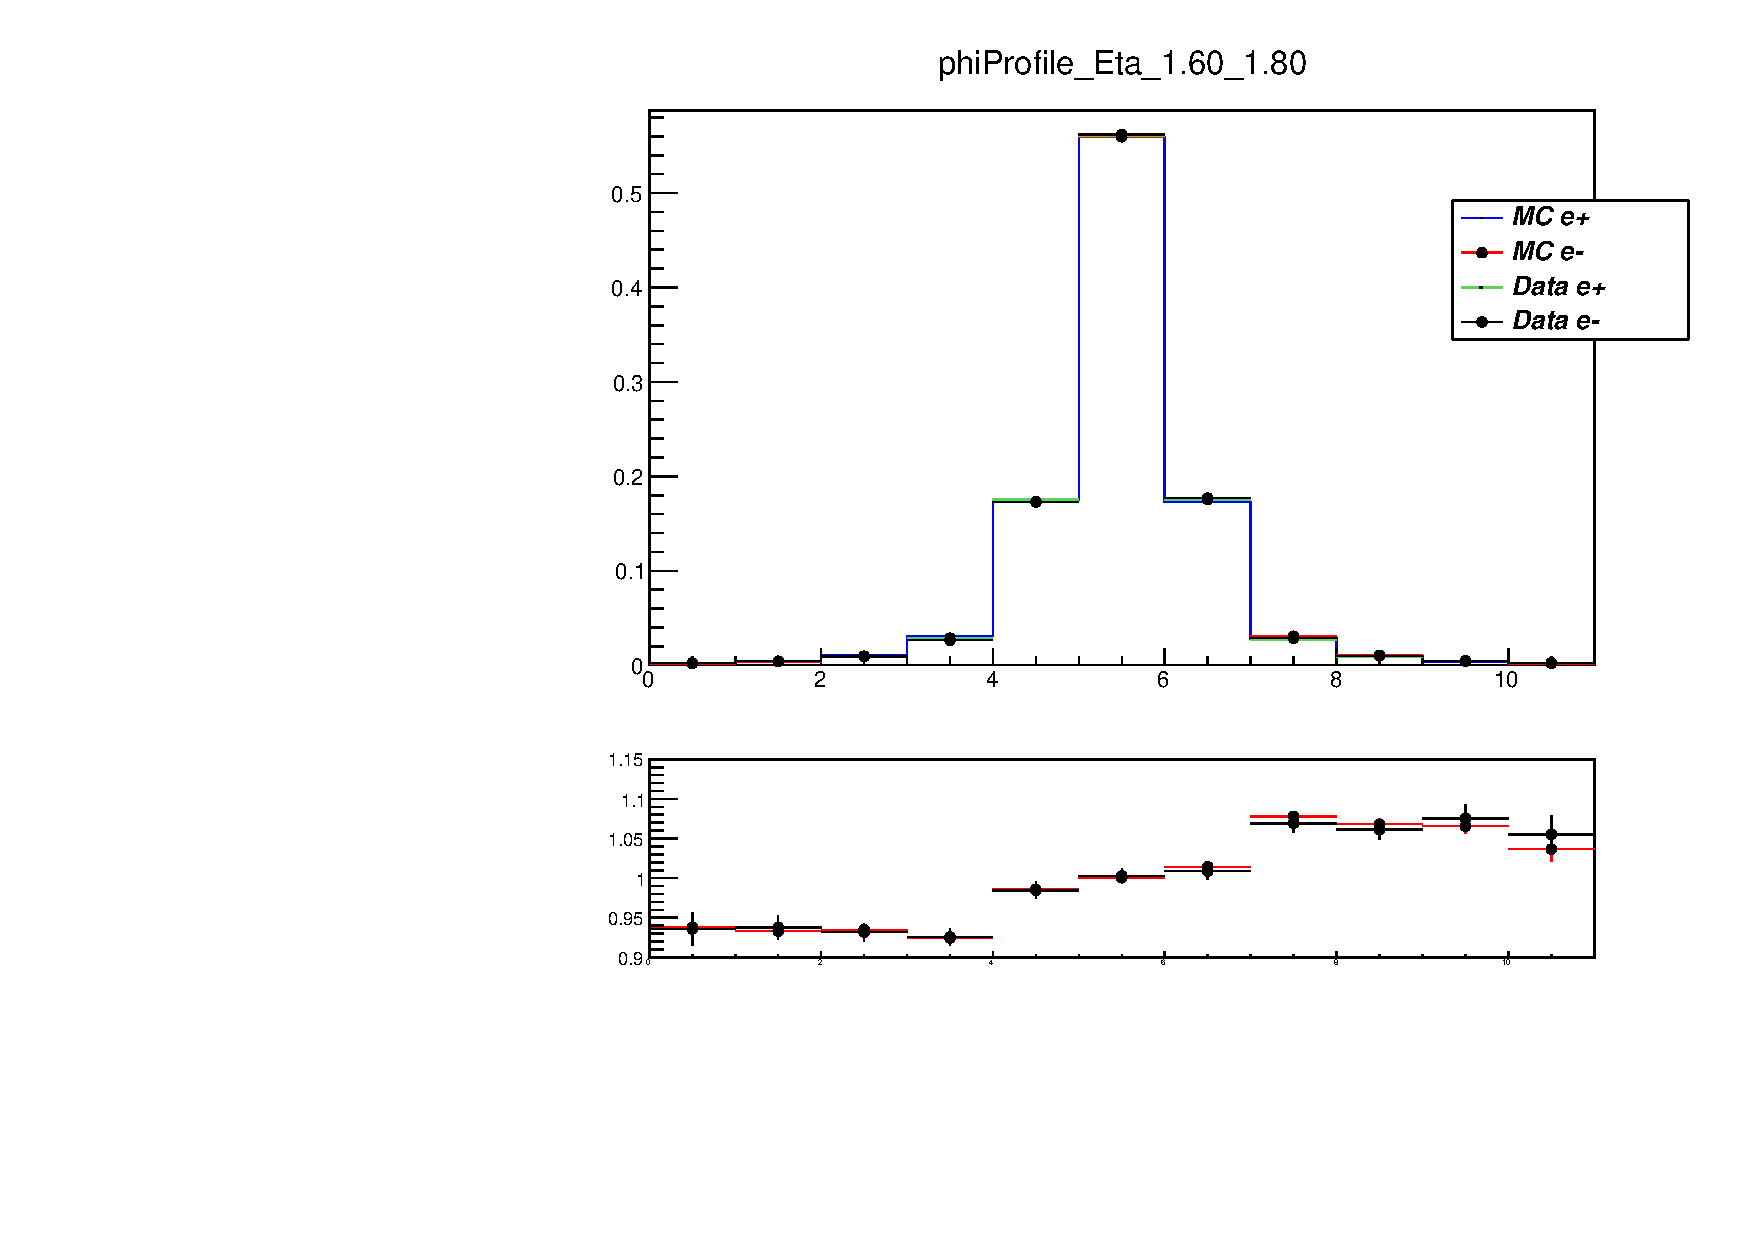
\includegraphics[width=\textwidth,keepaspectratio]{phiProfileDataMC_Eta_16_18.pdf}
  		\caption{$R_{\phi}$ in $|\eta| = (1.8,2.0)$ }
  		\label{fig::rphi_norew_18}
  	\end{subfigure}
  	\caption{$R_{\phi}$ in the barel and in the end-cap, Data vs MC}
  	\label{fig::rphi_norew}
  \end{figure}

  
  Considering the fact that the reweighting is intended to correct for the data/MC discrepancies themselves and not for the bremsstrahlung effect it makes sense to develop the bremsstrahlung-free correction function based on $e^+$ and $e^-$ correction matrices. The principle is schematically explained on figure \ref{bstails}.\\
  \begin{figure}[htbp]
  	\begin{center}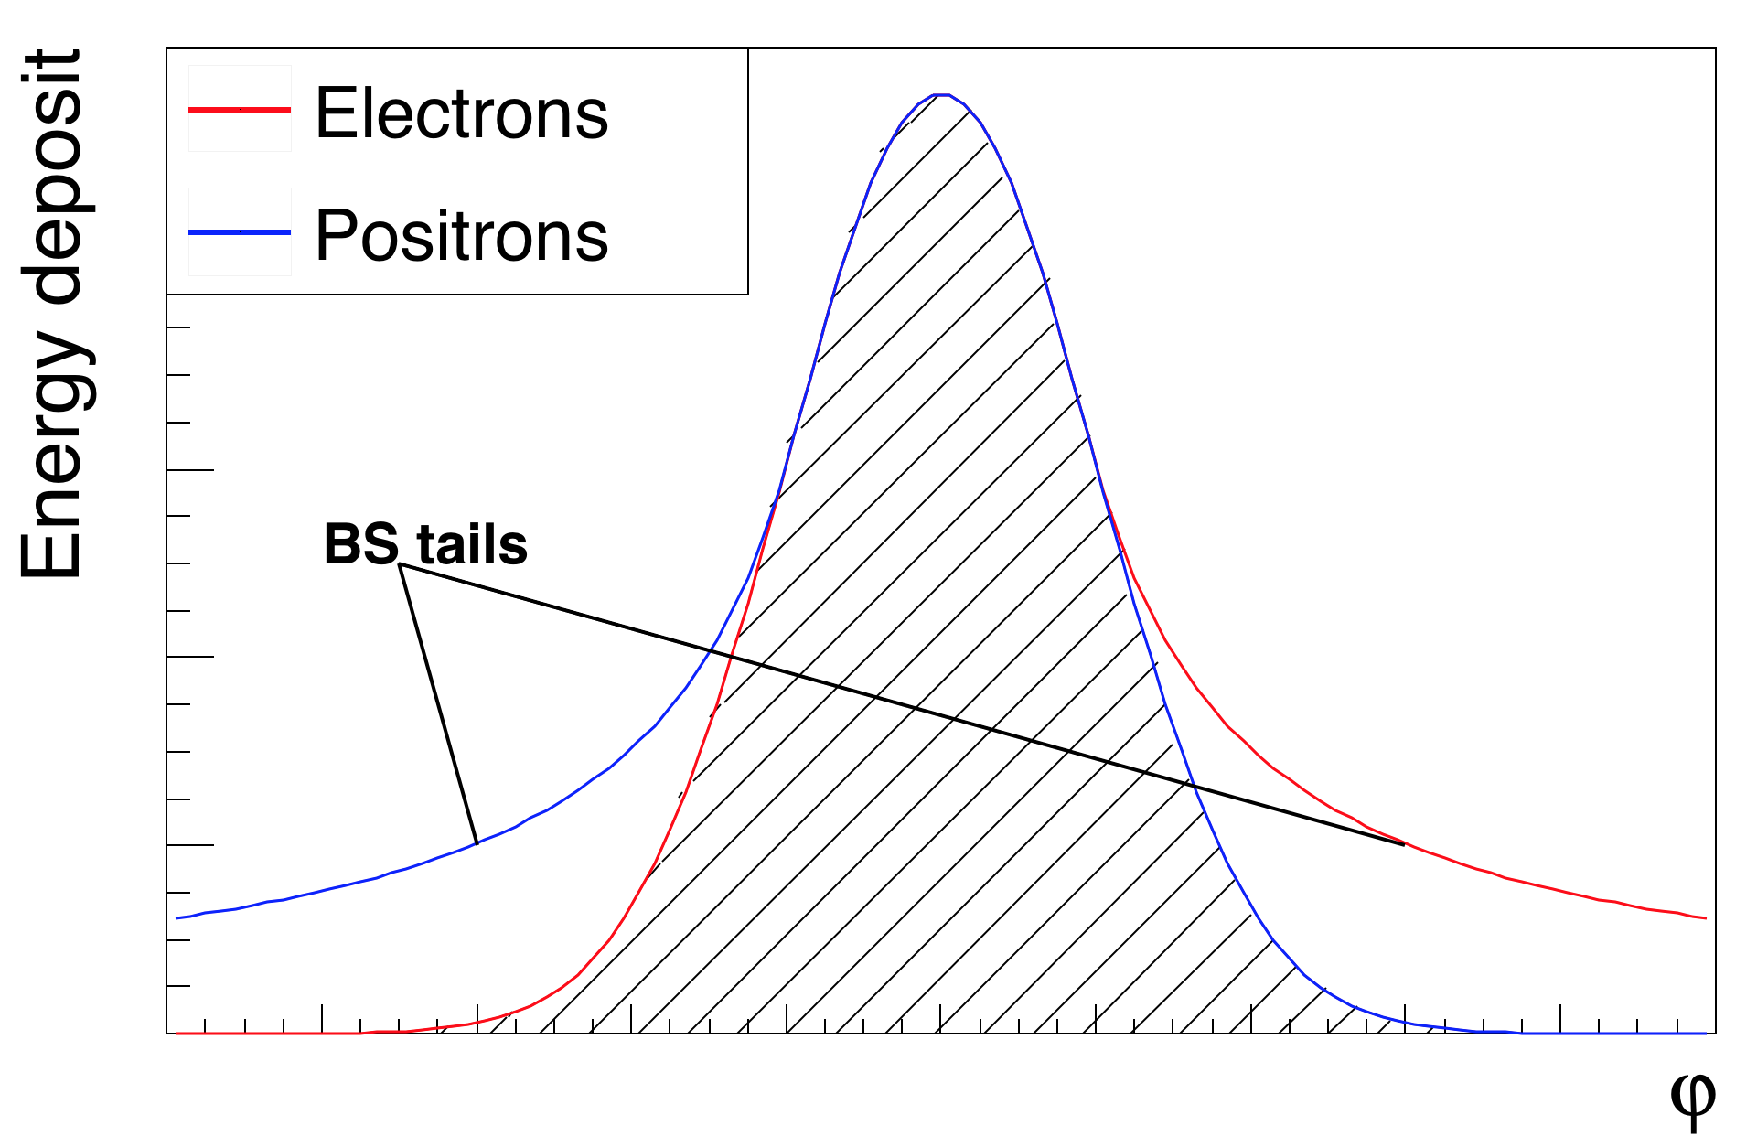
\includegraphics[%
  		width=7cm,
  		keepaspectratio]{bs_tails.pdf}\end{center}
  	\caption{Schematic energy profile in $\phi$ dimension. Bremsstrahlung tails subtraction based on $e^+$ and $e^-$ energy profiles.}
  	\label{bstails}
  \end{figure}
  Good agreement of data and MC description of $e^+$ and $e^-$ asymmetry gives a hint that the material mismodelling cannot be the main source of the data/MC disagreement.\\
  
  \section{Results}
  Figures \ref{fig::reta}, \ref{fig::rphi_rew}, \ref{fig::weta2_rew} show the effect of the correction. The shower shapes in MC become very close to the data, correcting a significant discrepancy. \\
  Figures \ref{fig::integrated} contain shower shapes vs $p_T$ integrated over $\eta$. They demonstrate that the correction does not depend on the $p_T$ which allows to expect the decreased systematic uncertainties for $p_T$ regions distant from $40-50$GeV.\\
  Finally, figure \ref{SF} shows the effect of the correction on electron ID efficiency. We can see a visible improvement, notably in the endcap region.
  Nevertheless the barrel region shows little improvement. It can be explained by the fact that electron ID MVA relies on many variables while only a number of them were corrected during current study.\\
  The proposed method is getting integrated into ATLAS Athena framework as an option and is planned to be used as a baseline for Run 3. 
  
  	\begin{figure}[htbp]
  	\begin{subfigure}[t]{0.5\textwidth}
  		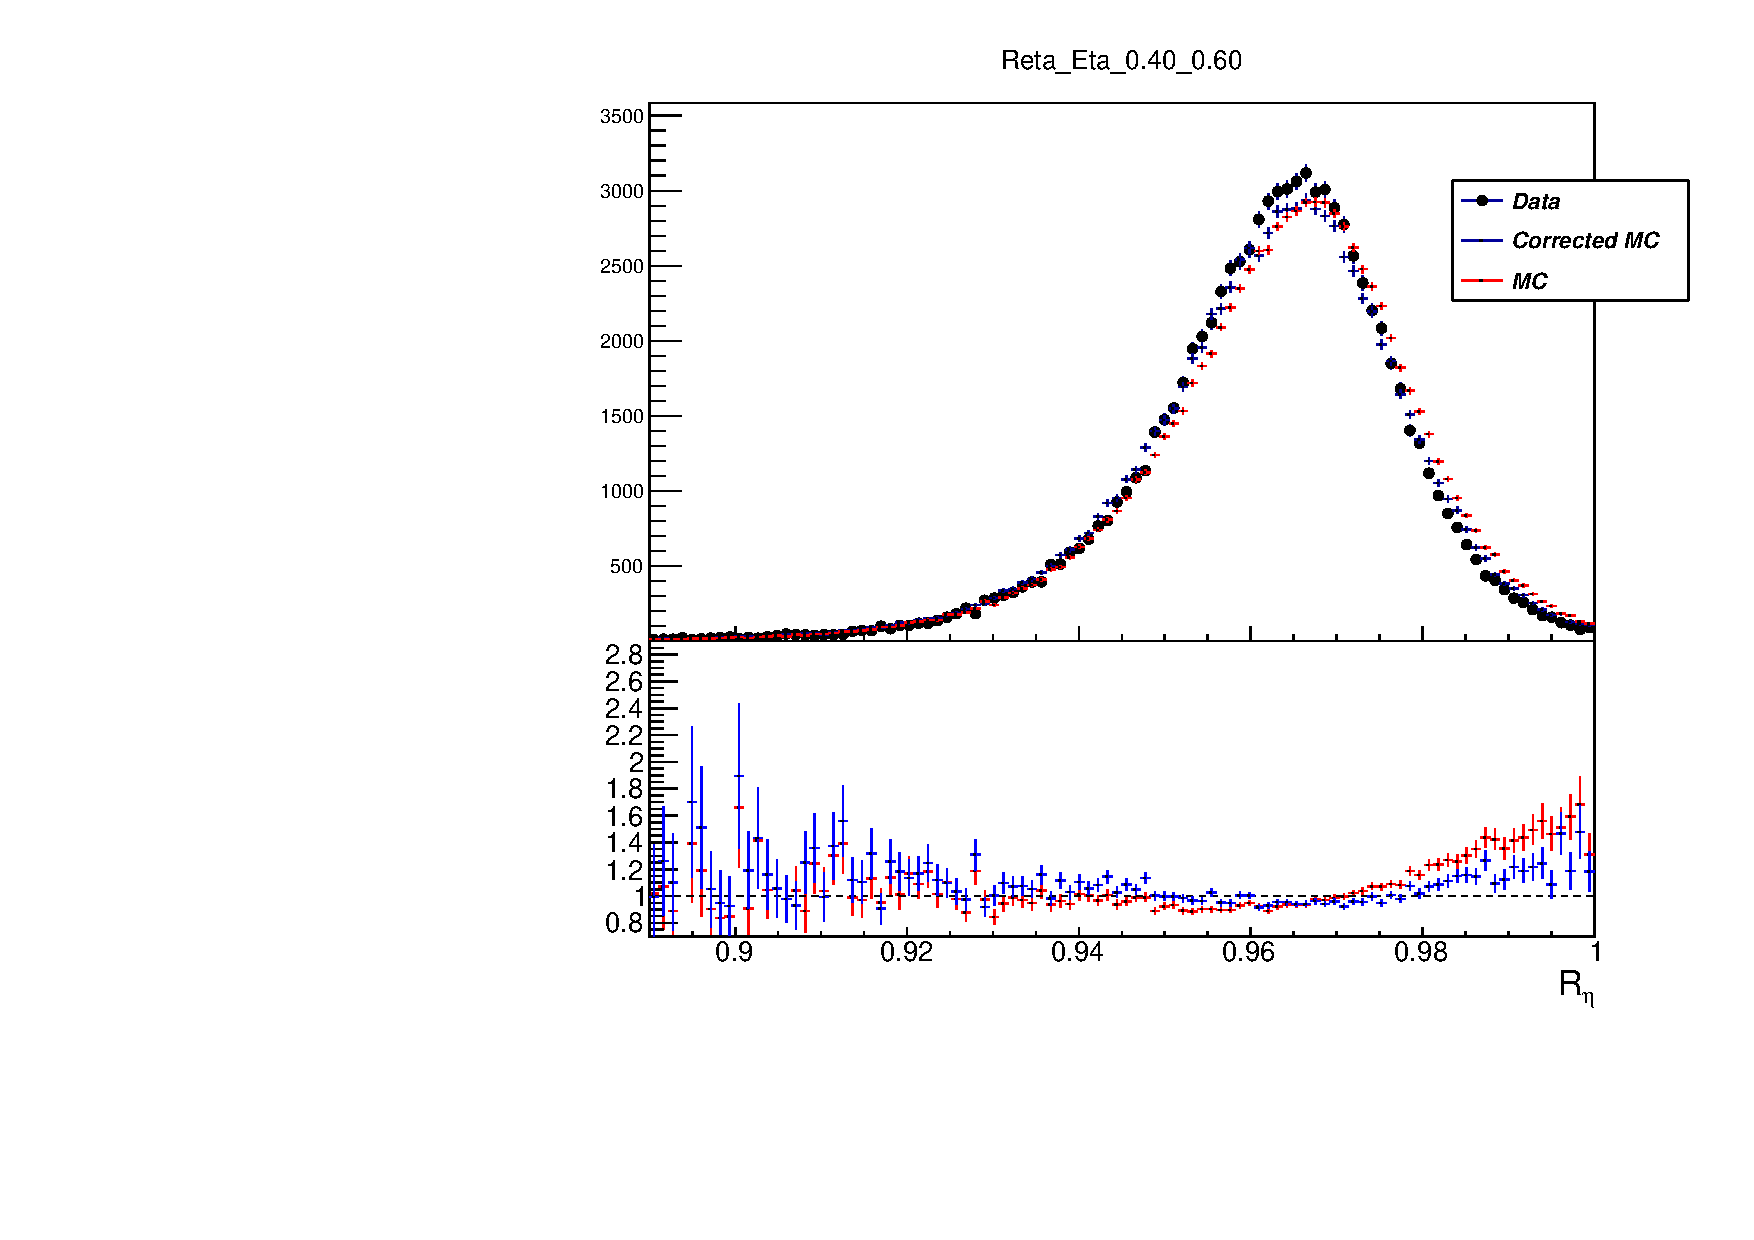
\includegraphics[width=\textwidth,keepaspectratio]{Reta_Eta_4_6_Athena.pdf}
  		\caption{Reweighted  $R_{\eta }$ in $|\eta| = (0.4,0.6)$.  }
  		\label{fig::id}
  	\end{subfigure}
  	\hfill
  	\begin{subfigure}[t]{0.5\textwidth} 
  		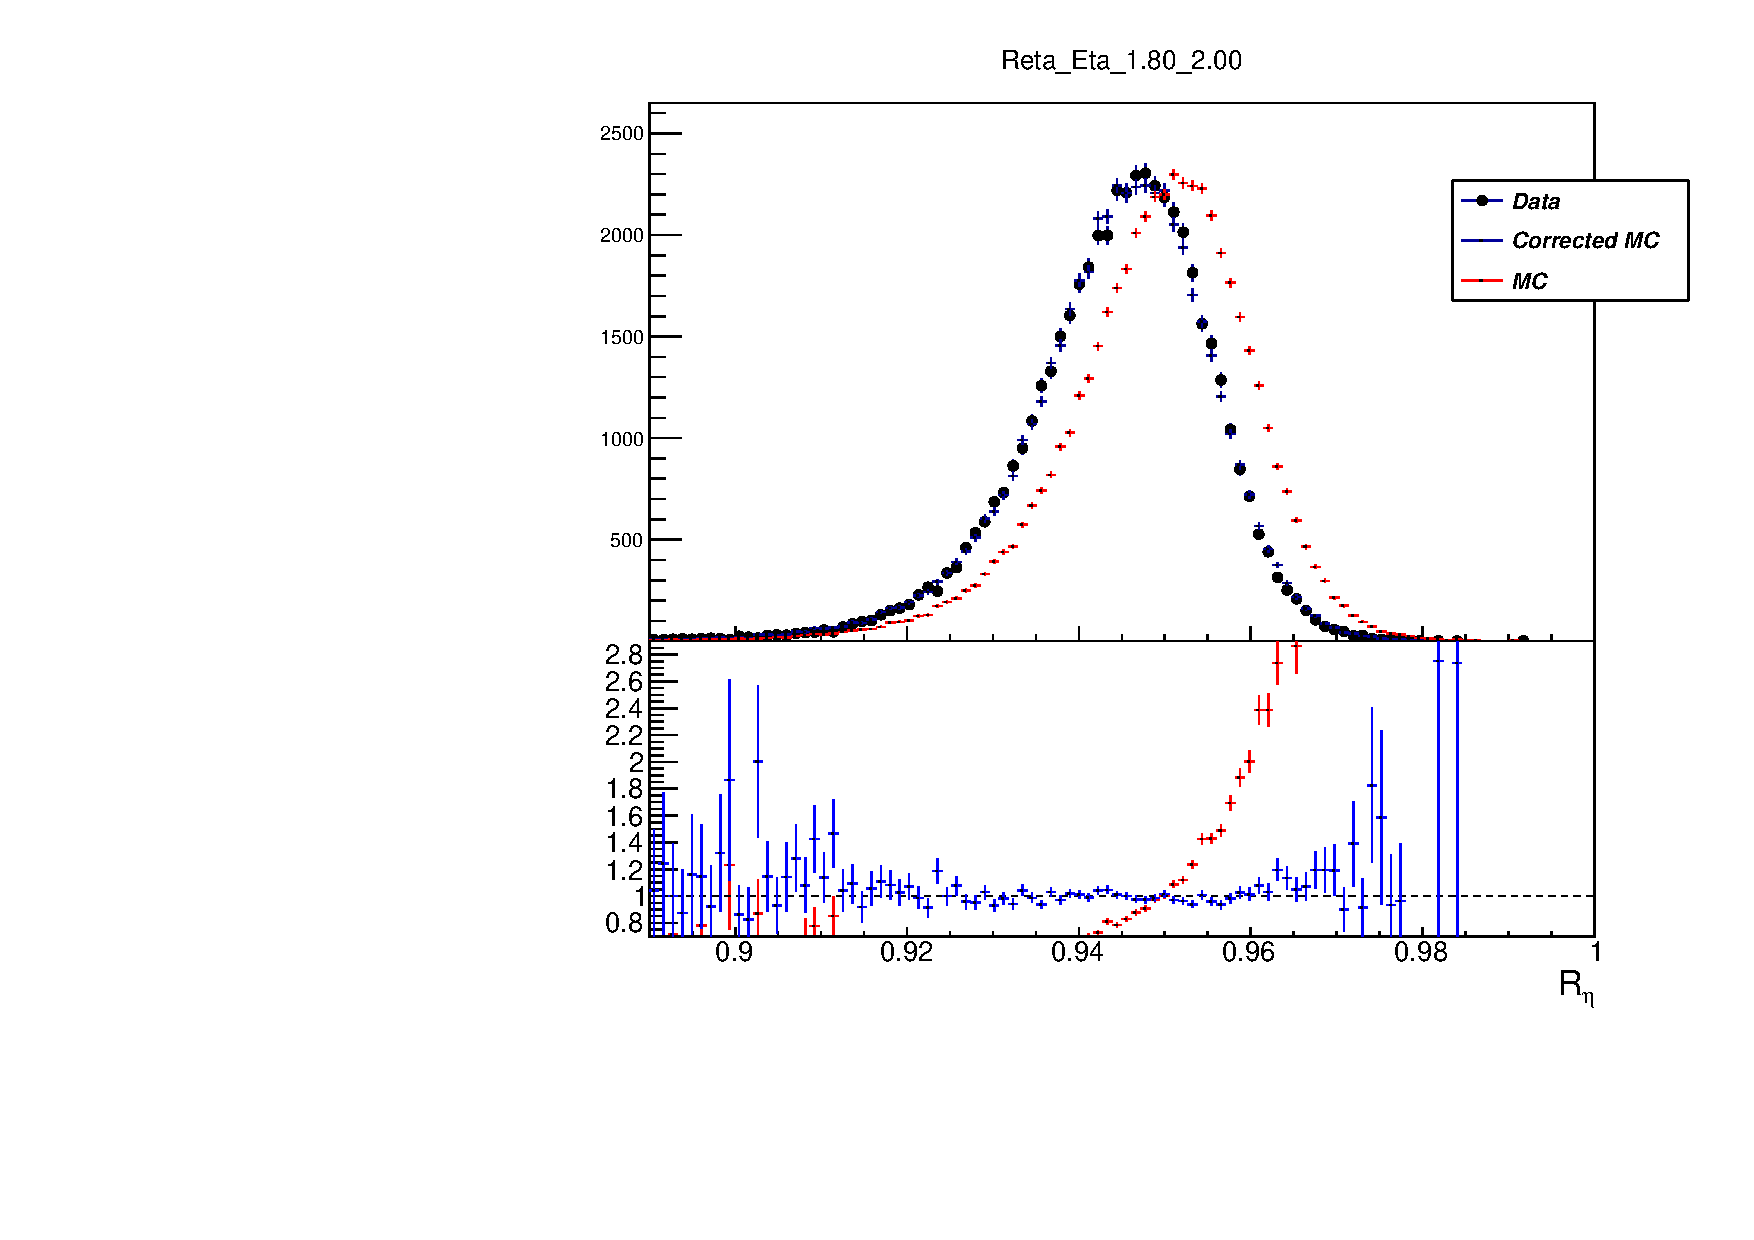
\includegraphics[width=\textwidth,keepaspectratio]{Reta_Eta_18_20_Athena.pdf}
  		\caption{Reweighted  $R_{\eta }$ in $|\eta| = (1.8,2.0)$.  }
  		\label{fig::pd}
  	\end{subfigure}
  	\caption{$R_{\eta }$  in the barrel and in the end-cap}
  	\label{fig::reta}
  \end{figure}
 
      \begin{figure}[htbp]
  	\begin{subfigure}[t]{0.5\textwidth}
  		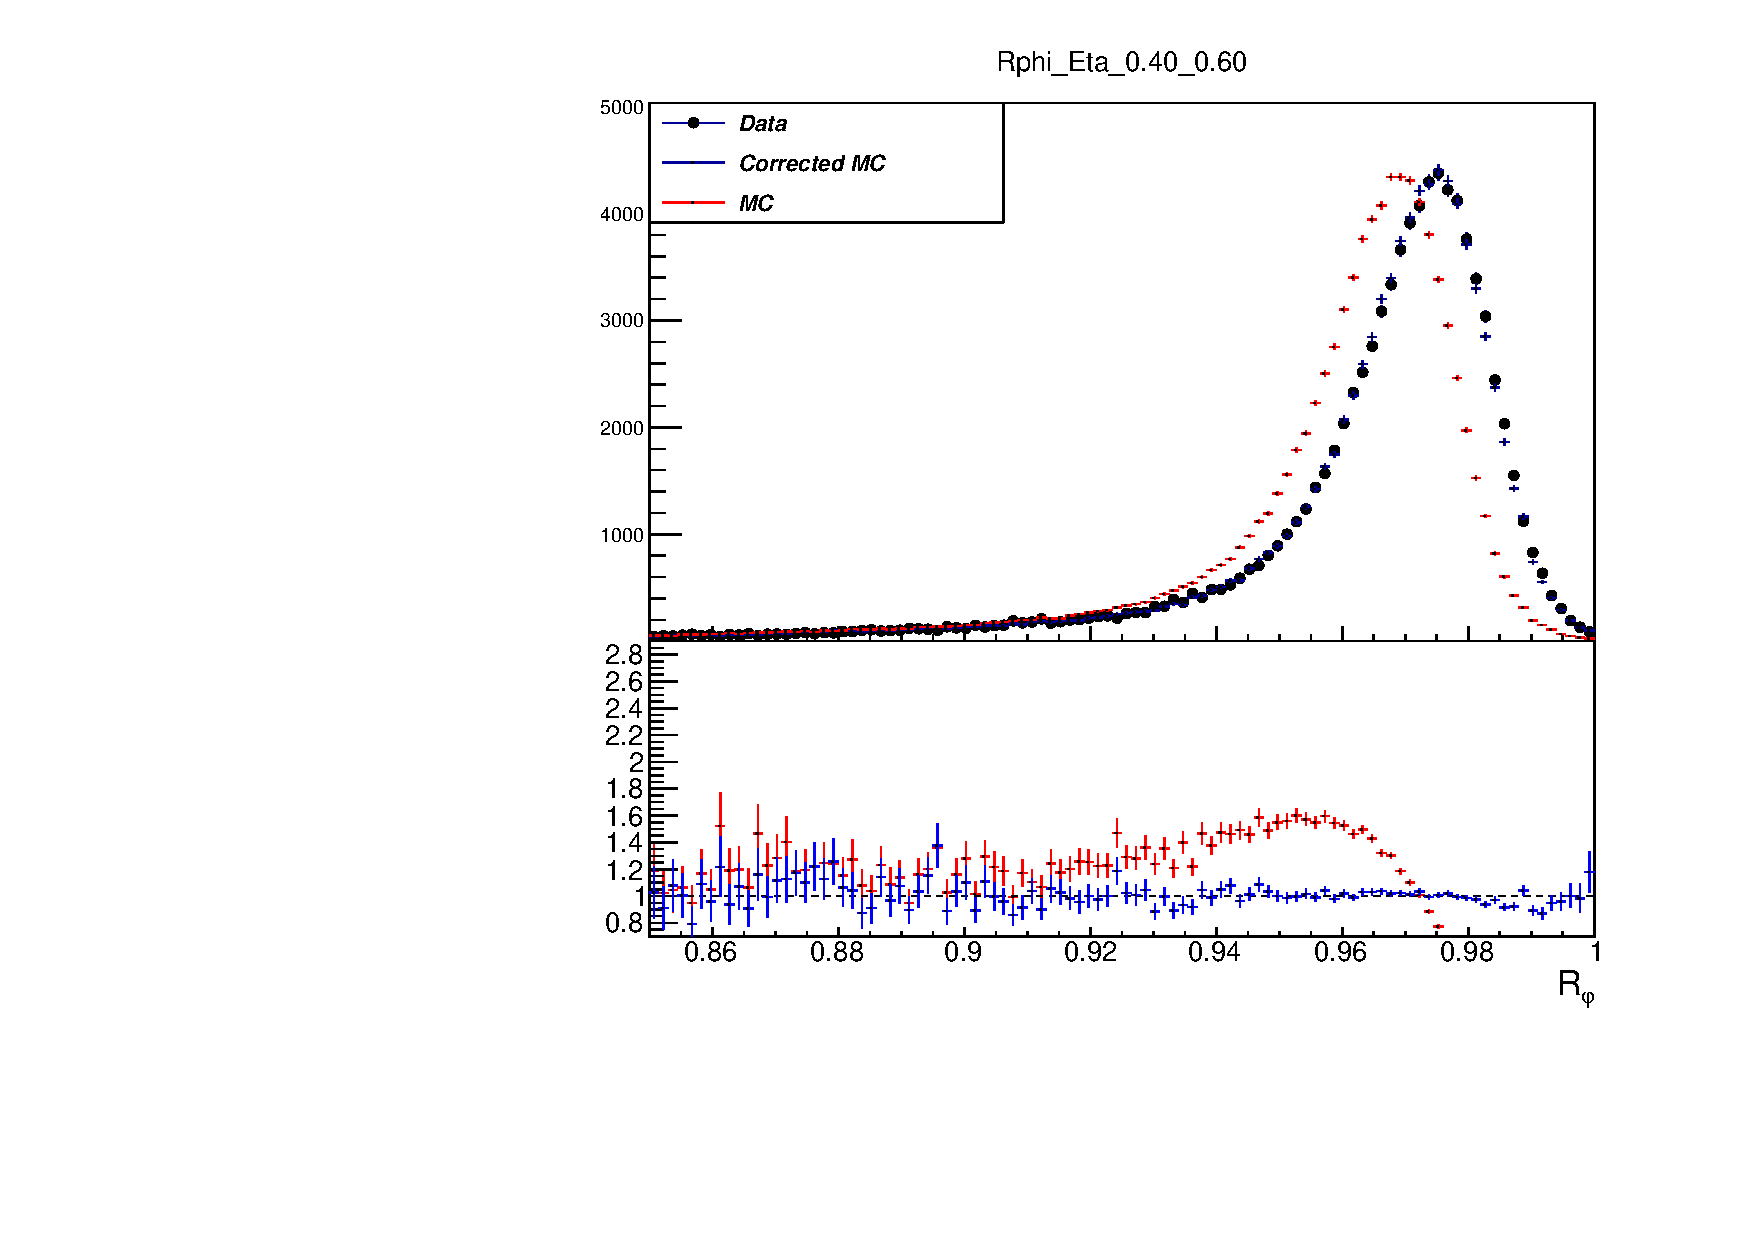
\includegraphics[width=\textwidth,keepaspectratio]{Rphi_Eta_4_6_Athena.pdf}
  		\caption{$R_{\phi}$ in $|\eta| = (0.4,0.6)$ }
  		\label{fig::rphi_rew_04}
  	\end{subfigure}
  	\hfill
  	\begin{subfigure}[t]{0.5\textwidth} 
  		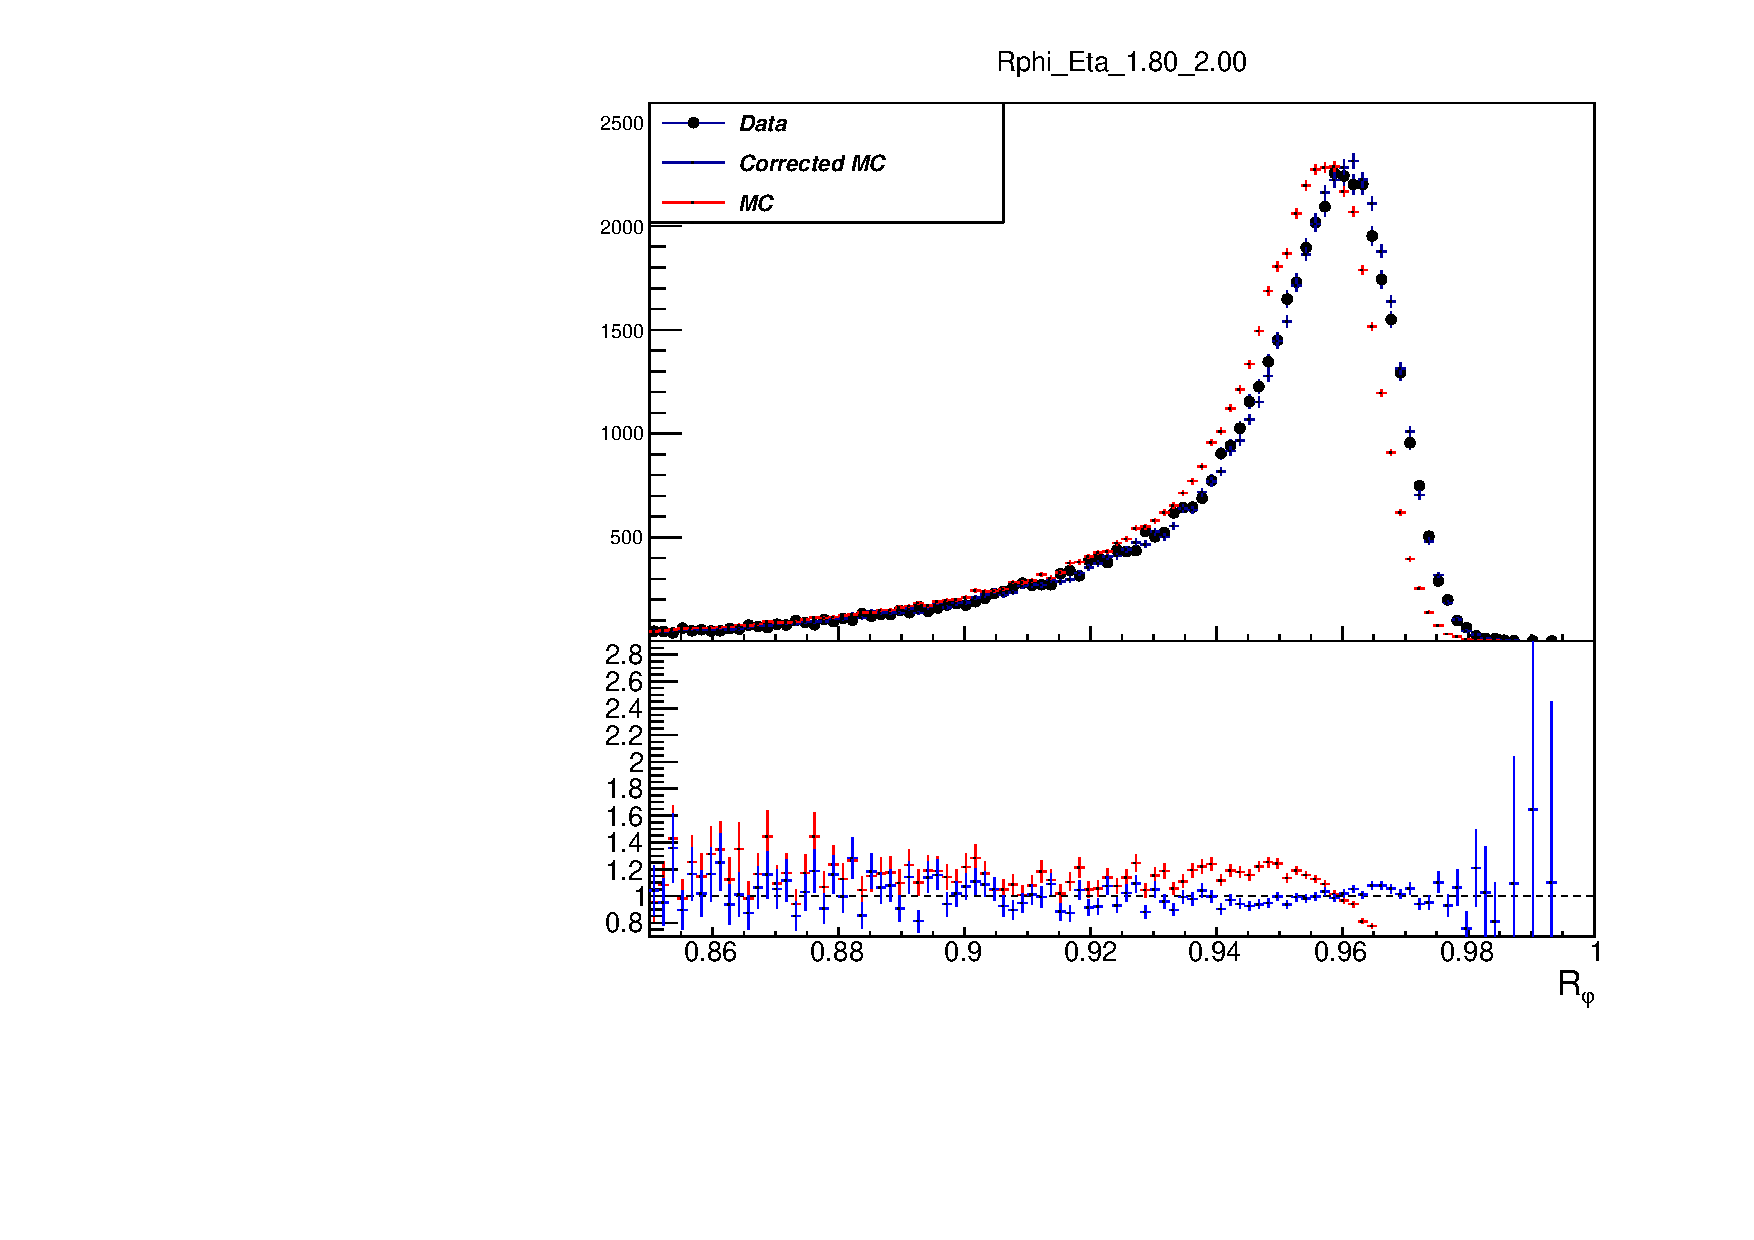
\includegraphics[width=\textwidth,keepaspectratio]{Rphi_Eta_18_20_Athena.pdf}
  		\caption{$R_{\phi}$ in $|\eta| = (1.8,2.0)$ }
  		\label{fig::rphi_rew_18}
  	\end{subfigure}
  	\caption{$R_{\phi}$ in the barel and in the end-cap, Data, MC, reweighted MC}
  	\label{fig::rphi_rew}
  \end{figure}
  
    \begin{figure}[htbp]
	\begin{subfigure}[t]{0.5\textwidth}
		\includegraphics[width=\textwidth,keepaspectratio]{weta2_Eta_4_6_Athena.pdf}
		\caption{$W_{\eta}^2$ in $|\eta| = (0.4,0.6)$ }
		\label{fig::weta2_rew_04}
	\end{subfigure}
	\hfill
	\begin{subfigure}[t]{0.5\textwidth} 
		\includegraphics[width=\textwidth,keepaspectratio]{weta2_Eta_18_20.pdf}
		\caption{$W_{\eta}^2$ in $|\eta| = (1.8,2.0)$ }
		\label{fig::weta2_rew_18}
	\end{subfigure}
	\caption{$W_{\eta}^2$ in the barel and in the end-cap, Data, MC, reweighted MC}
	\label{fig::weta2_rew}
\end{figure}

\begin{figure*}[ht!]
	\subfloat{%
		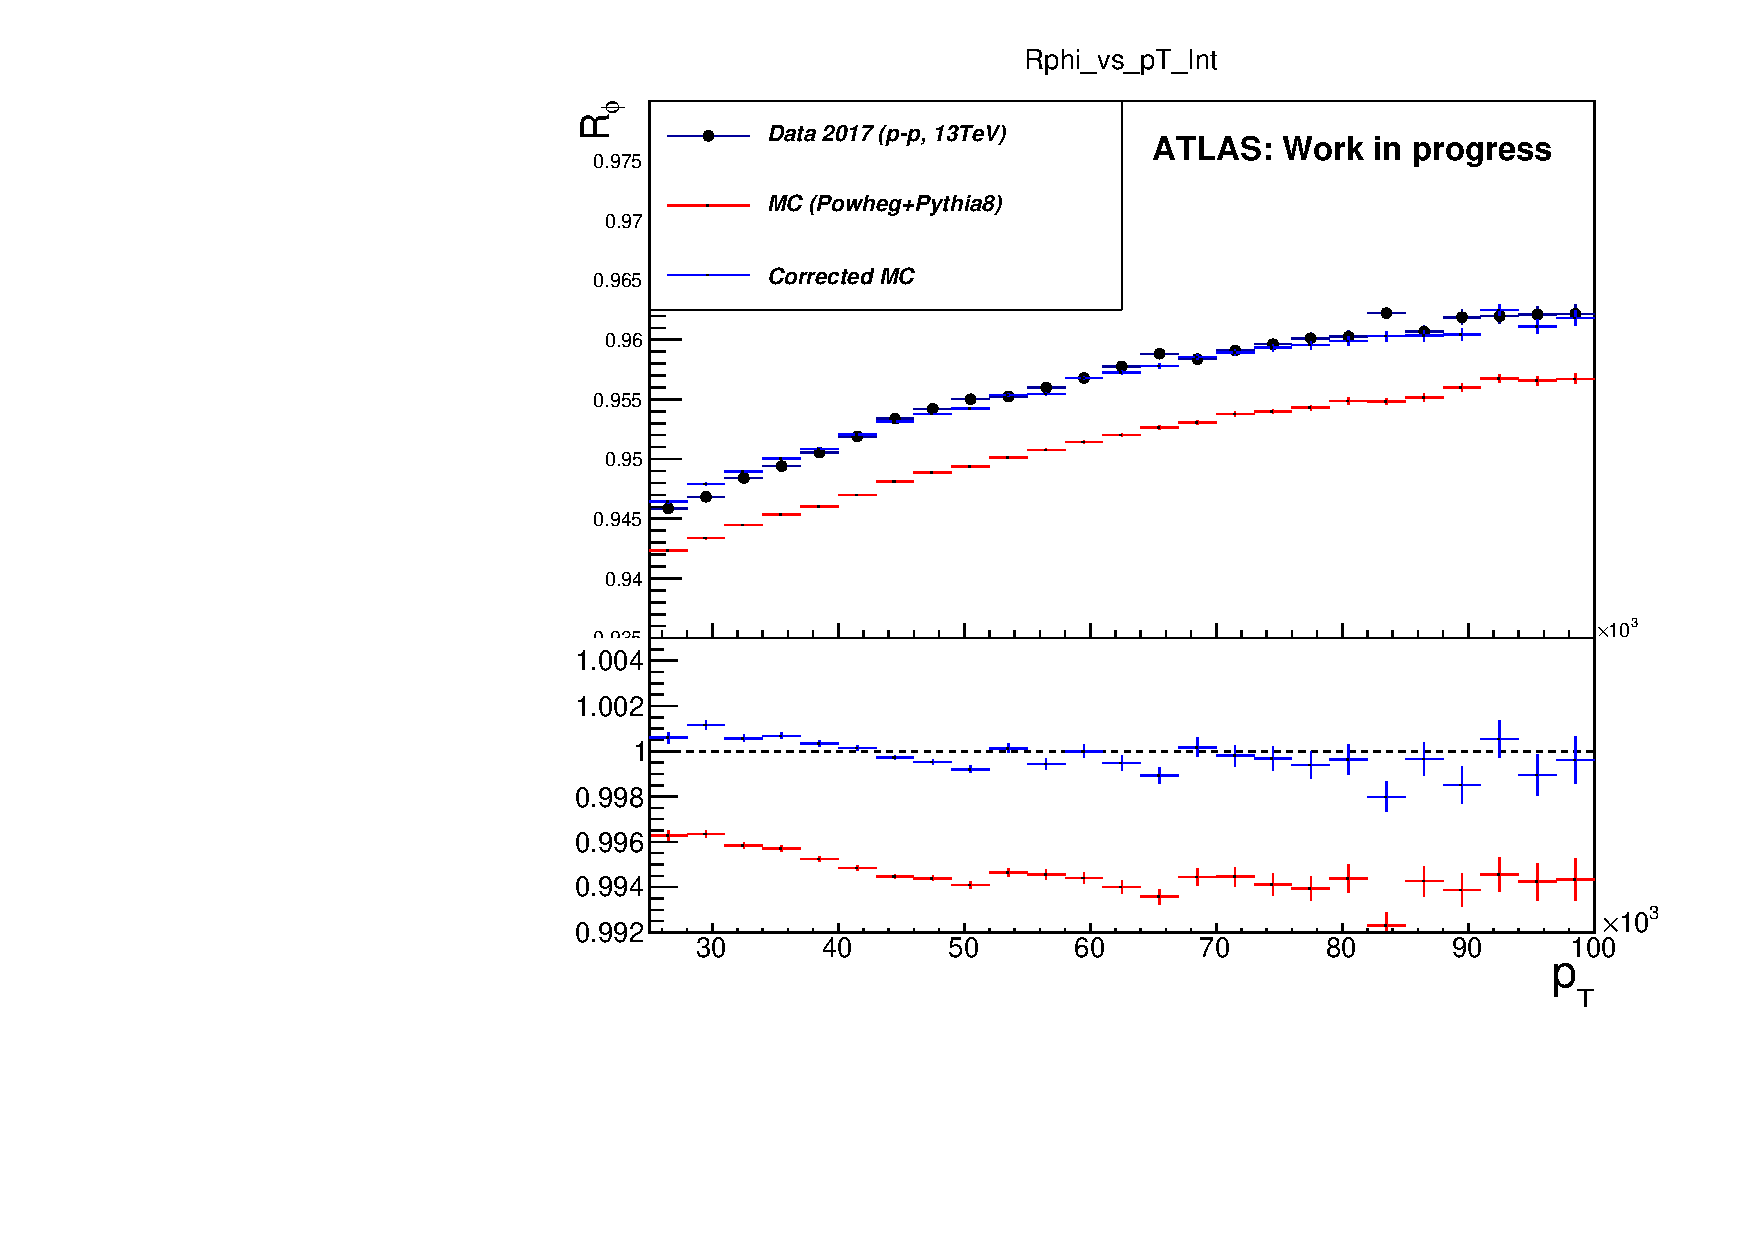
\includegraphics[width=0.33\textwidth]{Rphi_vs_pT_Int}}
	\quad
	\subfloat {%
		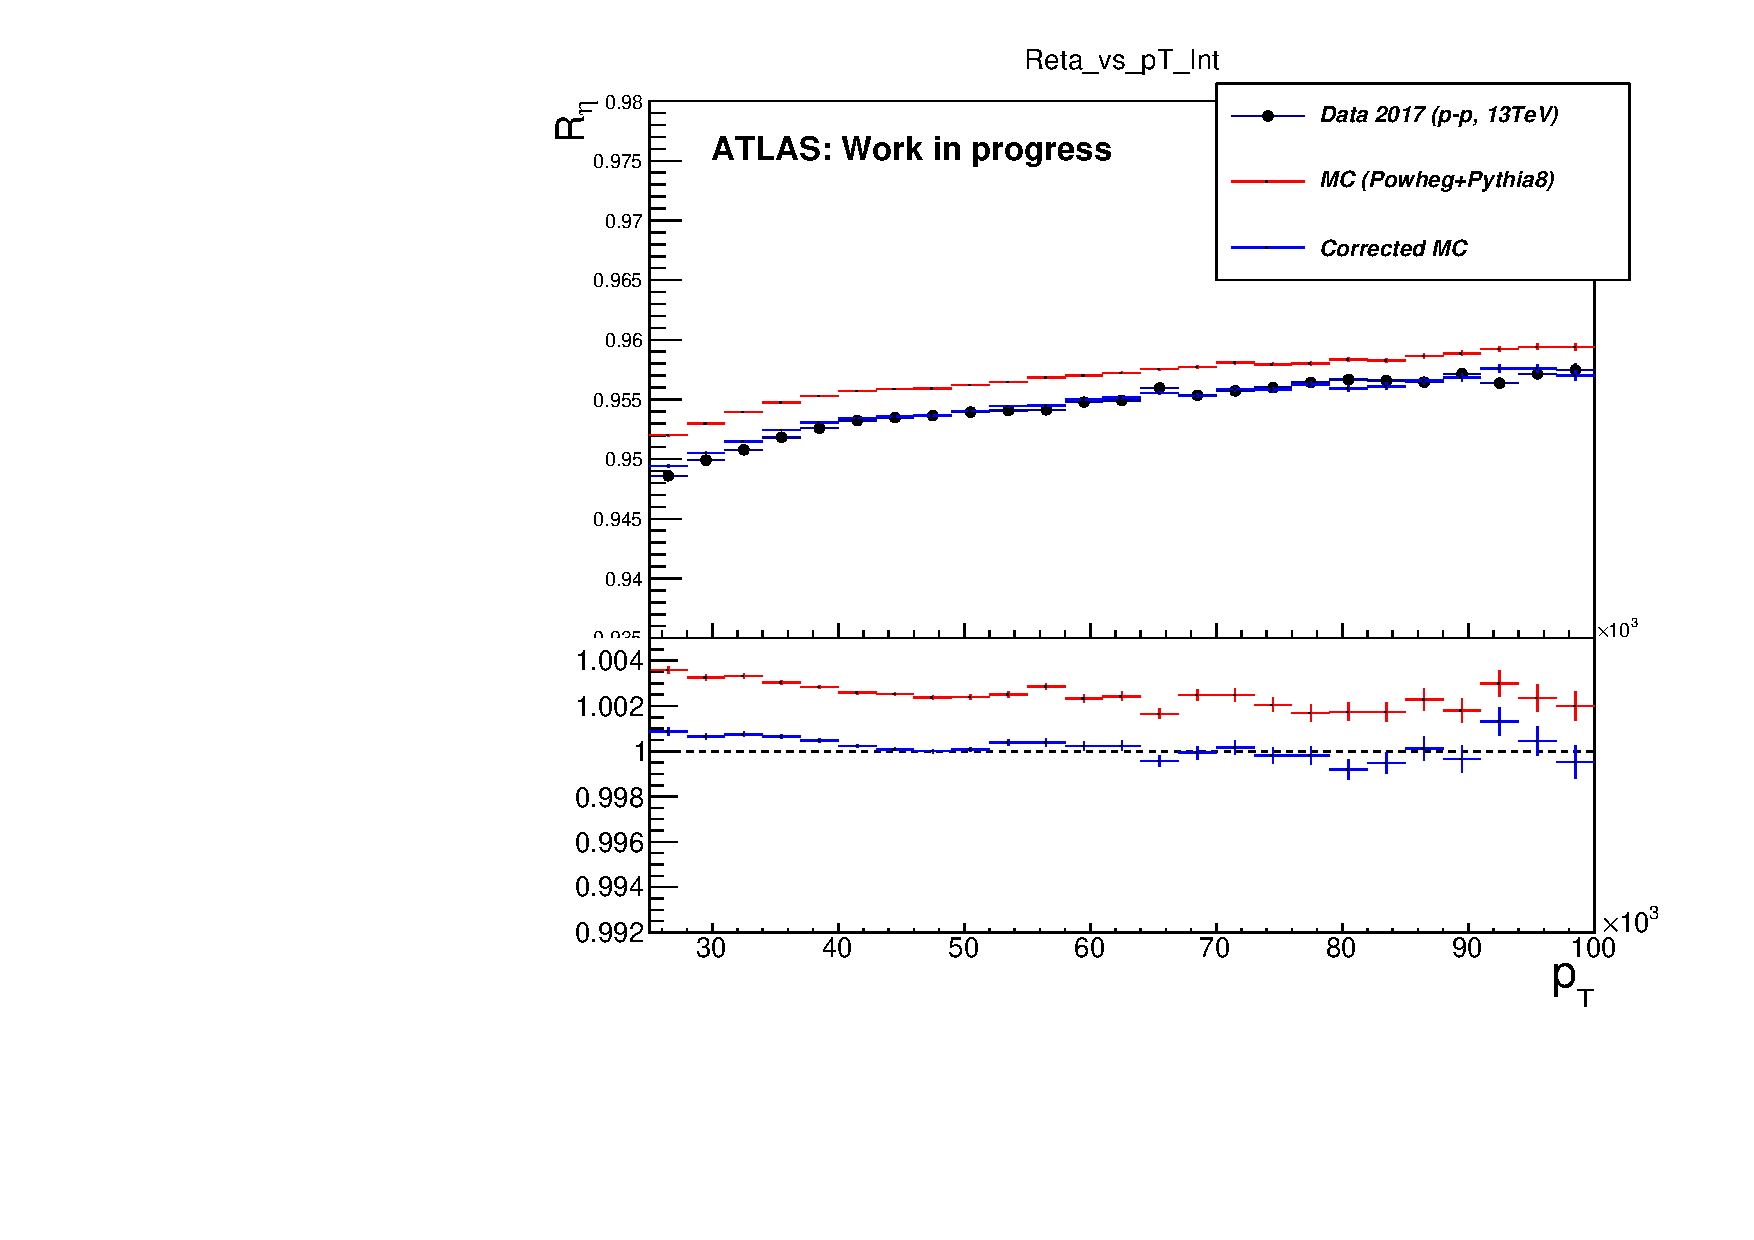
\includegraphics[width=0.33\textwidth]{Reta_vs_pT_Int}}
	\quad
	\subfloat{%
		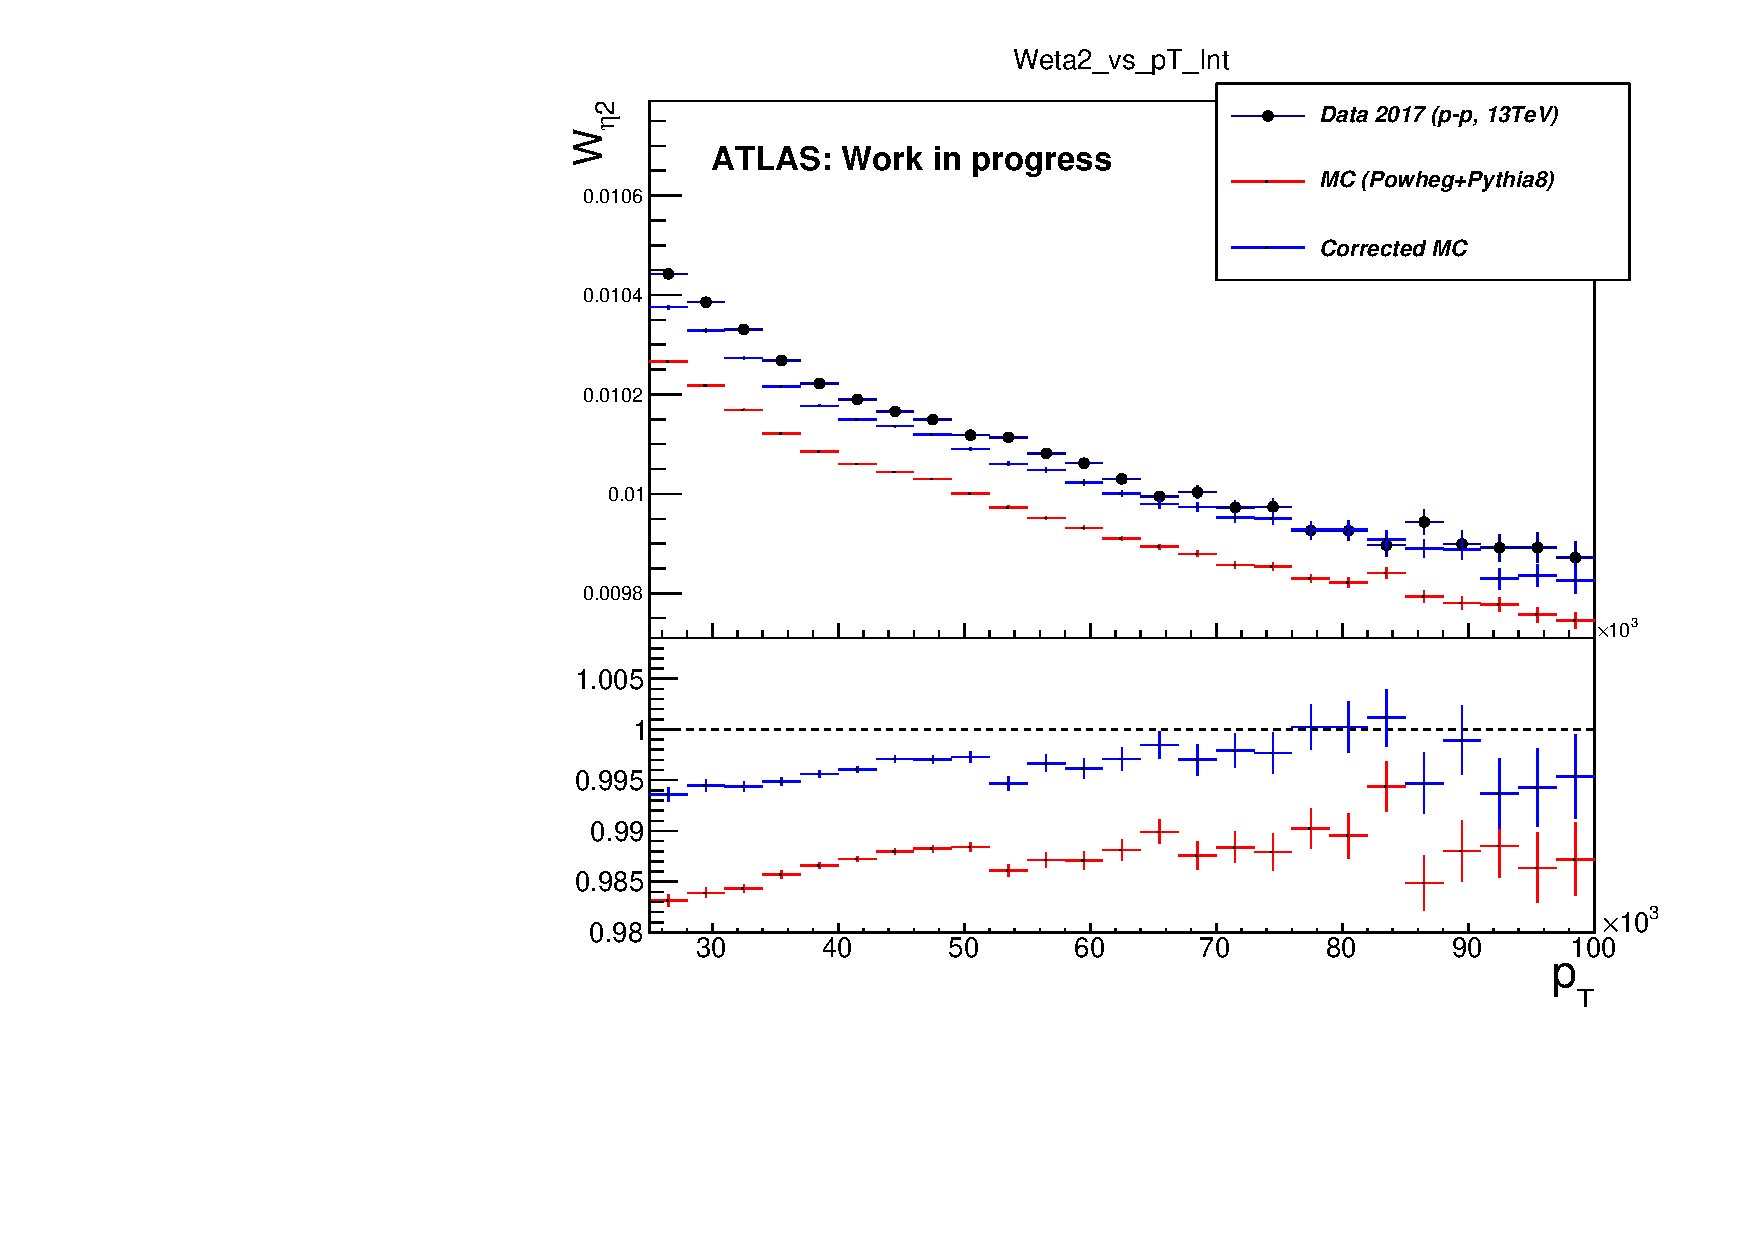
\includegraphics[width=0.33\textwidth]{Weta2_vs_pT_Int}}\\

	\caption{ 	\label{fig::integrated} Distributions integrated over pT (a) $R_{\phi}$; (b) $R_{\eta}$; (c)$W_{\eta 2}$.}
\end{figure*}


  
  \begin{figure}[htbp]
  	\centering
  	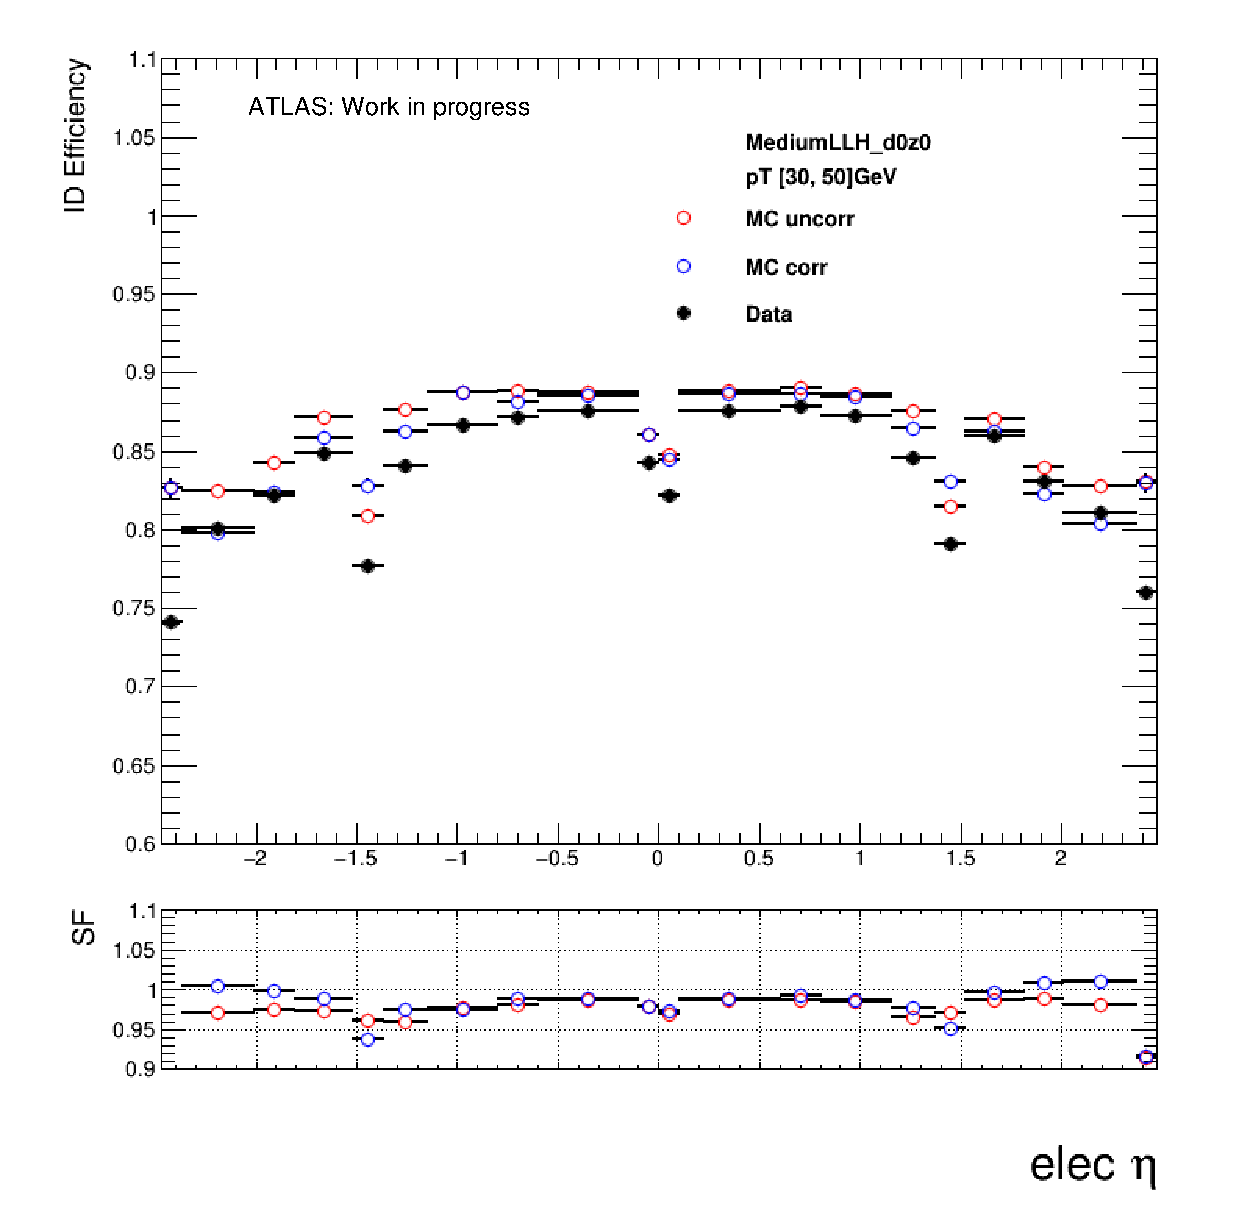
\includegraphics[width=7cm,keepaspectratio]{MCeffm247tom237.pdf}\\
  	\caption{Electron identification efficiency as a function of the electron pseudo-rapidity}
  	\label{SF}
  \end{figure}
  \section{Appendix: control plots}

  \begin{figure*}[ht!]
  	\subfloat{%
  		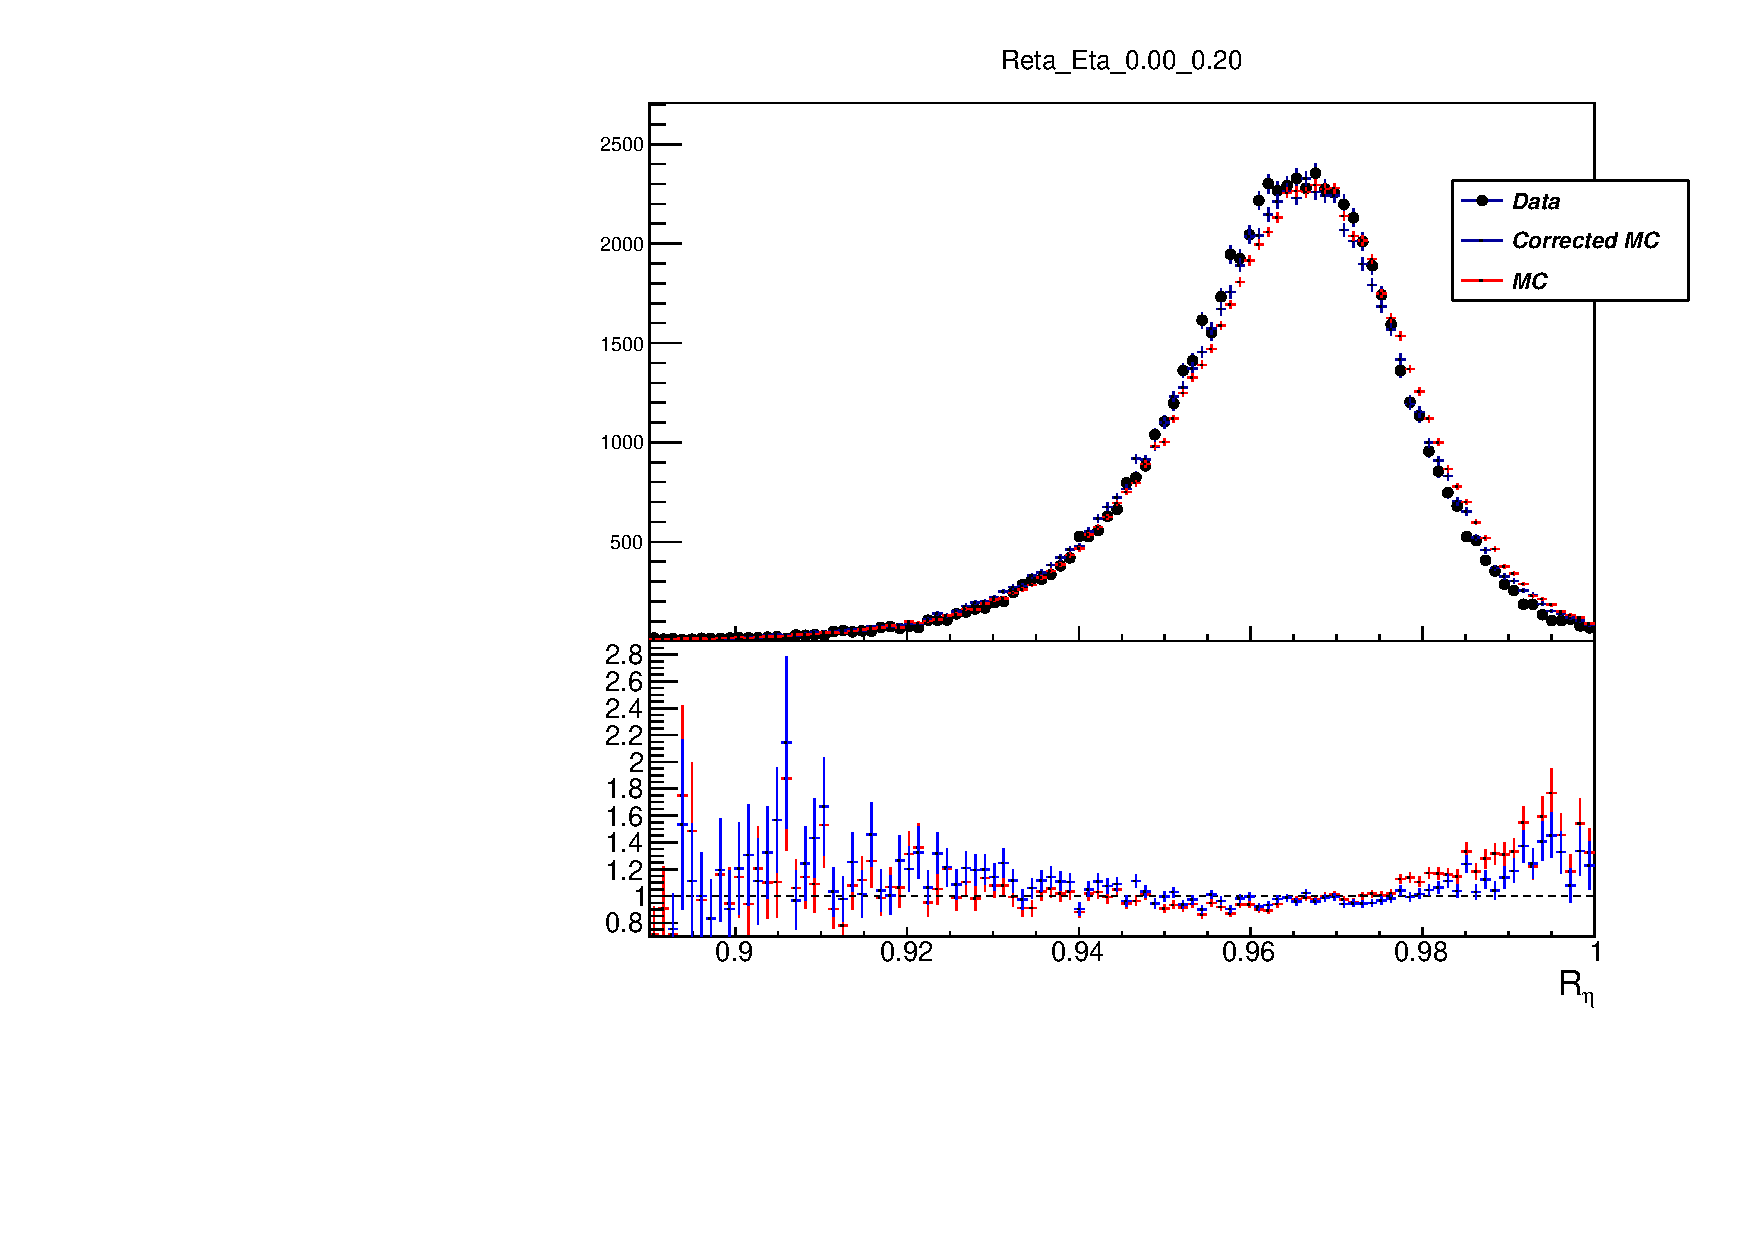
\includegraphics[width=0.33\textwidth]{Reta_Eta_0_2_Athena}}
  	\quad
  	\subfloat {%
  		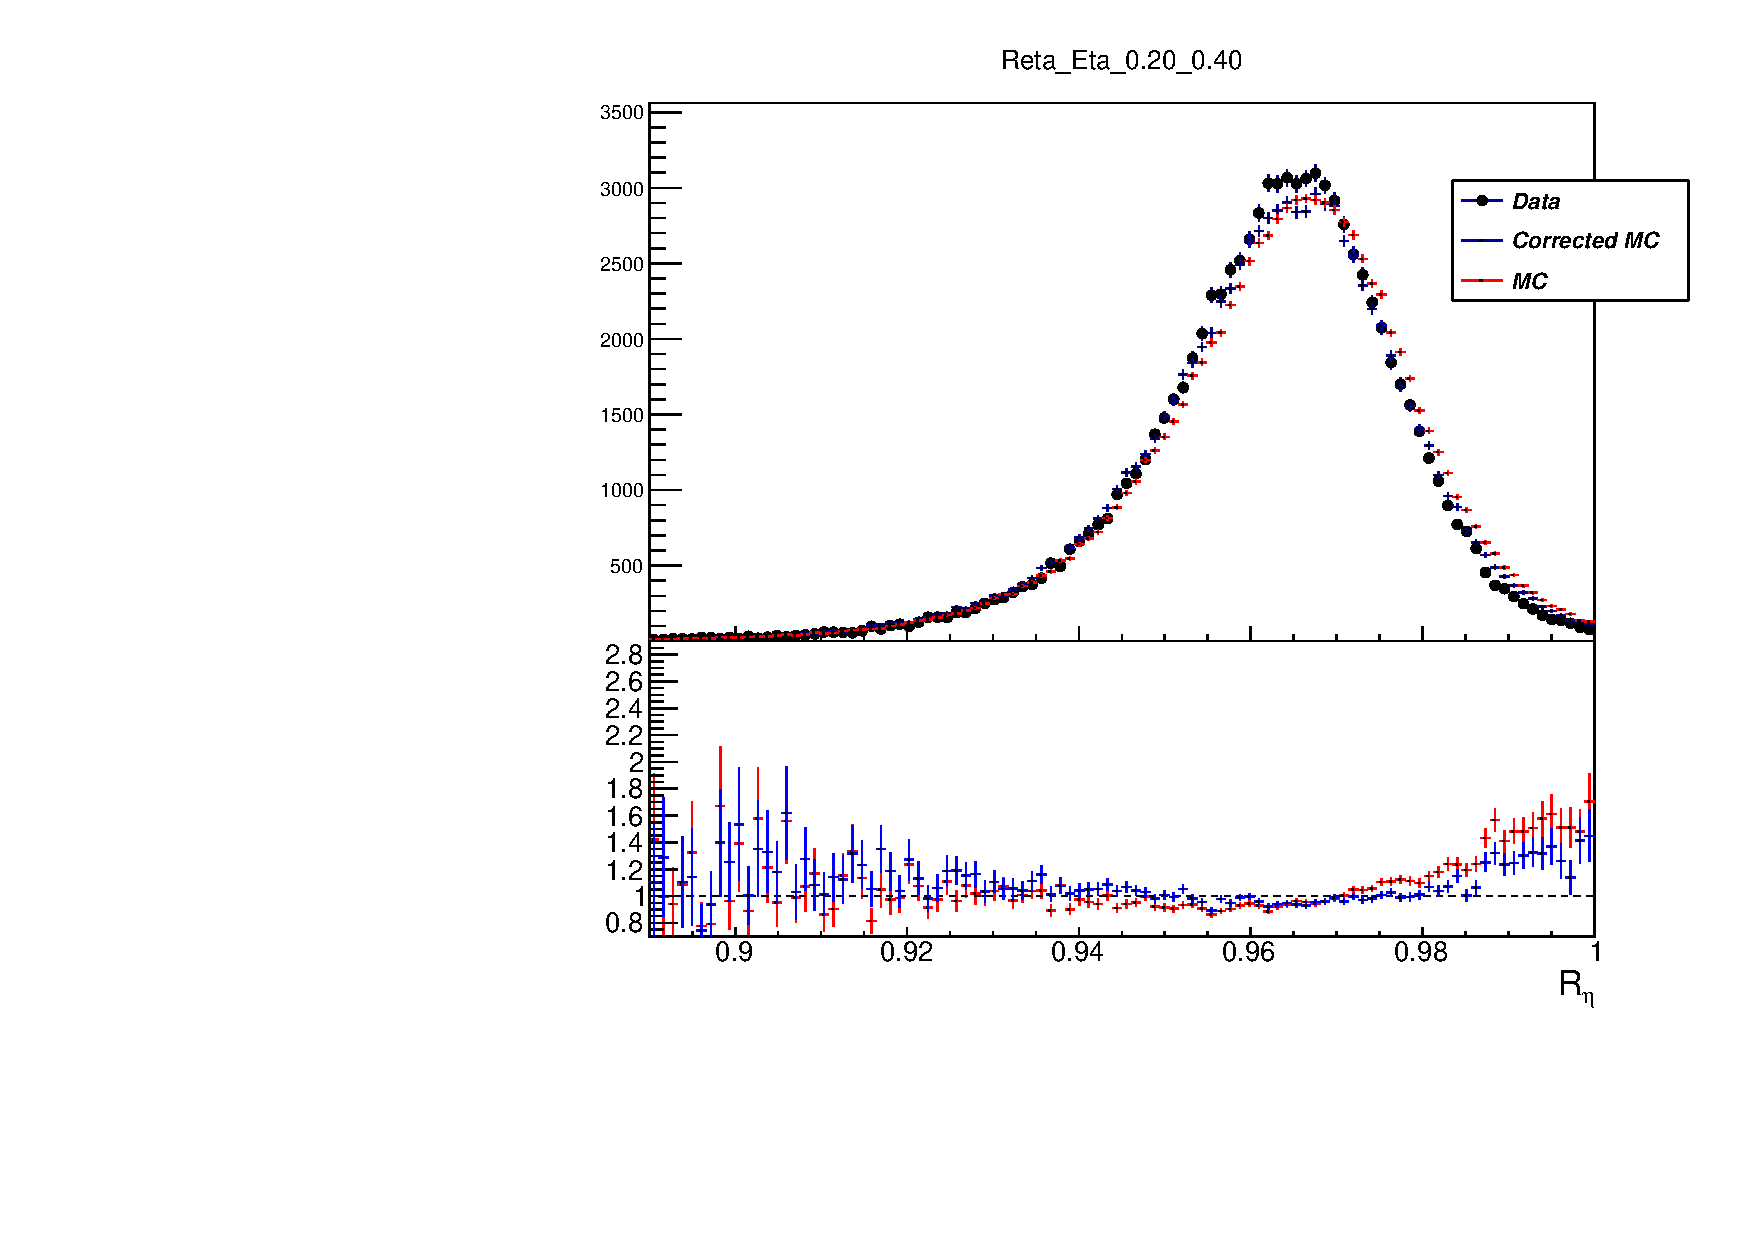
\includegraphics[width=0.33\textwidth]{Reta_Eta_2_4_Athena}}
  	\quad
  	\subfloat{%
  		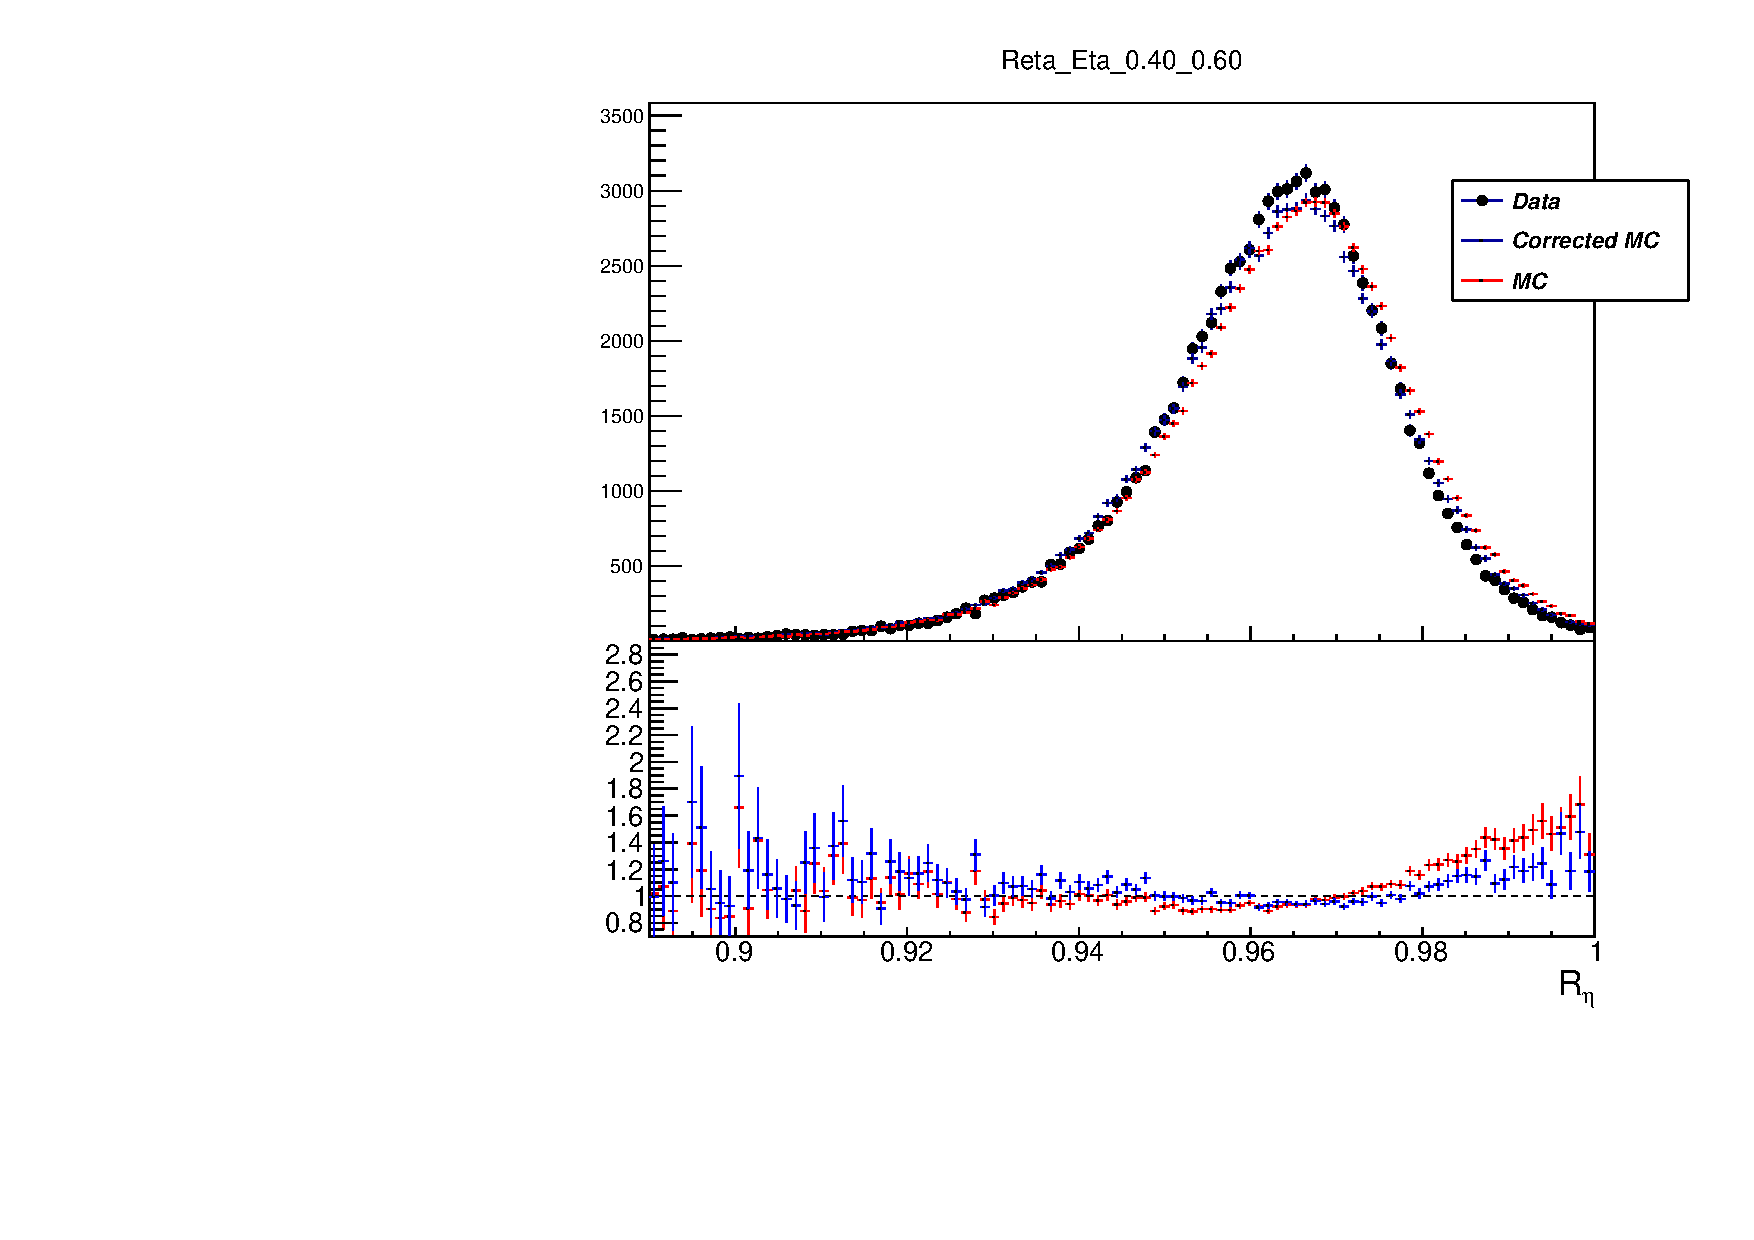
\includegraphics[width=0.33\textwidth]{Reta_Eta_4_6_Athena}}\\
  	\subfloat{%
  		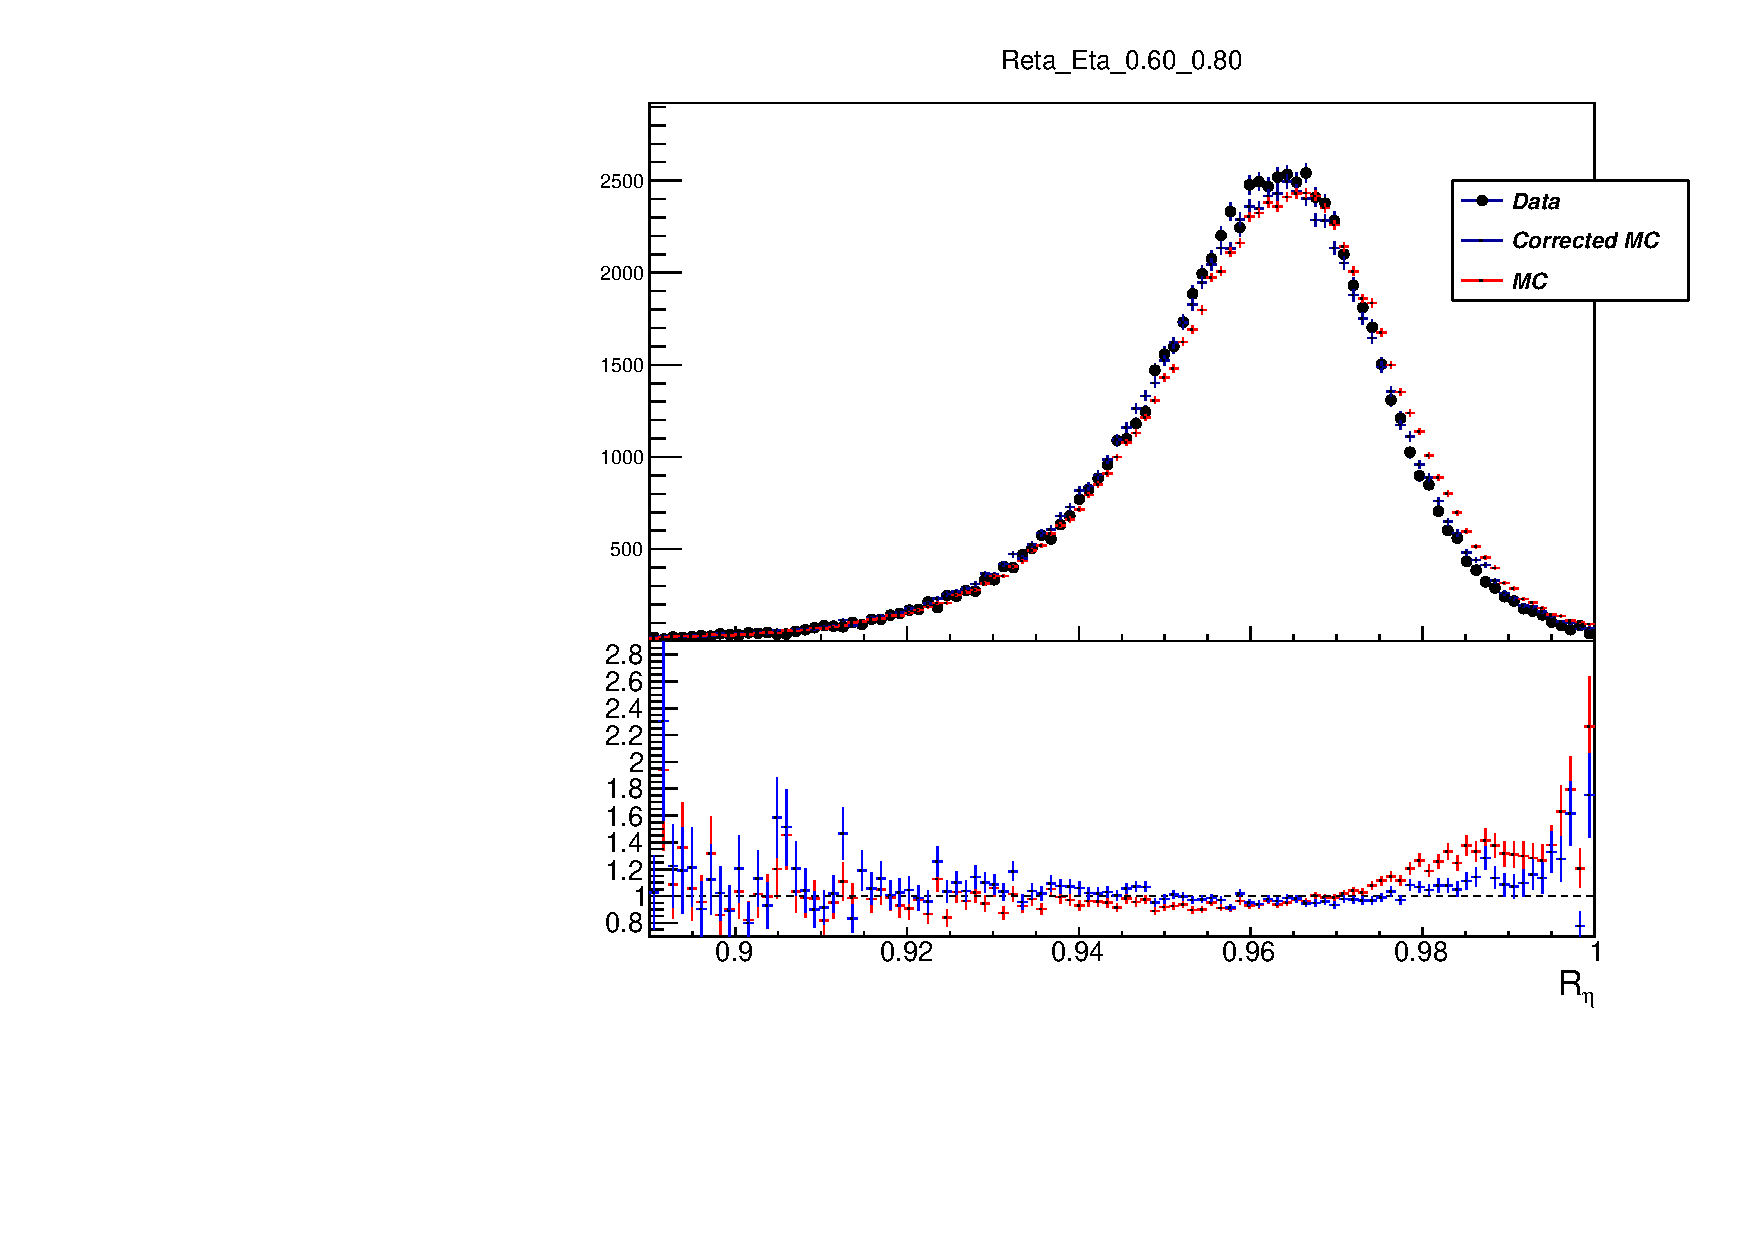
\includegraphics[width=0.33\textwidth]{Reta_Eta_6_8_Athena}}
  	\quad
  	\subfloat {%
  		\includegraphics[width=0.33\textwidth]{Reta_Eta_8_10_Athena}}
  	\quad
  	\subfloat{%
  		\includegraphics[width=0.33\textwidth]{Reta_Eta_10_12_Athena}}\\
	\subfloat{%
		\includegraphics[width=0.33\textwidth]{Reta_Eta_12_13_Athena}}
	\quad
	\subfloat{%
		\includegraphics[width=0.33\textwidth]{Reta_Eta_152_16_Athena}}
	\subfloat{%
			\includegraphics[width=0.33\textwidth]{Reta_Eta_16_18_Athena}}\\
	\quad
	\subfloat {%
		\includegraphics[width=0.33\textwidth]{Reta_Eta_16_18_Athena}}
	\quad
	\subfloat{%
		\includegraphics[width=0.33\textwidth]{Reta_Eta_20_22_Athena}}
		\quad
	\subfloat{%
		\includegraphics[width=0.33\textwidth]{Reta_Eta_22_24_Athena}}
	\caption{ 	\label{fig::reta_} Reta 2}
\end{figure*}

  \begin{figure*}[ht!]
	\subfloat{%
		\includegraphics[width=0.33\textwidth]{Rphi_Eta_0_2_Athena}}
	\quad
	\subfloat {%
		\includegraphics[width=0.33\textwidth]{Rphi_Eta_2_4_Athena}}
	\quad
	\subfloat{%
		\includegraphics[width=0.33\textwidth]{Rphi_Eta_4_6_Athena}}\\
	\subfloat{%
		\includegraphics[width=0.33\textwidth]{Rphi_Eta_6_8_Athena}}
	\quad
	\subfloat {%
		\includegraphics[width=0.33\textwidth]{Rphi_Eta_8_10_Athena}}
	\quad
	\subfloat{%
		\includegraphics[width=0.33\textwidth]{Rphi_Eta_10_12_Athena}}\\
	\subfloat{%
		\includegraphics[width=0.33\textwidth]{Rphi_Eta_12_13_Athena}}
	\quad
	\subfloat{%
		\includegraphics[width=0.33\textwidth]{Rphi_Eta_152_16_Athena}}
	\subfloat{%
		\includegraphics[width=0.33\textwidth]{Rphi_Eta_16_18_Athena}}\\
	\quad
	\subfloat {%
		\includegraphics[width=0.33\textwidth]{Rphi_Eta_16_18_Athena}}
	\quad
	\subfloat{%
		\includegraphics[width=0.33\textwidth]{Rphi_Eta_20_22_Athena}}
	\quad
	\subfloat{%
		\includegraphics[width=0.33\textwidth]{Rphi_Eta_22_24_Athena}}
	\caption{ 	\label{fig::rphi_} Rphi in all eta slices}
\end{figure*}

  \begin{figure*}[ht!]
	\subfloat{%
		\includegraphics[width=0.33\textwidth]{Weta2_Eta_0_2_Athena}}
	\quad
	\subfloat {%
		\includegraphics[width=0.33\textwidth]{Weta2_Eta_2_4_Athena}}
	\quad
	\subfloat{%
		\includegraphics[width=0.33\textwidth]{Weta2_Eta_4_6_Athena}}\\
	\subfloat{%
		\includegraphics[width=0.33\textwidth]{Weta2_Eta_6_8_Athena}}
	\quad
	\subfloat {%
		\includegraphics[width=0.33\textwidth]{Weta2_Eta_8_10_Athena}}
	\quad
	\subfloat{%
		\includegraphics[width=0.33\textwidth]{Weta2_Eta_10_12_Athena}}\\
	\subfloat{%
		\includegraphics[width=0.33\textwidth]{Weta2_Eta_12_13_Athena}}
	\quad
	\subfloat{%
		\includegraphics[width=0.33\textwidth]{Weta2_Eta_152_16_Athena}}
	\subfloat{%
		\includegraphics[width=0.33\textwidth]{Weta2_Eta_16_18_Athena}}\\
	\quad
	\subfloat {%
		\includegraphics[width=0.33\textwidth]{Weta2_Eta_16_18_Athena}}
	\quad
	\subfloat{%
		\includegraphics[width=0.33\textwidth]{Weta2_Eta_20_22_Athena}}
	\quad
	\subfloat{%
		\includegraphics[width=0.33\textwidth]{Weta2_Eta_22_24_Athena}}
	\caption{ 	\label{fig::weta2_} Reta 2}
\end{figure*}

  \begin{figure*}[ht!]
	\subfloat{%
		\includegraphics[width=0.33\textwidth]{Weta2_Eta_0_2_Athena}}
	\quad
	\subfloat {%
		\includegraphics[width=0.33\textwidth]{Weta2_Eta_2_4_Athena}}
	\quad
	\subfloat{%
		\includegraphics[width=0.33\textwidth]{Weta2_Eta_4_6_Athena}}\\
	\subfloat{%
		\includegraphics[width=0.33\textwidth]{Weta2_Eta_6_8_Athena}}
	\quad
	\subfloat {%
		\includegraphics[width=0.33\textwidth]{Weta2_Eta_8_10_Athena}}
	\quad
	\subfloat{%
		\includegraphics[width=0.33\textwidth]{Weta2_Eta_10_12_Athena}}\\
	\subfloat{%
		\includegraphics[width=0.33\textwidth]{Weta2_Eta_12_13_Athena}}
	\quad
	\subfloat{%
		\includegraphics[width=0.33\textwidth]{Weta2_Eta_152_16_Athena}}
	\subfloat{%
		\includegraphics[width=0.33\textwidth]{Weta2_Eta_16_18_Athena}}\\
	\quad
	\subfloat {%
		\includegraphics[width=0.33\textwidth]{Weta2_Eta_16_18_Athena}}
	\quad
	\subfloat{%
		\includegraphics[width=0.33\textwidth]{Weta2_Eta_20_22_Athena}}
	\quad
	\subfloat{%
		\includegraphics[width=0.33\textwidth]{Weta2_Eta_22_24_Athena}}
	\caption{ 	\label{fig::weta2_} Reta 2}
\end{figure*}

  \begin{figure*}[ht!]
	\subfloat{%
		\includegraphics[width=0.33\textwidth]{etaProfile_Eta_0_2_Athena}}
	\quad
	\subfloat {%
		\includegraphics[width=0.33\textwidth]{etaProfile_Eta_2_4_Athena}}
	\quad
	\subfloat{%
		\includegraphics[width=0.33\textwidth]{etaProfile_Eta_4_6_Athena}}\\
	\subfloat{%
		\includegraphics[width=0.33\textwidth]{etaProfile_Eta_6_8_Athena}}
	\quad
	\subfloat {%
		\includegraphics[width=0.33\textwidth]{etaProfile_Eta_8_10_Athena}}
	\quad
	\subfloat{%
		\includegraphics[width=0.33\textwidth]{etaProfile_Eta_10_12_Athena}}\\
	\subfloat{%
		\includegraphics[width=0.33\textwidth]{etaProfile_Eta_12_13_Athena}}
	\quad
	\subfloat{%
		\includegraphics[width=0.33\textwidth]{etaProfile_Eta_152_16_Athena}}
	\subfloat{%
		\includegraphics[width=0.33\textwidth]{etaProfile_Eta_16_18_Athena}}\\
	\quad
	\subfloat {%
		\includegraphics[width=0.33\textwidth]{etaProfile_Eta_16_18_Athena}}
	\quad
	\subfloat{%
		\includegraphics[width=0.33\textwidth]{etaProfile_Eta_20_22_Athena}}
	\quad
	\subfloat{%
		\includegraphics[width=0.33\textwidth]{etaProfile_Eta_22_24_Athena}}
	\caption{ 	\label{fig::etaProfile_} Reta 2}
\end{figure*}


  \begin{figure*}[ht!]
	\subfloat{%
		\includegraphics[width=0.33\textwidth]{phiProfile_Eta_0_2_Athena}}
	\quad
	\subfloat {%
		\includegraphics[width=0.33\textwidth]{phiProfile_Eta_2_4_Athena}}
	\quad
	\subfloat{%
		\includegraphics[width=0.33\textwidth]{phiProfile_Eta_4_6_Athena}}\\
	\subfloat{%
		\includegraphics[width=0.33\textwidth]{phiProfile_Eta_6_8_Athena}}
	\quad
	\subfloat {%
		\includegraphics[width=0.33\textwidth]{phiProfile_Eta_8_10_Athena}}
	\quad
	\subfloat{%
		\includegraphics[width=0.33\textwidth]{phiProfile_Eta_10_12_Athena}}\\
	\subfloat{%
		\includegraphics[width=0.33\textwidth]{phiProfile_Eta_12_13_Athena}}
	\quad
	\subfloat{%
		\includegraphics[width=0.33\textwidth]{phiProfile_Eta_152_16_Athena}}
	\subfloat{%
		\includegraphics[width=0.33\textwidth]{phiProfile_Eta_16_18_Athena}}\\
	\quad
	\subfloat {%
		\includegraphics[width=0.33\textwidth]{phiProfile_Eta_16_18_Athena}}
	\quad
	\subfloat{%
		\includegraphics[width=0.33\textwidth]{phiProfile_Eta_20_22_Athena}}
	\quad
	\subfloat{%
		\includegraphics[width=0.33\textwidth]{phiProfile_Eta_22_24_Athena}}
	\caption{ 	\label{fig::phiProfile_} Reta 2}
\end{figure*}

  \begin{figure*}[ht!]
	\subfloat{%
		\includegraphics[width=0.33\textwidth]{wtots1_Eta_0_2}}
	\quad
	\subfloat {%
		\includegraphics[width=0.33\textwidth]{wtots1_Eta_2_4}}
	\quad
	\subfloat{%
		\includegraphics[width=0.33\textwidth]{wtots1_Eta_4_6}}\\
	\subfloat{%
		\includegraphics[width=0.33\textwidth]{wtots1_Eta_6_8}}
	\quad
	\subfloat {%
		\includegraphics[width=0.33\textwidth]{wtots1_Eta_8_10}}
	\quad
	\subfloat{%
		\includegraphics[width=0.33\textwidth]{wtots1_Eta_10_12}}\\
	\subfloat{%
		\includegraphics[width=0.33\textwidth]{wtots1_Eta_12_13}}
	\quad
	\subfloat{%
		\includegraphics[width=0.33\textwidth]{wtots1_Eta_13_137}}
	\subfloat{%
		\includegraphics[width=0.33\textwidth]{wtots1_Eta_16_18}}\\
	\quad
	\subfloat {%
		\includegraphics[width=0.33\textwidth]{wtots1_Eta_16_18}}
	\quad
	\subfloat{%
		\includegraphics[width=0.33\textwidth]{wtots1_Eta_20_22}}
	\quad
	\subfloat{%
		\includegraphics[width=0.33\textwidth]{wtots1_Eta_22_24}}
	\caption{ 	\label{fig::wtots1_} Reta 2}
\end{figure*}
%\newpage
%\chapter{Electromagnetic shower shapes correction }
	\label{ch::sshapes}
	The chapter considers the electromagnetic shower development in the ATLAS \gls{emc} and its role in particle identification (ID). The existing mismodelling of the shower development in the Monte-Carlo simulation causes discrepancies in electron ID. A correction method that allows to achieve good correspondence between the data and the simulation is proposed, implemented and tested.
  \section{Introduction}
  The design and functionality of the ATLAS electromagnetic calorimeter was described in \ref{emc}. Let's consider a bit more in detail the physical processes happening in the \gls{emc}. 
  
  It order to measure particle's energy within the calorimeter we must make the particle to loose its entire energy within the calorimeter. For the electrons and photons with energies over few MeV (which is the case for the ATLAS experiment) the primary energy loss mechanism lies in bremsstrahlung radiation and pair creation. The two processes complete each other, so when a high-energy electron or photon gets into the calorimeter, it creates an avalanche-like process called the electromagnetic shower when a bremsstrahlung-radiated photons create more electron-positron pairs which in turn radiate more bremsstrahlung photons and so on and so forth (see Fig. \ref{fig::em_shower}.)\\
  	\begin{figure}[htbp]
  	\begin{subfigure}[t]{0.5\textwidth}
  		\includegraphics[width=\textwidth,keepaspectratio]{em_shower.png}
  		\caption[Started by an electron]{Initiated by an electron}
  		\label{fig::id}
  	\end{subfigure}
  	\hfill
  	\begin{subfigure}[t]{0.5\textwidth} 
  		\includegraphics[width=\textwidth,keepaspectratio]{emshower.png}
  		\caption[Started by a $\gamma$-photon]{Initiated by a $\gamma$-photon}
  		\label{fig::pd}
  	\end{subfigure}
  	\caption{The schematic portrayal of EM shower development}
  	\label{fig::em_shower}
  \end{figure}
    The longitudinal and transverse development of the shower depends on the type of the initial particle and on its energy. The energy is well measured by the calorimeter, but identifying the particle still remains a challenging task. The transverse granularity of the ATLAS calorimeter allows to resolve the energy distribution within the electromagnetic shower in the transverse plane. This information can later be used for particle identification.
    
  When an e/$\gamma$ particle hits the calorimeter its footprint in the second layer of the calorimeter is visible as a cluster of calorimeter cells centered at the central cell having the most energy deposited (sometimes referred to as "the hottest cell"). Roughly 90$\%$ of shower energy is contained in the core 3x3 cells.  We have considered a cluster of 7x11 ($\eta$ x $\phi$) cells, which is schematically depicted on Fig. \ref{fig::profile_log}.
  
  
    	\begin{figure}[htbp]
  	\begin{subfigure}[t]{0.5\textwidth}
  		\includegraphics[width=\textwidth,keepaspectratio]{logscale.pdf}
  		\caption{Energy profile of a window of 7x11 cells in the 2nd calorimeter layer (logarithmic scale)}
  		\label{fig::profile_log}
  	\end{subfigure}
  	\hfill
  	\begin{subfigure}[t]{0.5\textwidth} 
  		\includegraphics[width=\textwidth,keepaspectratio]{2dProfile.png}
  		\caption{2D profile of the cluster}
  		\label{fig::2d_profile}
  	\end{subfigure}
  	\caption{Visualisations of the 7x11 calorimeter cluster}
  	\label{fig::profiles}
  \end{figure}
  
  In order to characterise the energy distribution within the shower profile a number of observables called shower shapes are used. They are then used as an input for particle identification MVA algorithm. Current study focuses on the second layer of the calorimeter for which there are three shower shape observables described below \cite{egamma_perf_2017}:
  
    	\begin{figure}[htbp]
  	\begin{subfigure}[t]{0.4\textwidth}
  		\includegraphics[width=\textwidth,keepaspectratio]{Weta2.png}
  		\caption[Lateral shower width $W_{\eta} 2$]{Lateral shower width $W_{\eta} 2$}
  		\label{fig::weta2}
  	\end{subfigure}
  	\hfill
  	\begin{subfigure}[t]{0.25\textwidth} 
  		\includegraphics[width=\textwidth,keepaspectratio]{reta_rphi.png}
  		\caption[$R_{\phi}$ and $R_{\eta}$]{$R_{\phi}$ and $R_{\eta}$}
  		\label{fig::reta_rphi}
  	\end{subfigure}
  	\caption{Shower shapes in the second layer of the electromagnetic calorimeter}
  	\label{fig::sshapes}
  \end{figure}
  
  \begin{itemize}
  	\item Lateral shower width $W_{\eta 2} = \sqrt{\sum(E_i \eta^{2}_{i})-(\sum(E_i \eta_{i})/\sum(E_i))^2}$ calculated within a window of 3x5 cells.
  	\item $R_{\phi}$ - ratio of the energy in 3x3 cells over the energy in 3x7 cells centered around the hottest cell.
  	\item $R_{\eta}$ - ratio of the energy in 3x7 cells over the energy in 7x7 cells centered around the hottest cell.
  \end{itemize}
  
  The shower shapes distributions for different types of particles is shown in Fig. \ref{fig::sshapes_simul} - although the distributions overlap, combining the shower shapes information with the inputs from other detectors allow to identify the particle.  
    	\begin{figure}[htbp]
	\begin{subfigure}[t]{0.4\textwidth}
		\includegraphics[width=\textwidth,keepaspectratio]{Weta2Simulation.png}
		\caption[ $W_{\eta 2}$]{$W_{\eta 2}$ distribution simulation}
		\label{fig::weta2_simul}
	\end{subfigure}
	\hfill
	\begin{subfigure}[t]{0.39\textwidth} 
		\includegraphics[width=\textwidth,keepaspectratio]{RetaSimulation.pdf}
		\caption[ $R_{\eta}$]{$R_{\eta}$ distribution simulation}
		\label{fig::reta_simul}
	\end{subfigure}
  	\caption{Distribution of $R_{\eta}$ in simulation (GEANT4) for electrons and jets \cite{sshapes_simulation}.}
	\label{fig::sshapes_simul}
\end{figure}

  Figure \ref{fig::sshapes_simul} shows how $R_{\eta}$ distribution is different in jets, signal electrons and background electrons. Background electrons denote non-prompt electrons which are not originated from primary vertex. \\
 
   The shower shapes appear to be extremely sensitive to the detector material modelling. A simplification in the geometry of the EMCal absorber geometry in GEANT4 9.2 (a layered structure of the accordion was represented as a homogeneous material) has lead to visible discrepancies in the shower shapes between the data and MC. This was corrected in GEANT4 9.4 significantly improving the agreement, although not eliminating it completely (see Fig. \ref{fig::sshapes_geant}).  The origin for the remaining discrepancy is not clear.\\
      	\begin{figure}[htbp]
  	\begin{subfigure}[t]{0.4\textwidth}
  		\includegraphics[width=\textwidth,keepaspectratio]{Reta_G}
  		\caption[ $W_{\eta 2}$]{$W_{\eta 2}$}
  		\label{fig::weta2_geant}
  	\end{subfigure}
  	\hfill
  	\begin{subfigure}[t]{0.4\textwidth} 
  		\includegraphics[width=\textwidth,keepaspectratio]{weta2_G}
  		\caption[ $R_{\eta}$]{$R_{\eta}$ }
  		\label{fig::reta_geant}
  	\end{subfigure}
  	\caption{Data/MC Comparison for Calorimeter Shower Shapes of High Et Electrons \cite{geant_corr}.}
  	\label{fig::sshapes_geant}
  \end{figure}
  
  Disagreement in shower shapes between the data and MC leads to discrepancies in particle ID which are later fixed using $\eta-$ and $p_T$-dependent scale factors. Correction of the shower shapes aims to get the scale factors closer to unity, reducing the corresponding systematic uncertainties and improving the precision of the measurements with electrons in the final states.  

  
  \section{ Shower shapes measurement and correction  }
  \subsection{Event selection}
  For this study we have considered electrons from the $Z\rightarrow ee$ decay. A set of recommended single electron triggers was used (HLT\_e26\_lhtight\_nod0\_ivarloose,\\ HLT\_e60\_lhmedium\_nod0,\\
   HLT\_e140\_lhloose\_nod0,HLT\_e300\_etcut). Each event was required to have 2 electrons at least one of which has $p_T>25$ GeV.  In order to suppress the background both electrons had to pass gradient isolation. Z invariant mass cut was applied with a window of $80-120$GeV. To avoid identification bias from triggering the tag and probe approach was used with only probe electrons taken into consideration \cite{RecoID2011}. The electron cluster in the second calorimeter layer was required to contain information from 77 calorimeter cells. No pile-up reweighting has been applied. Datasets of 264786295 events in data (2017 proton-proton collisions) and 79340000 events in MC (Powheg+Pythia8) were used. 
  \subsection{Data/MC discrepancies}
  Our consideration begins with the energy deposit of an electron in the second layer of the calorimeter. A window of 7 cells in $\eta$ and 11 cells in $\phi$ is centred around the cell with the highest energy.

  Shower shapes were considered in 14 $\eta$ bins in the range between $|\eta| = (0,2.4)$ in order to investigate how the discrepancy depends on $\eta$. 
    	\begin{figure}[htbp]
  	\begin{subfigure}[t]{0.5\textwidth}
  		\includegraphics[width=\textwidth,keepaspectratio]{Reta2_Eta_4_6.pdf}
  		\caption{$R_{\eta}$ in $|\eta| = (0.4,0.6)$ }
  		\label{fig::reta_norew_04}
  	\end{subfigure}
  	\hfill
  	\begin{subfigure}[t]{0.5\textwidth} 
  		\includegraphics[width=\textwidth,keepaspectratio]{Reta2_Eta_18_20.pdf}
  		\caption{$R_{\eta}$ in $|\eta| = (1.8,2.0)$ }
  		\label{fig::reta_norew_18}
  	\end{subfigure}
  	\caption{$R_{\eta}$ in the barel and in the end-cap, Data vs MC}
  	\label{fig::reta_norew}
  \end{figure}

    \begin{figure}[htbp]
	\begin{subfigure}[t]{0.5\textwidth}
		\includegraphics[width=\textwidth,keepaspectratio]{Rphi2_Eta_4_6.pdf}
		\caption{$R_{\phi}$ in $|\eta| = (0.4,0.6)$ }
		\label{fig::rphi_norew_04}
	\end{subfigure}
	\hfill
	\begin{subfigure}[t]{0.5\textwidth} 
		\includegraphics[width=\textwidth,keepaspectratio]{Rphi2_Eta_18_20.pdf}
		\caption{$R_{\phi}$ in $|\eta| = (1.8,2.0)$ }
		\label{fig::rphi_norew_18}
	\end{subfigure}
	\caption{$R_{\phi}$ in the barel and in the end-cap, Data vs MC}
	\label{fig::rphi_norew}
\end{figure}
  
    \begin{figure}[htbp]
	\begin{subfigure}[t]{0.5\textwidth}
		\includegraphics[width=\textwidth,keepaspectratio]{weta22_Eta_4_6.pdf}
		\caption{$W_{\eta}^2$ in $|\eta| = (0.4,0.6)$ }
		\label{fig::weta2_norew_04}
	\end{subfigure}
	\hfill
	\begin{subfigure}[t]{0.5\textwidth} 
		\includegraphics[width=\textwidth,keepaspectratio]{weta22_Eta_18_20.pdf}
		\caption{$W_{\eta}^2$ in $|\eta| = (1.8,2.0)$ }
		\label{fig::weta2_norew_18}
	\end{subfigure}
	\caption{$W_{\eta}^2$ in the barel and in the end-cap, Data vs MC}
	\label{fig::weta2_norew}
\end{figure}



  The $\eta$-dependent shower shapes in data are wider than the MC and show a larger discrepancy in the endcap ($|\eta| = (1.52,2.4)$). For $\phi$ dimension the situation is the opposite: MC is wider than the data and the barrel ($|\eta| = (0,1.52)$) shows larger discrepancy. Figures \ref{fig::reta_norew}, \ref{fig::rphi_norew}, \ref{fig::weta2_norew} contain examples of shower shapes in different eta bins. 
  \subsection{The correction procedure}
  \subsubsection{The correction matrix}
  The correction procedure is based on the redistribution of energy between the cluster cells in MC so that the distribution becomes consistent with the data. For every $\eta$ bin a correction matrix is derived in the following way:
  \begin{equation}
  \nonumber
  \large {M_{i}^{Correction} = \frac{E_{i}^{Data}}{\Sigma E^{Data}} - \frac{E_{i}^{MC}}{\Sigma E^{MC}}}
  \end{equation}
  $\Sigma_i M_i^{Correction} = 0$, $i = 1..77$.\\
  $E_i^{Data}$, $E_i^{MC}$ - matrix elements of the averaged energy profiles. 
  The correction is then applied to the electron cluster cells on event-by-event basis:
  \begin{equation}
  \nonumber
  \large {E_{i}^{Reweighted} = {E_{i}^{Non-reweighted}(1+M_{i}^{Correction}).}}
  \end{equation}
  This redistributes the energy among the cells keeping the total energy exactly the same.
  \subsubsection{Bremsstrahlung tails}
  The magnetic field directed along the $\phi$ dimension leads to a significant asymmetry in the energy deposits for electrons and positrons (Fig. \ref{fig::chargeAsym}). 
  
  
      \begin{figure}[htbp]
  	\begin{subfigure}[t]{0.5\textwidth}
  		\includegraphics[width=\textwidth,keepaspectratio]{phiProfileDataMC_Eta_4_6.pdf}
  		\caption{$R_{\phi}$ in $|\eta| = (0.4,0.6)$ }
  		\label{fig::phi_profile_04}
  	\end{subfigure}
  	\hfill
  	\begin{subfigure}[t]{0.5\textwidth} 
  		\includegraphics[width=\textwidth,keepaspectratio]{phiProfileDataMC_Eta_16_18.pdf}
  		\caption{$R_{\phi}$ in $|\eta| = (1.8,2.0)$ }
  		\label{fig::phi_profile_18}
  	\end{subfigure}
  	\caption{$R_{\phi}$ in the barrel and in the end-cap for $e^+$ and $e^-$ in Data and MC. The ratio panel shows $e^+/e^-$ energy deposits in Data (black) and MC (red).}
  	\label{fig::chargeAsym}
  \end{figure}

  
  Considering the fact that the reweighting is intended to correct for the data/MC discrepancies themselves and not for the bremsstrahlung effect it makes sense to develop the bremsstrahlung-free correction function based on $e^+$ and $e^-$ correction matrices. The principle is schematically explained on figure \ref{bstails}.\\
  \begin{figure}[htbp]
  	\begin{center}\includegraphics[%
  		width=7cm,
  		keepaspectratio]{bs_tails.pdf}\end{center}
  	\caption{Schematic energy profile in $\phi$ dimension. Bremsstrahlung tails subtraction based on $e^+$ and $e^-$ energy profiles.}
  	\label{bstails}
  \end{figure}
  Good agreement of data and MC description of $e^+$ and $e^-$ asymmetry gives a hint that the material mismodelling cannot be the main source of the data/MC disagreement.\\
  
  \section{Results}
  Figures \ref{fig::reta}, \ref{fig::rphi_rew}, \ref{fig::weta2_rew} show the effect of the correction. The shower shapes in MC become very close to the data, correcting a significant discrepancy. 
  
  Figures \ref{fig::integrated} contain shower shapes vs $p_T$ integrated over $\eta$. They demonstrate that the correction does not depend on the $p_T$ which allows to expect the decreased systematic uncertainties for $p_T$ regions distant from $40-50$GeV.\\
  Finally, figure \ref{SF} shows the effect of the correction on electron ID efficiency. We can see a visible improvement, notably in the endcap region.
  Nevertheless the barrel region shows little improvement. It can be explained by the fact that electron ID MVA relies on many variables while only a number of them were corrected during current study.\\
  The proposed method is getting integrated into ATLAS Athena framework as an option and is planned to be used as a baseline for Run 3. 
  
  	\begin{figure}[htbp]
  	\begin{subfigure}[t]{0.5\textwidth}
  		\includegraphics[width=\textwidth,keepaspectratio]{Reta_Eta_4_6_Athena.pdf}
  		\caption{Reweighted  $R_{\eta }$ in $|\eta| = (0.4,0.6)$.  }
  		\label{fig::idreta}
  	\end{subfigure}
  	\hfill
  	\begin{subfigure}[t]{0.5\textwidth} 
  		\includegraphics[width=\textwidth,keepaspectratio]{Reta_Eta_18_20_Athena.pdf}
  		\caption{Reweighted  $R_{\eta }$ in $|\eta| = (1.8,2.0)$.  }
  		\label{fig::pdreta}
  	\end{subfigure}
  	\caption{$R_{\eta }$  in the barrel and in the end-cap}
  	\label{fig::reta}
  \end{figure}
 
      \begin{figure}[htbp]
  	\begin{subfigure}[t]{0.5\textwidth}
  		\includegraphics[width=\textwidth,keepaspectratio]{Rphi_Eta_4_6_Athena.pdf}
  		\caption{$R_{\phi}$ in $|\eta| = (0.4,0.6)$ }
  		\label{fig::rphi_rew_04}
  	\end{subfigure}
  	\hfill
  	\begin{subfigure}[t]{0.5\textwidth} 
  		\includegraphics[width=\textwidth,keepaspectratio]{Rphi_Eta_18_20_Athena.pdf}
  		\caption{$R_{\phi}$ in $|\eta| = (1.8,2.0)$ }
  		\label{fig::rphi_rew_18}
  	\end{subfigure}
  	\caption{$R_{\phi}$ in the barel and in the end-cap, Data, MC, reweighted MC}
  	\label{fig::rphi_rew}
  \end{figure}
  
    \begin{figure}[htbp]
	\begin{subfigure}[t]{0.5\textwidth}
		\includegraphics[width=\textwidth,keepaspectratio]{weta2_Eta_4_6_Athena.pdf}
		\caption{$W_{\eta}^2$ in $|\eta| = (0.4,0.6)$ }
		\label{fig::weta2_rew_04}
	\end{subfigure}
	\hfill
	\begin{subfigure}[t]{0.5\textwidth} 
		\includegraphics[width=\textwidth,keepaspectratio]{weta2_Eta_18_20.pdf}
		\caption{$W_{\eta}^2$ in $|\eta| = (1.8,2.0)$ }
		\label{fig::weta2_rew_18}
	\end{subfigure}
	\caption{$W_{\eta}^2$ in the barel and in the end-cap, Data, MC, reweighted MC}
	\label{fig::weta2_rew}
\end{figure}

\begin{figure*}[ht!]
	\subfloat{%
		\includegraphics[width=0.33\textwidth]{Rphi_vs_pT_Int}}
	\quad
	\subfloat {%
		\includegraphics[width=0.33\textwidth]{Reta_vs_pT_Int}}
	\quad
	\subfloat{%
		\includegraphics[width=0.33\textwidth]{Weta2_vs_pT_Int}}\\

	\caption{ 	\label{fig::integrated} Distributions integrated over pT (a) $R_{\phi}$; (b) $R_{\eta}$; (c)$W_{\eta 2}$.}
\end{figure*}


  
  \begin{figure}[htbp]
  	\centering
  	\includegraphics[width=0.99\textwidth,keepaspectratio]{MCeffm247tom237.pdf}\\
  	\caption{Electron identification efficiency as a function of the electron pseudo-rapidity}
  	\label{fig::SF}
  \end{figure}
  \section{Appendix: control plots}

  \begin{figure*}[ht!]
  	\subfloat{%
  		\includegraphics[width=0.33\textwidth]{Reta_Eta_0_2_Athena}}
  	\quad
  	\subfloat {%
  		\includegraphics[width=0.33\textwidth]{Reta_Eta_2_4_Athena}}
  	\quad
  	\subfloat{%
  		\includegraphics[width=0.33\textwidth]{Reta_Eta_4_6_Athena}}\\
  	\subfloat{%
  		\includegraphics[width=0.33\textwidth]{Reta_Eta_6_8_Athena}}
  	\quad
  	\subfloat {%
  		\includegraphics[width=0.33\textwidth]{Reta_Eta_8_10_Athena}}
  	\quad
  	\subfloat{%
  		\includegraphics[width=0.33\textwidth]{Reta_Eta_10_12_Athena}}\\
	\subfloat{%
		\includegraphics[width=0.33\textwidth]{Reta_Eta_12_13_Athena}}
	\quad
	\subfloat{%
		\includegraphics[width=0.33\textwidth]{Reta_Eta_152_16_Athena}}
	\subfloat{%
			\includegraphics[width=0.33\textwidth]{Reta_Eta_16_18_Athena}}\\
	\quad
	\subfloat {%
		\includegraphics[width=0.33\textwidth]{Reta_Eta_16_18_Athena}}
	\quad
	\subfloat{%
		\includegraphics[width=0.33\textwidth]{Reta_Eta_20_22_Athena}}
		\quad
	\subfloat{%
		\includegraphics[width=0.33\textwidth]{Reta_Eta_22_24_Athena}}
	\caption{ 	\label{fig::reta_} $R_{\eta}$ in all eta slices.}
\end{figure*}

  \begin{figure*}[ht!]
	\subfloat{%
		\includegraphics[width=0.33\textwidth]{Rphi_Eta_0_2_Athena}}
	\quad
	\subfloat {%
		\includegraphics[width=0.33\textwidth]{Rphi_Eta_2_4_Athena}}
	\quad
	\subfloat{%
		\includegraphics[width=0.33\textwidth]{Rphi_Eta_4_6_Athena}}\\
	\subfloat{%
		\includegraphics[width=0.33\textwidth]{Rphi_Eta_6_8_Athena}}
	\quad
	\subfloat {%
		\includegraphics[width=0.33\textwidth]{Rphi_Eta_8_10_Athena}}
	\quad
	\subfloat{%
		\includegraphics[width=0.33\textwidth]{Rphi_Eta_10_12_Athena}}\\
	\subfloat{%
		\includegraphics[width=0.33\textwidth]{Rphi_Eta_12_13_Athena}}
	\quad
	\subfloat{%
		\includegraphics[width=0.33\textwidth]{Rphi_Eta_152_16_Athena}}
	\subfloat{%
		\includegraphics[width=0.33\textwidth]{Rphi_Eta_16_18_Athena}}\\
	\quad
	\subfloat {%
		\includegraphics[width=0.33\textwidth]{Rphi_Eta_16_18_Athena}}
	\quad
	\subfloat{%
		\includegraphics[width=0.33\textwidth]{Rphi_Eta_20_22_Athena}}
	\quad
	\subfloat{%
		\includegraphics[width=0.33\textwidth]{Rphi_Eta_22_24_Athena}}
	\caption{ 	\label{fig::rphi_} $R_{\phi}$ in all eta slices.}
\end{figure*}

  \begin{figure*}[ht!]
	\subfloat{%
		\includegraphics[width=0.33\textwidth]{Weta2_Eta_0_2_Athena}}
	\quad
	\subfloat {%
		\includegraphics[width=0.33\textwidth]{Weta2_Eta_2_4_Athena}}
	\quad
	\subfloat{%
		\includegraphics[width=0.33\textwidth]{Weta2_Eta_4_6_Athena}}\\
	\subfloat{%
		\includegraphics[width=0.33\textwidth]{Weta2_Eta_6_8_Athena}}
	\quad
	\subfloat {%
		\includegraphics[width=0.33\textwidth]{Weta2_Eta_8_10_Athena}}
	\quad
	\subfloat{%
		\includegraphics[width=0.33\textwidth]{Weta2_Eta_10_12_Athena}}\\
	\subfloat{%
		\includegraphics[width=0.33\textwidth]{Weta2_Eta_12_13_Athena}}
	\quad
	\subfloat{%
		\includegraphics[width=0.33\textwidth]{Weta2_Eta_152_16_Athena}}
	\subfloat{%
		\includegraphics[width=0.33\textwidth]{Weta2_Eta_16_18_Athena}}\\
	\quad
	\subfloat {%
		\includegraphics[width=0.33\textwidth]{Weta2_Eta_16_18_Athena}}
	\quad
	\subfloat{%
		\includegraphics[width=0.33\textwidth]{Weta2_Eta_20_22_Athena}}
	\quad
	\subfloat{%
		\includegraphics[width=0.33\textwidth]{Weta2_Eta_22_24_Athena}}
	\caption{ 	\label{fig::weta2_2} $W_{\eta2}$in all eta slices.}
\end{figure*}


  \begin{figure*}[ht!]
	\subfloat{%
		\includegraphics[width=0.33\textwidth]{etaProfile_Eta_0_2_Athena}}
	\quad
	\subfloat {%
		\includegraphics[width=0.33\textwidth]{etaProfile_Eta_2_4_Athena}}
	\quad
	\subfloat{%
		\includegraphics[width=0.33\textwidth]{etaProfile_Eta_4_6_Athena}}\\
	\subfloat{%
		\includegraphics[width=0.33\textwidth]{etaProfile_Eta_6_8_Athena}}
	\quad
	\subfloat {%
		\includegraphics[width=0.33\textwidth]{etaProfile_Eta_8_10_Athena}}
	\quad
	\subfloat{%
		\includegraphics[width=0.33\textwidth]{etaProfile_Eta_10_12_Athena}}\\
	\subfloat{%
		\includegraphics[width=0.33\textwidth]{etaProfile_Eta_12_13_Athena}}
	\quad
	\subfloat{%
		\includegraphics[width=0.33\textwidth]{etaProfile_Eta_152_16_Athena}}
	\subfloat{%
		\includegraphics[width=0.33\textwidth]{etaProfile_Eta_16_18_Athena}}\\
	\quad
	\subfloat {%
		\includegraphics[width=0.33\textwidth]{etaProfile_Eta_16_18_Athena}}
	\quad
	\subfloat{%
		\includegraphics[width=0.33\textwidth]{etaProfile_Eta_20_22_Athena}}
	\quad
	\subfloat{%
		\includegraphics[width=0.33\textwidth]{etaProfile_Eta_22_24_Athena}}
	\caption{ 	\label{fig::etaProfile_} Energy profile in $\eta$ dimension for all $\eta$ slices.}
\end{figure*}


  \begin{figure*}[ht!]
	\subfloat{%
		\includegraphics[width=0.33\textwidth]{phiProfile_Eta_0_2_Athena}}
	\quad
	\subfloat {%
		\includegraphics[width=0.33\textwidth]{phiProfile_Eta_2_4_Athena}}
	\quad
	\subfloat{%
		\includegraphics[width=0.33\textwidth]{phiProfile_Eta_4_6_Athena}}\\
	\subfloat{%
		\includegraphics[width=0.33\textwidth]{phiProfile_Eta_6_8_Athena}}
	\quad
	\subfloat {%
		\includegraphics[width=0.33\textwidth]{phiProfile_Eta_8_10_Athena}}
	\quad
	\subfloat{%
		\includegraphics[width=0.33\textwidth]{phiProfile_Eta_10_12_Athena}}\\
	\subfloat{%
		\includegraphics[width=0.33\textwidth]{phiProfile_Eta_12_13_Athena}}
	\quad
	\subfloat{%
		\includegraphics[width=0.33\textwidth]{phiProfile_Eta_152_16_Athena}}
	\subfloat{%
		\includegraphics[width=0.33\textwidth]{phiProfile_Eta_16_18_Athena}}\\
	\quad
	\subfloat {%
		\includegraphics[width=0.33\textwidth]{phiProfile_Eta_16_18_Athena}}
	\quad
	\subfloat{%
		\includegraphics[width=0.33\textwidth]{phiProfile_Eta_20_22_Athena}}
	\quad
	\subfloat{%
		\includegraphics[width=0.33\textwidth]{phiProfile_Eta_22_24_Athena}}
	\caption{ 	\label{fig::phiProfile_} Energy profile in $\phi$ dimension for all $\eta$ slices.}
\end{figure*}

%\newpage
%\backmatter
%\section{Conclusion}
\lipsum[1-2]
\printbibliography

\end{document}
